\documentclass[notitlepage, reprint, nofootinbib]{revtex4-1}
\usepackage[utf8]{inputenc}

% Mathematics and symbols:
\usepackage{amsmath, gensymb, amsthm, physics, mhchem, amssymb}
% Algorithms: 
\usepackage{algorithm}
\usepackage{algpseudocode}
% Figures:
\usepackage{tikz, graphicx}
\usepackage[caption=false]{subfig}

% Other:
\usepackage{hyperref}


% Document formatting 
\setlength{\parskip}{1mm}
\setlength{\parindent}{0mm}

% Programming
\definecolor{codebackground}{rgb}{0.9,0.9,0.9}
\usepackage{listings}
\lstset{
	language=python,
	backgroundcolor=\color{codebackground},
	basicstyle=\scriptsize,
	aboveskip={1\baselineskip},
	columns=fixed,
	numbers=left,
	showstringspaces=false, 
	breaklines=true,  
	frame=single,
	showtabs=false,
	showspaces=false,
	keywordstyle=\color[rgb]{0,0,1},
	commentstyle=\color[rgb]{0.133,0.545,0.133}
	}

\hypersetup{
    colorlinks=true,
    citecolor=violet,
    linkcolor=orange,
    filecolor=orange,      
    urlcolor=orange,
}

\begin{document}
\title{FYS-STK4155 - Project 1}
\author{Frida Larsen}

\begin{abstract}
This report investigates the parametrisation of surfaces using two dimensional polynomials by implementing three linear regression methods. Resampling methods are used for model analysis. The polynomial approach proved able to reproduce general shapes, but failed to capture irregular details typically found in real terrain data. 
\end{abstract}

\maketitle

\section{Introduction}
The aim of this project is to study how well surface data can be parametrised using two dimensional polynomials. The polynomials are determined using the linear regression methods ordinary least squares (OLS), ridge and lasso. We will also explore the use of resampling methods for improved model analysis. \\[2mm]
The project consists of two main parts. First, we will attempt to parametrise a known function called the Franke function. Then we will use what we have learned and employ the same tools for predicting terrain data. \\[2mm]
All relevant code may be found in the GitHub repository 'FYS-STK4155'\footnote{\href{GitHub Repository}{https://github.com/fridalarsen/FYS-STK4155}} under the Project1 folder. This folder also includes a Figures folder, which holds all the figures presented in this text and produced during the project.

\section{Methods}
The methods and theory presented here are based on the lecture notes from Morten Hjorth-Jensen \cite{lecturenotes1}\cite{lecturenotes2}, Hastie et al's book \emph{The Elements of Statistical Learning} \cite{ESL} and James et al's book \emph{An Introduction to Statistical Learning} \cite{ISL}.  

\subsection{Polynomial regression}
We begin by assuming that the height of the surface $z$ is a function of the plane coordinates $x$ and $y$: $z=f(x,y)$. In addition there will be an unavoidable measuring error, $\epsilon$, which satisfies $E[\epsilon]=0$ and $Var[\epsilon]=\sigma^2$. That is
\begin{equation}\label{eq1}z=f(x,y)+\epsilon.\end{equation}
We want to find an nth degree polynomial approximation of $f(x,y)$. For example, the second order approximation would be
\begin{equation}f(x,y)=\beta_0+\beta_1x+\beta_2y+\beta_3xy+\beta_4x^2+\beta_5y^2,\end{equation}
where the $\beta$s are regression coefficients to be determined. \\[2mm]
In the 0th order approximation, $\beta_0$ would simply be the average of $z$. This is also the case for higher order polynomials. We therefore choose to center $z$ (remove mean value), in which case $\beta_0=0$ always. This will simplify our calculations. Furthermore, we will also scale $z$ by its standard deviation in order to avoid numerical issues caused by e.g. outliers. Scaling $z$ will not affect $x$ and $y$, since we can choose to include the scaling factor in the coefficients. In summary,  
\begin{equation}z\rightarrow z=\frac{z-E[z]}{\sqrt{Var[z]}}.\end{equation}
We want to determine the $\beta$s using a data set of $n$ points $(x_i, y_i, z_i)$. Each $z$-coordinate can be expressed as 
\begin{align*}
	z_1 &= f(x_1, y_1)+\epsilon\\
	z_2 &=f(x_2, y_2)+\epsilon\\
	&\vdots\\
	z_n&=f(x_n,y_n)+\epsilon.
\end{align*}
By expanding the polynomials we may formulate our problem as a matrix equation: 
\begin{equation} \mqty(z_1 \\z_2\\ \vdots\\z_n) = \mqty(x_1 & y_1 & \cdots \\ x_2 & y_2 &\cdots \\ \vdots &\vdots&\ddots\\x_n&y_n&\cdots) \mqty(\beta_1\\ \beta_2\\ \vdots\\ \beta_m)+\mqty(\epsilon\\ \epsilon\\ \vdots\\ \epsilon)\end{equation} 
Or, in a more compact form: 
\begin{equation}\vb{z}=X\boldsymbol{\beta}+\boldsymbol{\epsilon}\end{equation}
In order to avoid numerical errors, we choose to center and scale each column in $X$. As for the scaling of $z$, this will not affect the problem since we can absorb any additional factors into the coefficients. \\[2mm]
The general approach to determining $\boldsymbol{\beta}$ is to minimise a cost function.

\newpage
\subsection{Regression methods}
\subsubsection{Ordinary Least Squares (OLS)}
The approach of the OLS method for finding the regression coefficients is to find the $\beta$s that minimise the mean squared error (MSE) of the approximation. The MSE is given by 
\begin{equation}\label{MSE}\text{MSE}(\vb{z},\vb{\tilde{z}} )= \frac{1}{n}\sum_{i=0}^{n-1}(z_i-\tilde{z}_i)^2,\end{equation}
where $z_i$ is the true observation and $\tilde{z}_i$ is the approximated value. \\[2mm]
The OLS coefficients are given by
\begin{equation}\label{OLS}\boldsymbol{\beta}= (X^TX)^{-1}X^T\vb{z},\end{equation}
where $X$ is the design matrix and $z$ contains the data points. Since OLS is a special case of the ridge regression method with penalty $\lambda=0$, the derivation of the expression for $\beta$ is included in the ridge regression section that follows. 

\subsubsection{Ridge regression}
The approach of the ridge method for finding the regression coefficients is to find the $\beta$s that minimise the mean squared error (MSE) of the approximation plus a penalty which is proportional to the square of the coefficient estimate. In other words, the ridge method aims to minimise
\begin{equation}MSE+L^2\text{-penalty}=\frac{1}{n}\sum_{i=0}^{n-1}(z_i-\tilde{z}_i)^2+\lambda\sum_{j=1}^p \beta_j^2.\end{equation}
$\lambda\geq0$ is known as the penalty parameter and must be predetermined. \\[2mm]
We want to minimise the above function. We begin by defining 
$$C\equiv MSE+L^2\text{-penalty}$$
for simplicity of notation. We then write $C$ as a vector function: 
$$C=\frac{1}{n}(\vb{z}-X\boldsymbol{\beta})^T(\vb{z}-X\boldsymbol{\beta})+\lambda\boldsymbol{\beta}^T\boldsymbol{\beta}$$
The function $C$ will reach its minimum when its derivative with respect to $\vb{\beta}$ is 0. We have
$$\pdv{C}{\boldsymbol{\beta}}=-\frac{1}{n}2X^T(\vb{z}-X\boldsymbol{\beta})+2\lambda\boldsymbol{\beta}$$
Setting this equal to 0 yields
\begin{align*}
	&0=-\frac{1}{n}2X^T(\vb{z}-X\boldsymbol{\beta})+2\lambda\boldsymbol{\beta}\\
	&\Rightarrow \frac{1}{n}X^T\vb{z}=(\frac{1}{n}X^TX+\lambda I)\boldsymbol{\beta}\\
	&\Rightarrow \boldsymbol{\beta}=\frac{1}{n}(\frac{1}{n}X^TX+\lambda I)^{-1}X^T\vb{z}\\
	&\quad\quad\  =(X^TX+n\lambda I)^{-1}X^T\vb{z}
\end{align*}
We rename $n\lambda$ as simply $\lambda$ and end up with 
\begin{equation}\label{ridge}\boldsymbol{\beta}=(X^TX+\lambda I)^{-1}X^T\vb{y}\end{equation}
We note again that $\lambda=0$ gives the OLS coefficients. 

\subsubsection{Lasso regression}
The approach of the lasso method for finding the regression coefficients is to find the $\beta$s that minimise the mean squared error (MSE) of the approximation plus a penalty which is proportional to the coefficient estimate. In other words, the lasso method aims to minimise
\begin{equation}MSE+L^1\text{-penalty}=\frac{1}{n}\sum_{i=0}^{n-1}(z_i-\tilde{z}_i)^2+\lambda\sum_{j=1}^p \beta_j.\end{equation}
Unlike the OLS and ridge regression methods, there is no analytical function for the regression coefficients which minimise the lasso cost function. For this project we have chosen to use the sklearn function \texttt{LassoLars}\footnote{\href{https://scikit-learn.org/stable/modules/generated/sklearn.linear_model.LassoLars.html}{\texttt{Scikit-learn LassoLars} }} \cite{scikit-learn} to calculate the coefficients.

\subsection{Model analysis} 
\subsubsection{Model evaluation}
In order to determine the quality of our model, we cannot test it on the same data we used to create the model. It goes without saying that the model will fit the data it was trained on better than unknown data. In order to evaluate our model then, we will need to split our original set of observations into a training and a test set. Throughout this project we have split the data randomly into a training and a test set where approximately 35\% of the original data is used as the test set.\\[2mm]
In order to quantify the accuracy of the model predictions on the test set we use the MSE and R$^2$-scores. The MSE is defined in equation \ref{MSE}. The R$^2$-score is given by 
\begin{equation}\label{R2}\text{R}^2(\vb{z},\vb{\tilde{z}})=1-\frac{\sum_{i=0}^{n-1}(z_i-\tilde{z}_i)^2}{\sum_{i=0}^{n-1}(z_i-\bar{z})^2},\end{equation}
where $\bar{z}$ is the average of $\vb{z}$ given by
\begin{equation}\bar{z}=\frac{1}{n}\sum_{i=0}^{n-1}z_i.\end{equation}

\subsubsection{Kfold cross validation}
The basic method of splitting the observational data into a training and a testing set described in the previous section is not perfect. The MSE and R$^2$ calculated do not provide the full picture, since they are computed only for a specific grouping of the data. The main idea of the Kfold cross validation method is to evaluate the model on a variety of training and testing split configurations by dividing the data into $K$ groups. The algorithm is as follows:
\begin{algorithm}[H]
	\caption{Kfold cross validation}
	\begin{algorithmic}[1]
		\State Shuffle the data set and split it into $K$ numbered groups.
		\For {$k=1,2,\ldots,K$}
			\State Use group $k$ as the testing set and combine the remaining groups into a training set. 
			\State Fit a model on the training set, test on the testing set and evaluate MSE and R$^2$. 
		\EndFor
		\State Compute the mean and standard deviation of  the $K$ MSEs and R$^2$-scores. 
	\end{algorithmic}
\end{algorithm}
We use the standard deviations as an estimate of the error of the Kfold estimates of MSE and R$^2$. For this project we have chosen to perform 5fold cross validation.

\subsubsection{Bias-variance tradeoff}
The bias of a model is the systematic difference between the average model prediction and the true value:
\begin{equation}\label{bias}\text{Bias}(\tilde{z})=f(x,y)-\mathbb{E}[\tilde{z}].\end{equation}
The variance of a model is the systematic difference between each model prediction and the average of the model predictions:
\begin{equation}\label{var}\text{Var}(\tilde{z})=\mathbb{E}\big[(\tilde{z}-\mathbb{E}[\tilde{z}])^2\big]\end{equation}
The variance provides a measure of how the predicted values of the model are spread. A high variance indicates an overfitted model, since it then follows the training data too closely.\\[2mm]
Both the bias and the variance will contribute to the overall prediction error (MSE) of the model. We wish to quantify just how much they each contribute.\\[2mm]
Before we consider the full set of points, we simply look at one data point. The MSE at this point is given by
\begin{equation*}
	\mathbb{E}[(z-\tilde{z})^2]= \mathbb{E}[(f(x,y)+\epsilon-\tilde{z})^2],
\end{equation*}
where $\tilde{z}$ is the model prediction of $z=f(x,y)+\epsilon$. Adding and subtracting $\mathbb{E}(\tilde{z})$ yields
\begin{align*}
	\mathbb{E}[(z-\tilde{z})^2]&= \mathbb{E}[f(x,y)+\epsilon-\tilde{z}+\mathbb{E}(\tilde{z})-\mathbb{E}(\tilde{z}))^2]\\
	&=\mathbb{E}\Big[\big((f(x,y)-\mathbb{E}(\tilde{z}))+\epsilon+(\mathbb{E}(\tilde{z})-\tilde{z})\big)^2\Big]\\
	&=\mathbb{E}\Big[\big(f(x,y)-\mathbb{E}(\tilde{z})\big)^2\Big]+\mathbb{E}\Big[2\big(f(x,y)-\mathbb{E}(\tilde{z})\big)\epsilon\Big]\\
	&\quad\quad+\mathbb{E}\Big[\epsilon^2\Big] +\mathbb{E}\Big[2\big(f(x,y)-\mathbb{E}(\tilde{z})\big)\big(\mathbb{E}(\tilde{z})-\tilde{z}\big)\Big]\\
	&\quad\quad+\mathbb{E}\Big[2\epsilon\big(\mathbb{E}(\tilde{z})-\tilde{z}\big)\Big]+\mathbb{E}\Big[\big(\mathbb{E}(\tilde{z})-\tilde{z}\big)^2\Big],
\end{align*}
where we have used that the mean $\mathbb{E}$ is linear. Since $(f(x,y)-\mathbb{E}(\tilde{z}))$ is simply a number, we have 
$$\mathbb{E}\Big[\big(f(x,y)-\mathbb{E}(\tilde{z})\big)^2\Big]=\big(f(x,y)-\mathbb{E}(\tilde{z})\big)^2$$
and similarly  
$$\mathbb{E}\Big[2\big(f(x,y)-\mathbb{E}(\tilde{z})\big)\epsilon\Big]=2\big(f(x,y)-\mathbb{E}(\tilde{z})\big)\mathbb{E}(\epsilon)=0,$$
since $\mathbb{E}(\epsilon)=0$. We also see that 
$$\sigma^2=Var(\epsilon)=\mathbb{E}(\epsilon^2)-\mathbb{E}(\epsilon)^2=\mathbb{E}(\epsilon^2)$$
For the fourth term, $2(f(x,y)-\mathbb{E}(\tilde{z}))$ factors out, which leaves 
$$\mathbb{E}\big(\mathbb{E}(\tilde{z})-\tilde{z}\big)=\mathbb{E}(\tilde{z})-\mathbb{E}(\tilde{z})=0.$$
The fifth term is 0 for the same reason. Thus we are left with
\begin{align}
	\mathbb{E}[(z-\tilde{z})^2]&=\big(f(x,y)-\mathbb{E}(\tilde{z})\big)^2+\sigma^2+\mathbb{E}\big[\mathbb{E}((\tilde{z})-\tilde{z})^2\big]\nonumber\\
	&=\text{Bias}(\tilde{z})^2+\sigma^2+\text{Var}(\tilde{z})
\end{align}
Averaging over all the points in the data set yields
\begin{equation}\text{MSE}=\frac{1}{n}\sum_i\text{Bias}(\tilde{z_i})^2+\sigma^2+\frac{1}{n}\sum_i\text{Var}(\tilde{z_i}).\end{equation}
In summary, we see that the bias and variance both contribute to the MSE. However, they are not the only constituents. There will always be an irreducible error contribution, $\sigma^2$. \\[2mm]
The above expressions for bias and variance assume that we know the true function $f(x,y)$. However, this is not the case in real-life applications. 
\newpage
\subsubsection{Bootstrap}
In the previous section we found the expression for the MSE in terms of the model bias and variance. The expressions we used for bias and variance assume that we know the true function $f(x,y)$ and $\mathbb{E}(\tilde{z})$. However, this is not the case in real-life applications. We must therefore use the data points available to us to make an estimate of these statistics. The function $f(x,y)$ can simply be estimated by the observations $z$, but estimating $\mathbb{E}(\tilde{z})$ proves more challenging.\\[2mm]
We want to use the bootstrap resampling method for determining $\mathbb{E}(\tilde{z})$. The general idea is to average over the predicted $\tilde{z}$-values resulting from models trained on training sets sampled from the same original training data. The algorithm is as follows: 
\begin{algorithm}[H]
	\caption{The bootstrap method for estimating bias and variance}
	\begin{algorithmic}[1]
		\State Train main model on training set $A$ which has $N$ points 
		\State Compute MSE of main model on testing set $B$ 
		\For{$b=1,2,\ldots,B$}
			\State Draw $N$ points from the training set with replacement and train a model on this set 
			\State Compute predictions on testing set $B$	
		\EndFor
		\State Calculate the mean of all the predictions made and use this as $\mathbb{E}(\tilde{z})$
		\State Estimate bias and variance for each coordinate $(x_i,y_i)$ using equations \ref{bias} and \ref{var} by replacing $f(x,y)$ with $z$ and averaging over the bootstrap samples.
		\State Compute the average (over all points) and standard deviation of the pointwise biases and variances from the previous step. 
	\end{algorithmic}
\end{algorithm}
We use the standard deviation as an estimate of the error of the average biases and variances across all points.

\subsection{Procedures}
\subsubsection{The Franke function}
\begin{figure}
	\centering 
	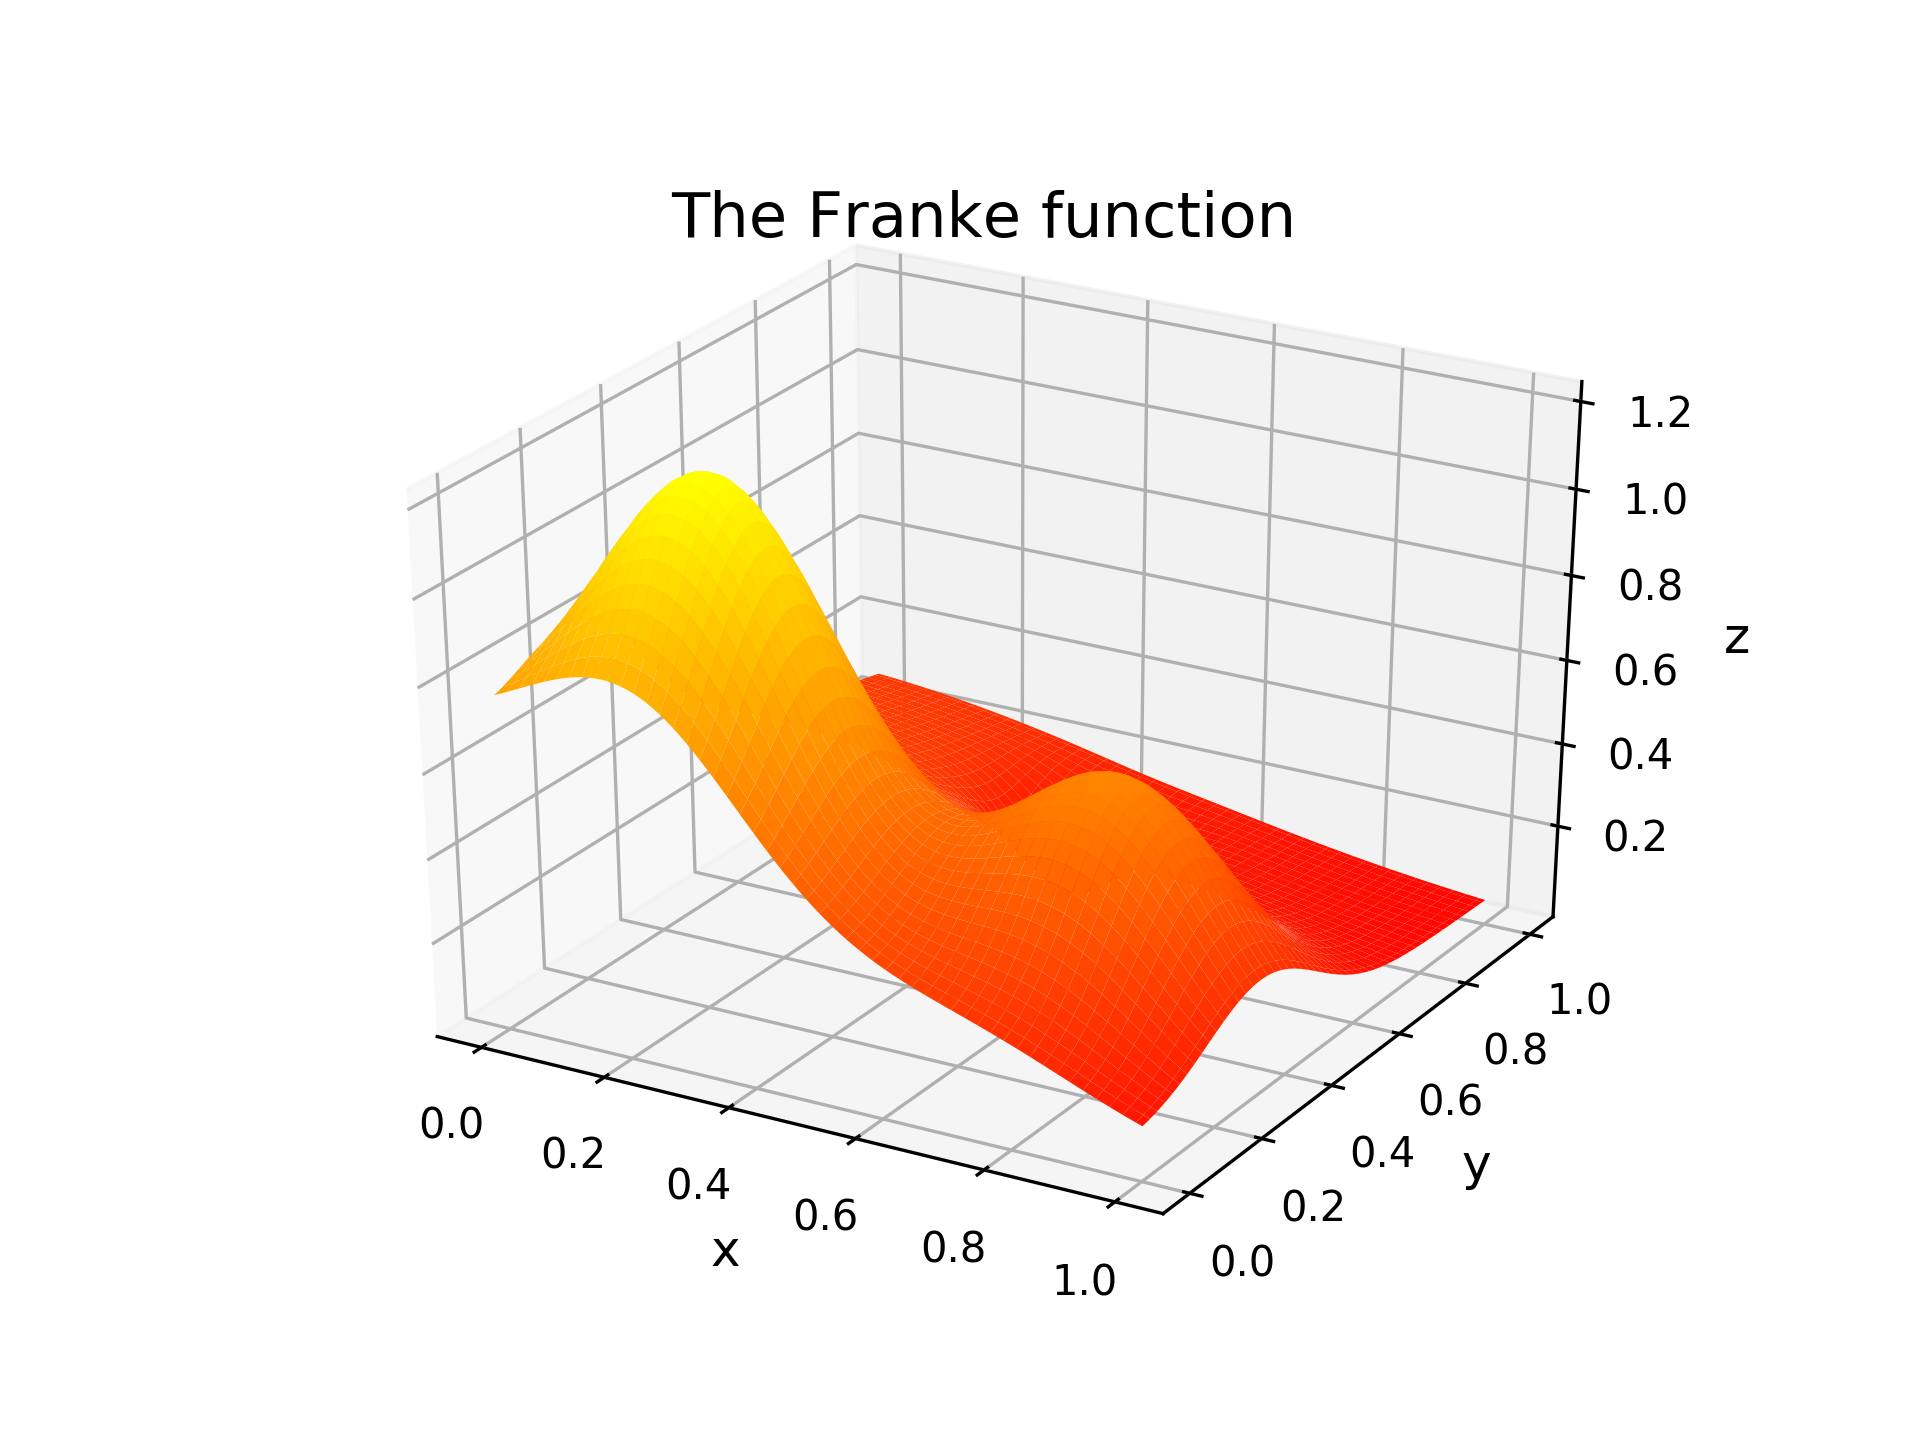
\includegraphics[width=0.5\textwidth]{../Figures/franke_function.png}
	\caption{The Franke function}
	\label{frankefunc}
\end{figure}
In order to get a better feel for how our methods work and the quality of our models, we will begin by studying a known function with added noise. The function we will be using is known as the Franke function: 
\begin{align}
	f(x,y)=&\frac{3}{4}\exp\Big(-\frac{(9x-2)^2}{4}-\frac{(9y-2)^2}{4}\Big)\nonumber\\
	&+\frac{3}{4}\exp\Big(-\frac{(9x+1)^2}{49}-\frac{(9y+1}{10}\Big)\nonumber\\
	&+\frac{1}{2}\exp\Big(-\frac{(9x-7)^2}{4}-\frac{(9y-3)^2}{4}\Big)\nonumber\\
	&-\frac{1}{5}\exp\Big(-(9x-4)^2-(9y-7)^2\Big)
\end{align} 
The function is defined for $x,y\in [0,1]$. Figure \ref{frankefunc} shows a 3D plot of the Franke function. \\[2mm]
For our purposes we need to add some noise to the Franke function. We add a noise which is normally distributed with mean 0 and standard deviation 1.\\[2mm]
We will first study the OLS model. We begin by investigating the naive approach by finding the MSE as a function of model complexity. Then we move on to a more in-depth analysis with the bias-variance tradeoff and 5fold cross validation. We then use the results from these processes to select and optimal degree for approximation. Finally, we compute the squared difference between this prediction and the true Franke function.\\[2mm]
As previously mentioned, the plain training/testing MSE does not give an accurate estimate of the actual error. We will therefore skip this step for the other methods. \\[2mm]
For the ridge regression method we begin by studying the bias variance tradeoff and the 5fold cross validation in order to determine the best value of the penalty $\lambda$. We then make an approximation using this value. The errors are studied in the same way as for OLS. \\[2mm]
When it comes to lasso regression, the procedure will be the same as for ridge regression.
\newpage
\subsubsection{Predicting terrain data}
The next step is to use our models to predict terrain data. The original terrain data\footnote{The data were downloaded from the \href{https://github.com/CompPhysics/MachineLearning/tree/master/doc/Projects/2020/Project1/DataFiles}{MachineLearning GitHub}.} is plotted in figure \ref{terrain}. \\[2mm]
For this part of the project we will repeat the analysis done for the Franke function as described in the previous section. The only difference is that for ridge and lasso we will perform a grid search in order to obtain a first rough estimate of the best polynomial degree and $\lambda$-combination. This will be done by computing (naively) the MSE for a set of combinations. This process will be used to determine a polynomial degree for which we will then use 5fold cross validation and the bias variance tradeoff for determining the best penalty $\lambda$.


\section{Results}
Figure \ref{fig3} shows how the MSE varies as a function of the model complexity (polynomial degree) for the OLS approximation of the Franke function. Figure \ref{fig4} shows the bias variance tradeoff for the OLS approximation of the Franke function using bootstrap resampling. Figure \ref{fig5} shows the corresponding 5fold cross validation results. Based on the latter plot, an OLS approximation using a 4th order polynomial was made. This is presented in figure \ref{fig1}. The squared difference between the approximation and the true Franke function is shown in figure \ref{fig2}. \\[2mm]
Figure \ref{fig6} shows the bias variance tradeoff of the 5th degree ridge approximation of the Franke function for a variety of penalties $\lambda$. Figure \ref{fig7} shows the corresponding 5fold cross validation. Based on the latter, $\lambda=10^{-2}$ was chosen. The resulting approximation and error is shown in figures \ref{fig8} and \ref{fig9} respectively. \\[2mm]
Figure \ref{fig10} shows the bias variance tradeoff of the 5th degree lasso approximation for a variety of penalties $\lambda$. Figure \ref{fig11} shows the corresponding 5fold cross validation. Based on the latter, $\lambda=10^{-4}$ was chosen. The resulting approximation and error is shown in figures \ref{fig12} and \ref{fig13} respectively. \\[2mm]
Figure \ref{fig14} shows the bias variance tradeoff of the terrain data OLS approximation.The corresponding 5fold cross validation is shown in figure \ref{fig15}. Figure \ref{fig16} shows the OLS approximation using a 5th order polynomial. The squared difference between the prediction and the original terrain data is shown in figure \ref{fig17}.\\[2mm]
Figure \ref{fig18} shows the test MSE for each combination of penalties $\lambda$ and polynomial degrees for ridge regression of the terrain data. Figure \ref{fig19} shows the bias variance tradeoff for the 4th degree polynomial approximation. Figure \ref{fig20} shows the corresponding 5fold cross validation. Figure \ref{fig21} shows the ridge approximation of the terrain data with a 4th degree polynomial and penalty $\lambda=10$. The corresponding errors are shown in figure \ref{fig22}.\\[2mm]
Figure \ref{fig23} shows the test MSE for each combination of penalties $\lambda$ and polynomial degrees for lasso regression of the terrain data. Figure \ref{fig24} shows the bias variance tradeoff for the 3rd degree polynomial approximation. Figure \ref{fig25} shows the corresponding 5fold cross validation. Figure \ref{fig26} shows the lasso approximation of the terrain data with a 3rd degree polynomial and penalty $\lambda=10^{-4}$. The corresponding errors are shown in figure \ref{fig27}.

\onecolumngrid
~
\begin{figure}[h!]
 	\centering
  	\subfloat[2D plot of terrain data.]{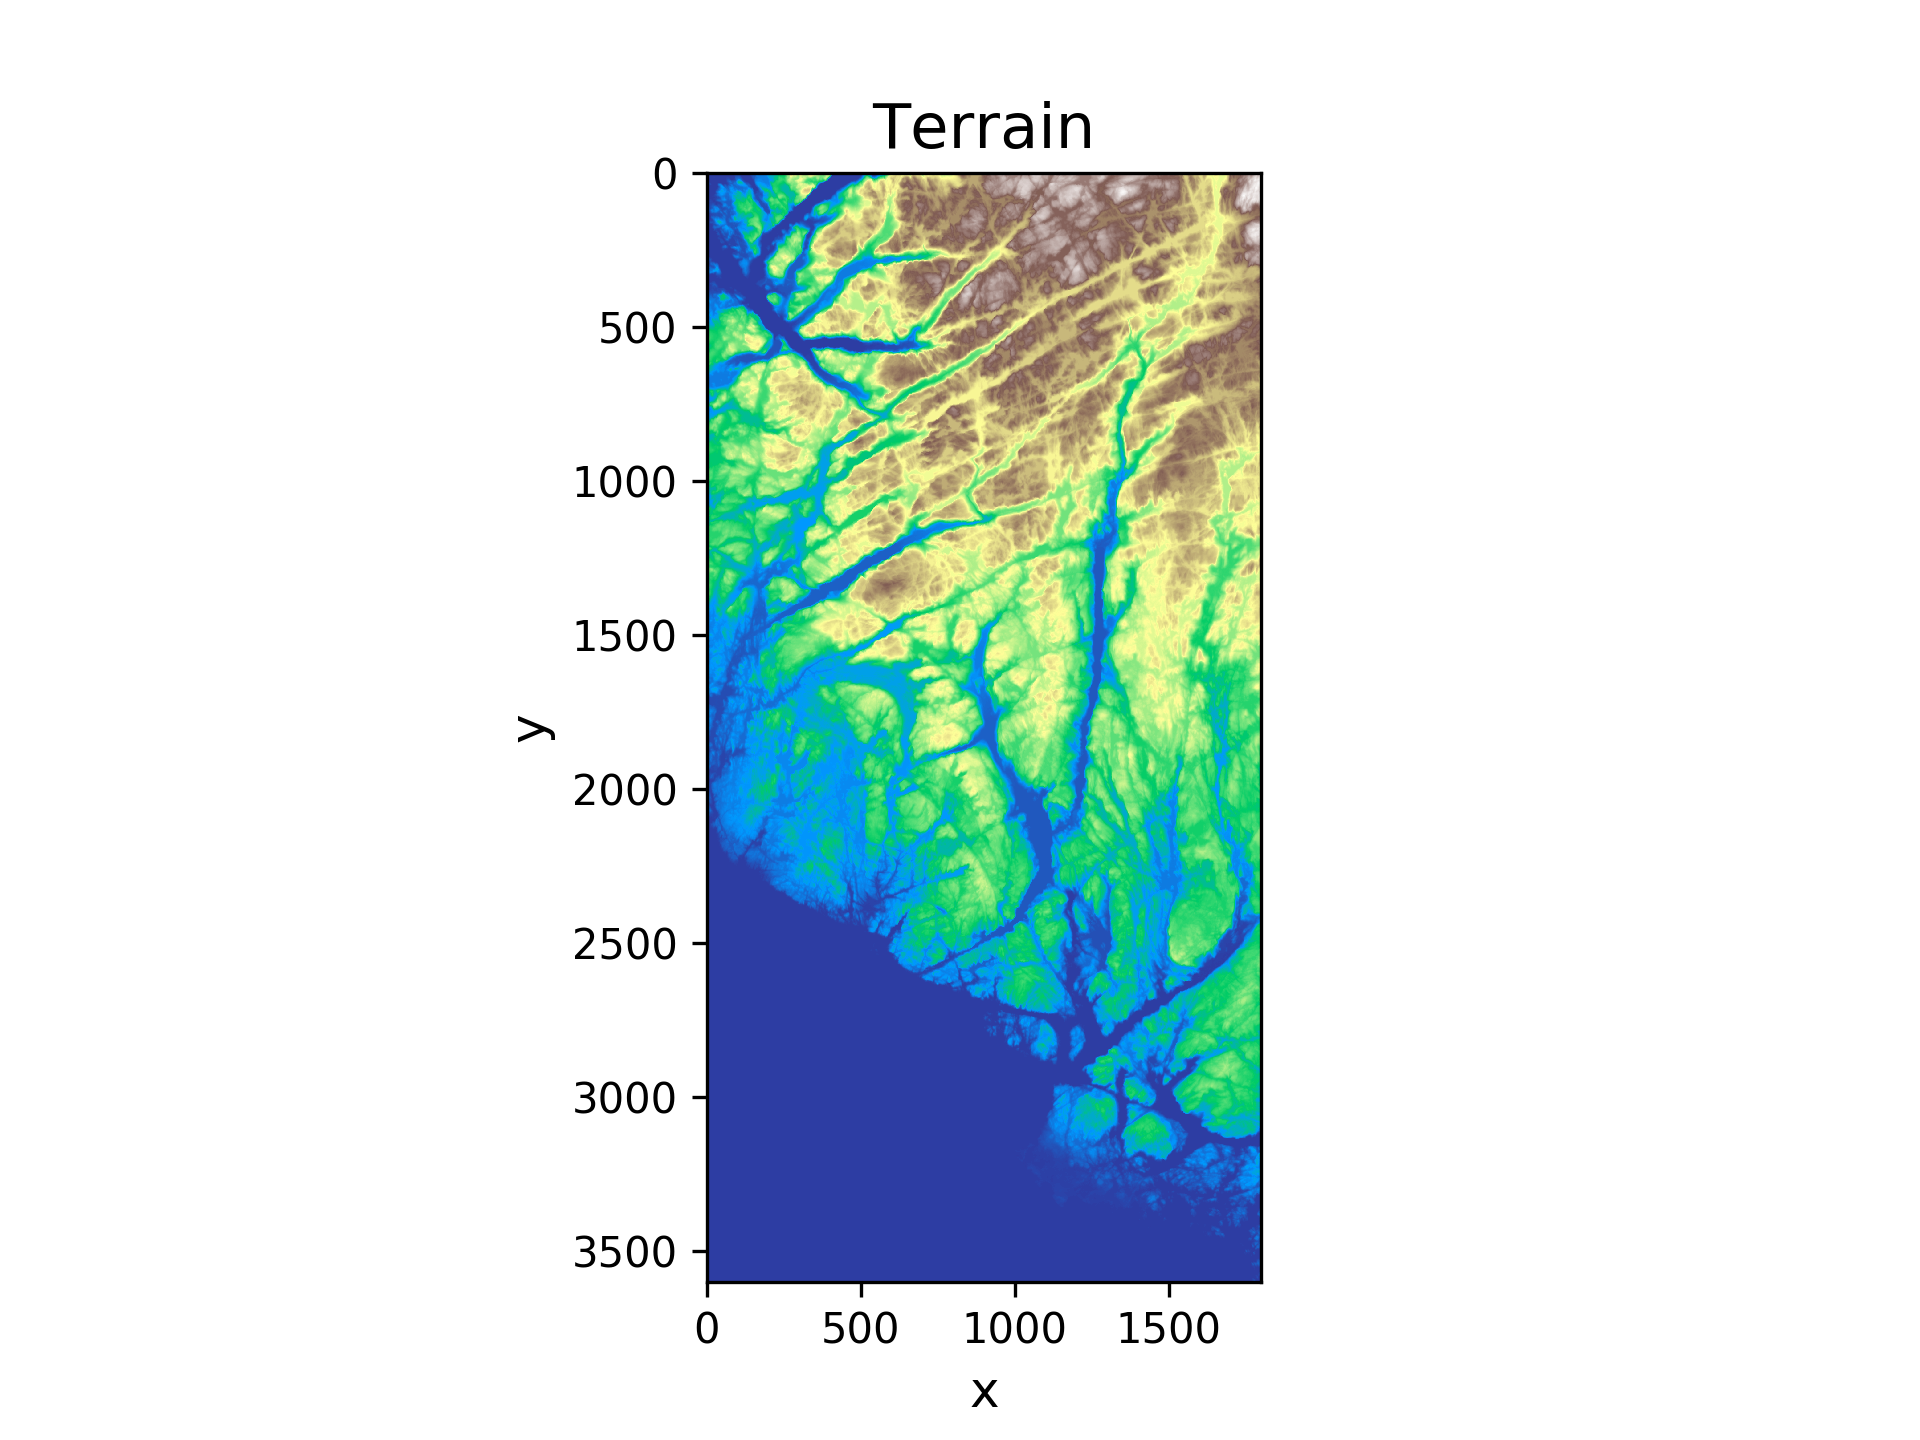
\includegraphics[width=0.5\textwidth]{../Figures/terrain.png}\label{terrain1}}
  	\subfloat[3D plot of terrain data.]{\includegraphics[width=0.5\textwidth]{../Figures/terrain3D_adjusted.png}\label{terrain2}}
  	\caption{The terrain of Møsvatn Austfjell in Norway.}
	\label{terrain}
\end{figure}

\twocolumngrid

\begin{figure}
	\centering
	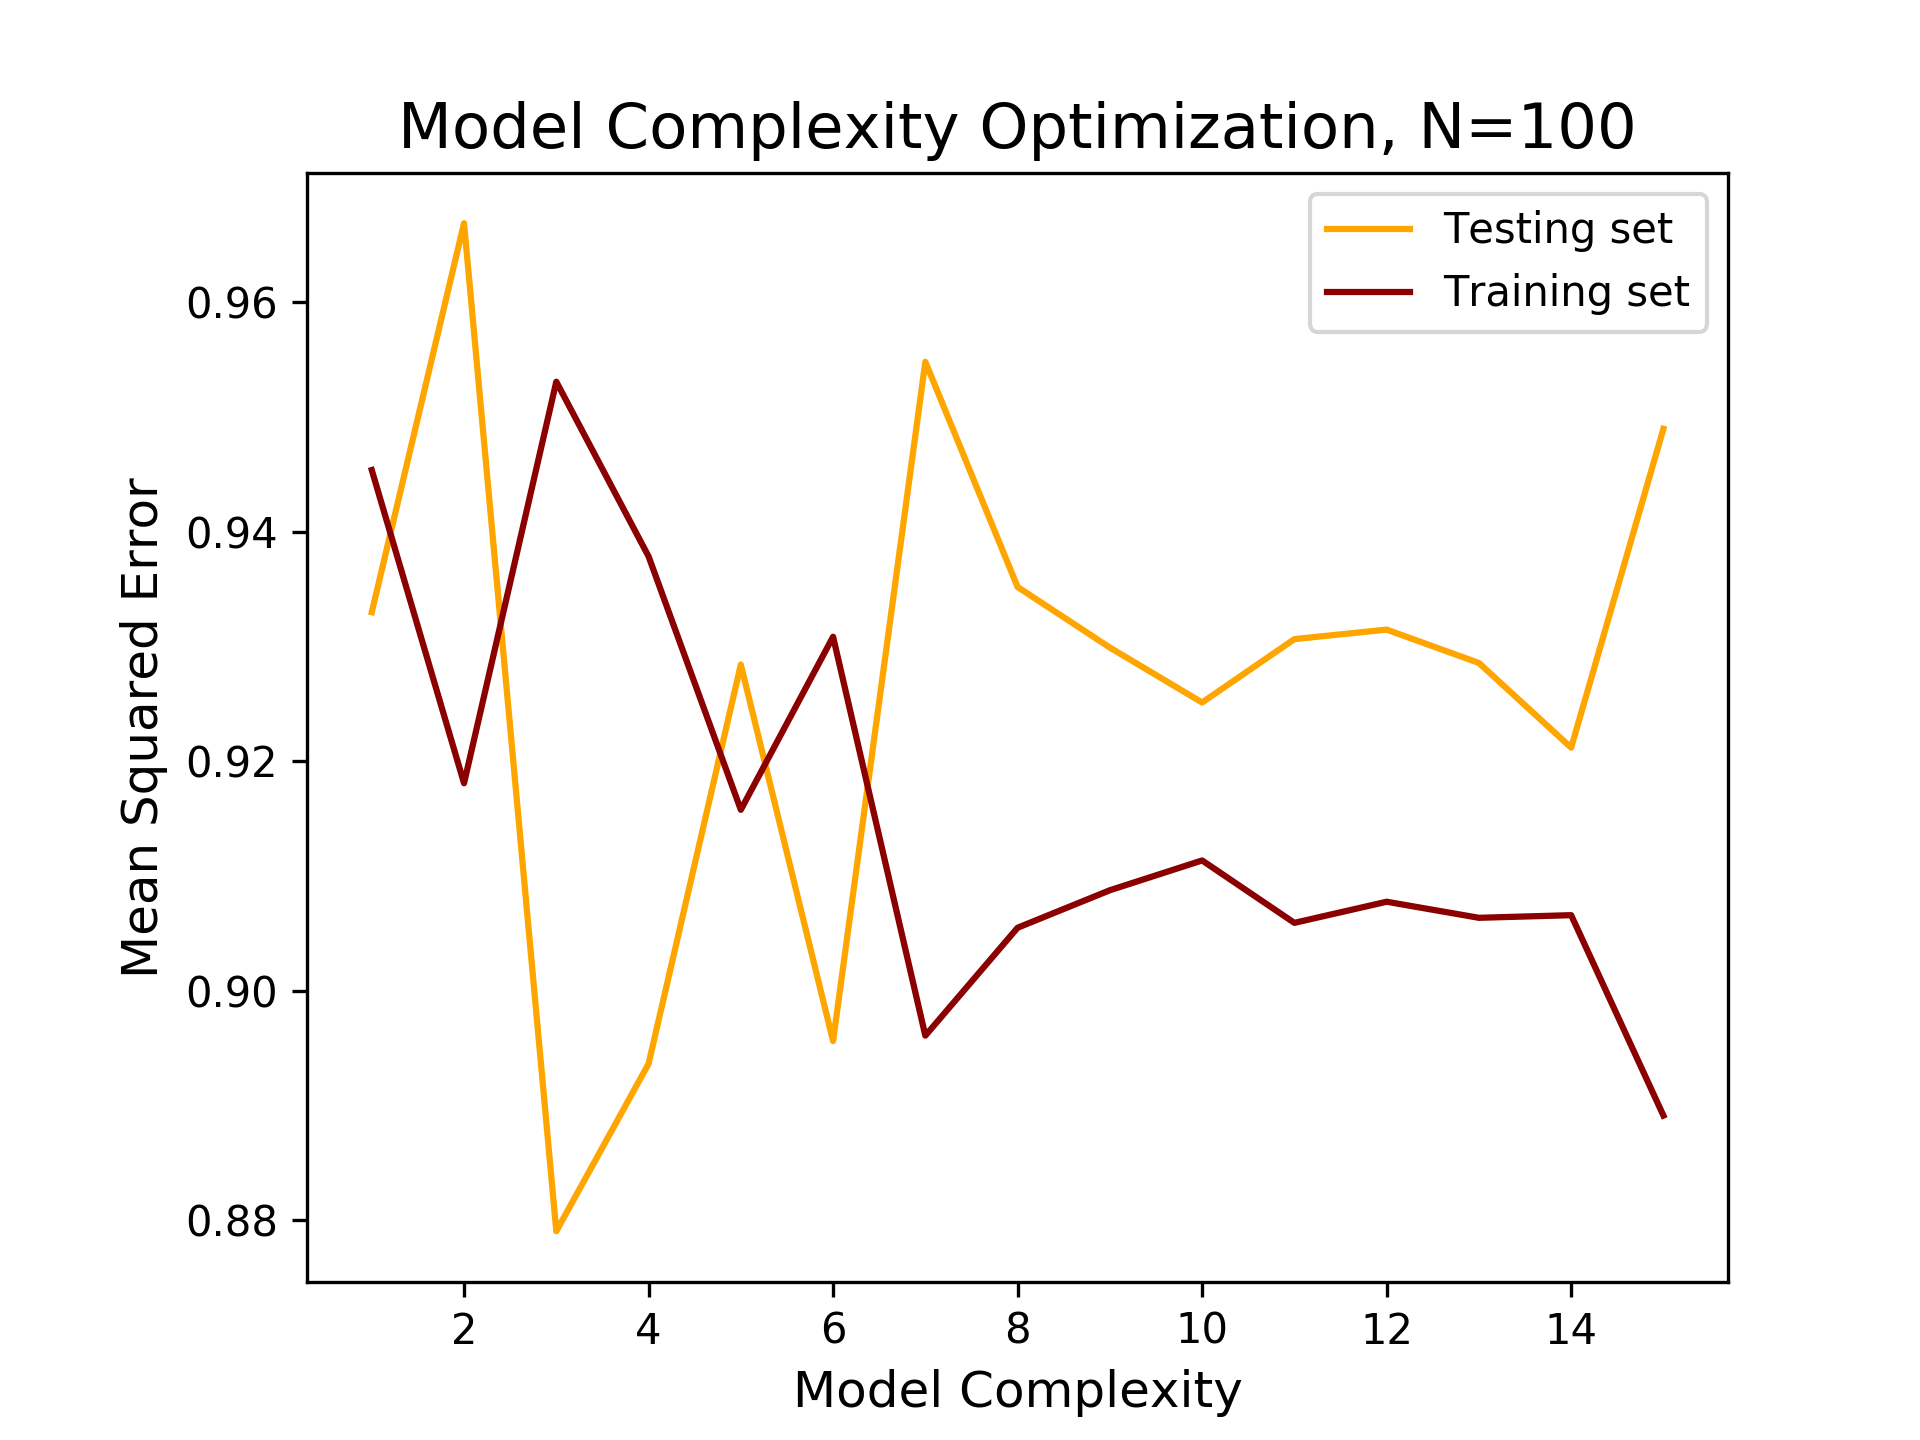
\includegraphics[width=0.45\textwidth]{../Figures/model_complexity_mse_franke_N100.png}
	\caption{MSE as a function of model complexity for the Franke function OLS approximation.}
	\label{fig3}
\end{figure}
\begin{figure}
	\centering
	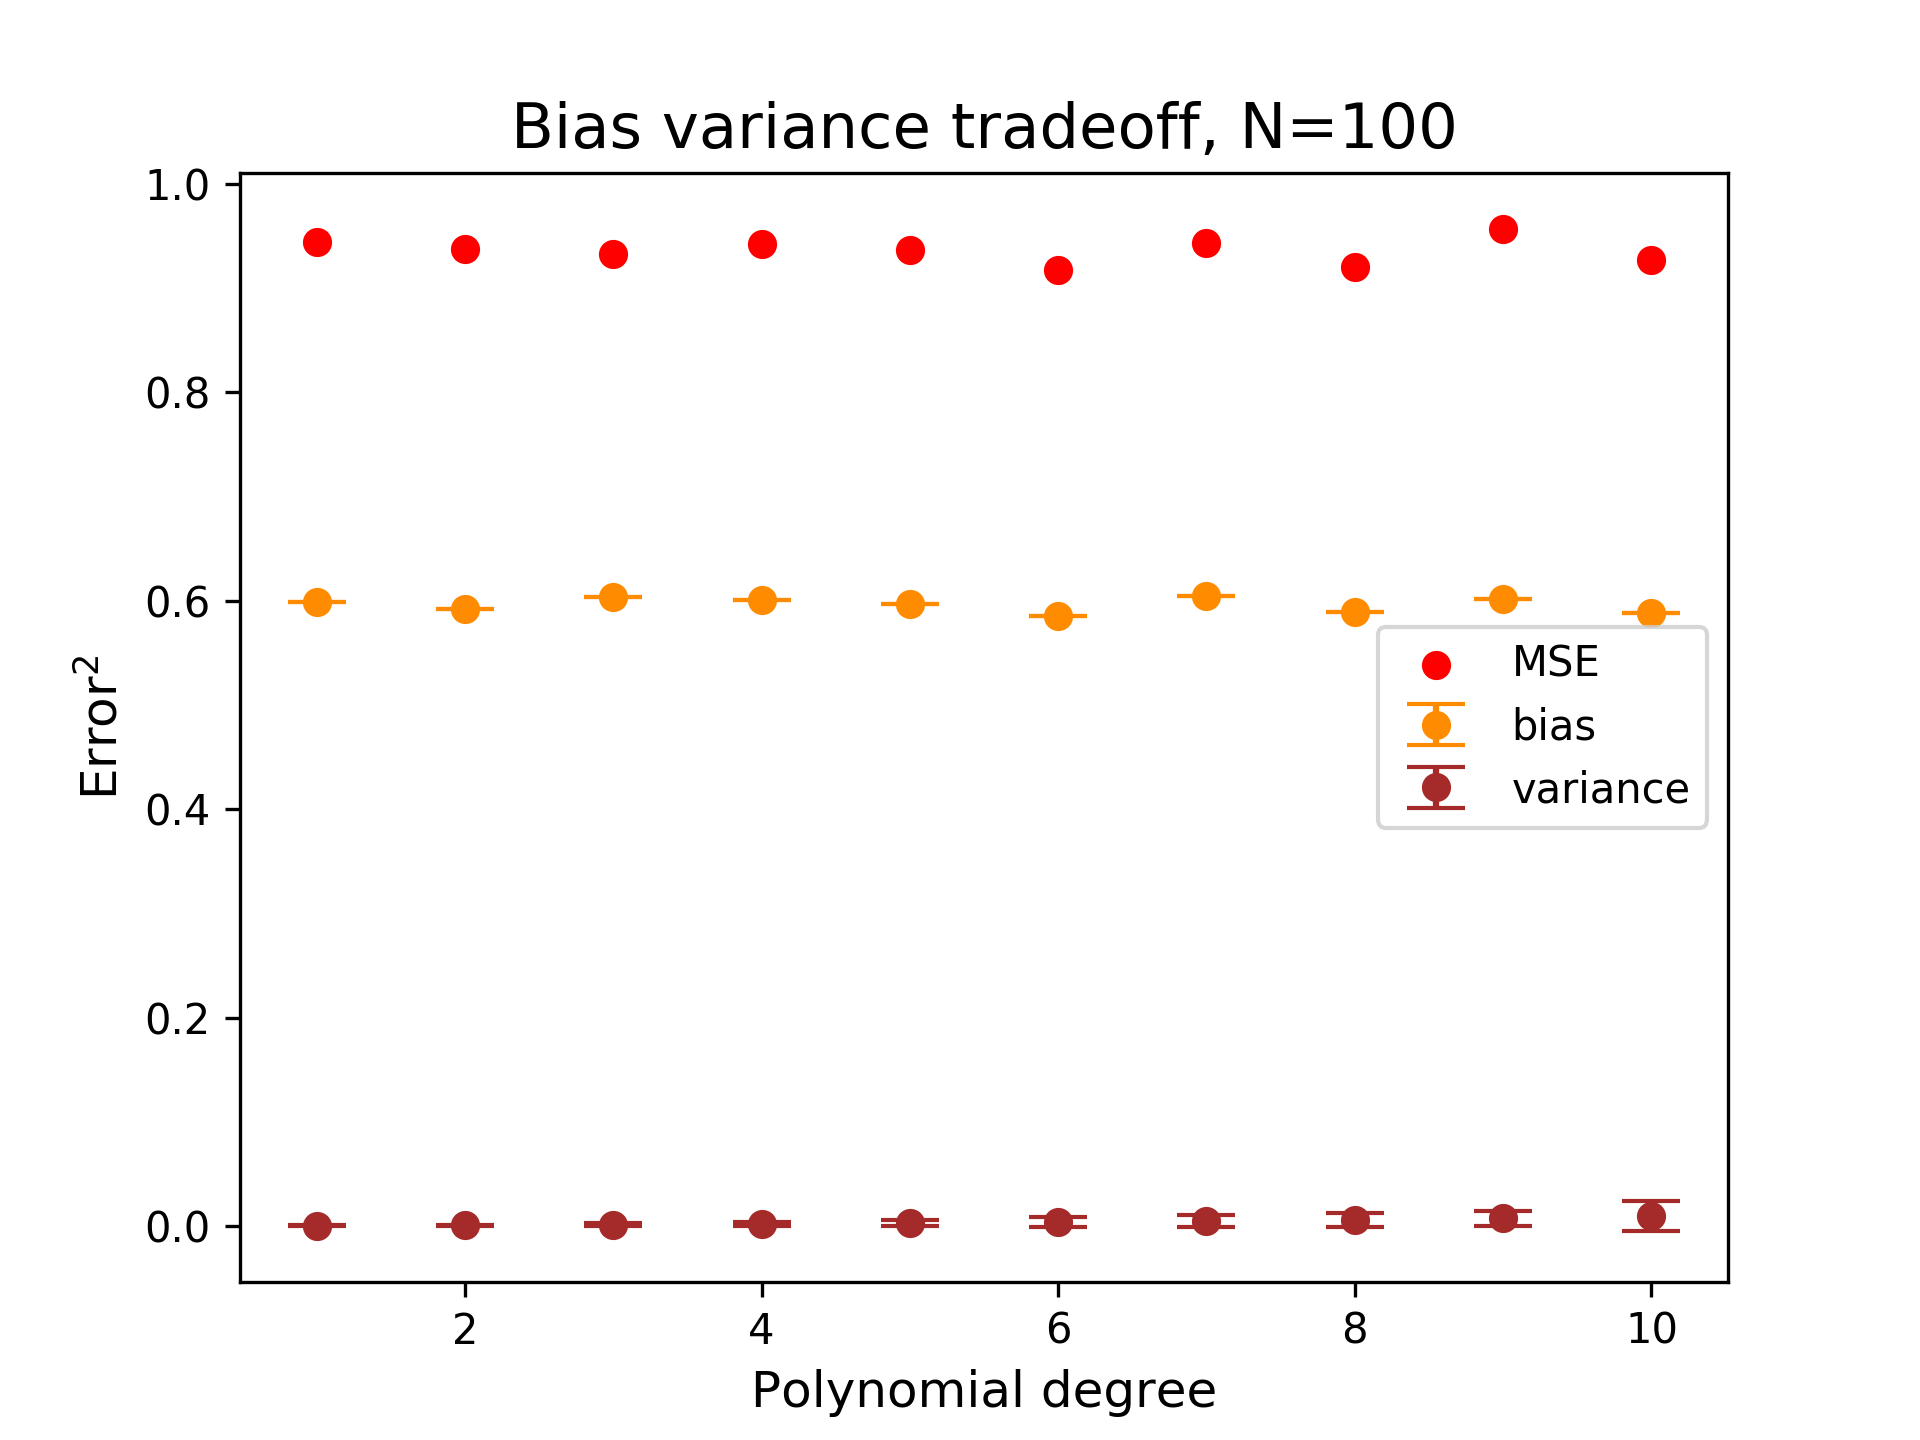
\includegraphics[width=0.45\textwidth]{../Figures/b-v_tradeoff_franke_N100.png}
	\caption{Bias variance tradeoff of the Franke function OLS approximation.}
	\label{fig4}
\end{figure}
\begin{figure}
	\centering
	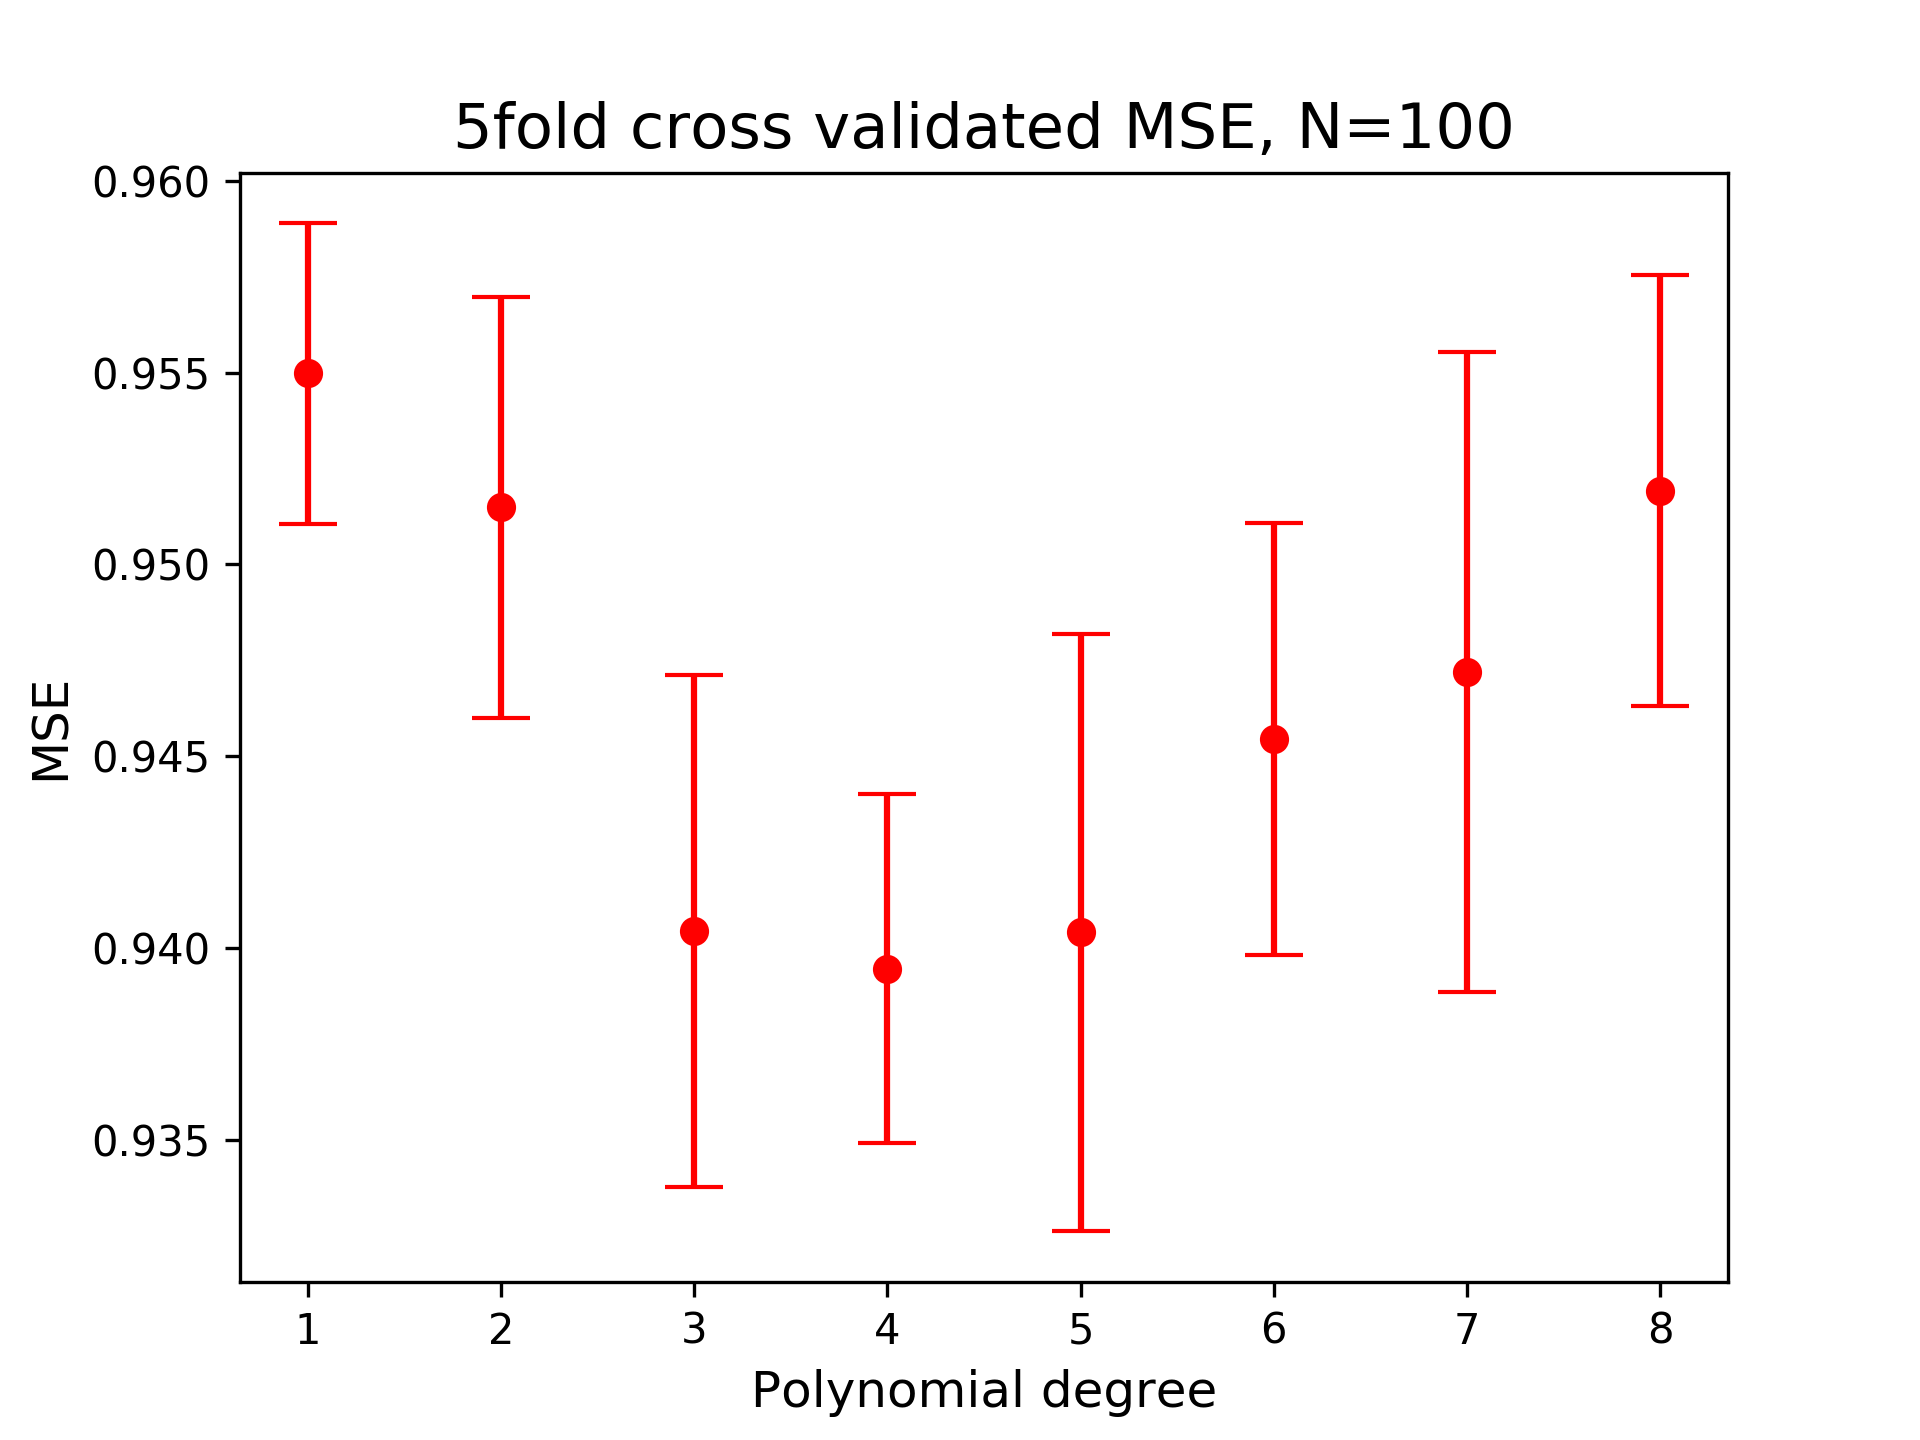
\includegraphics[width=0.45\textwidth]{../Figures/kfold_mse_N100.png}
	\caption{Cross validated MSE as a function of model complexity for the Franke function OLS approximation.}
	\label{fig5}
\end{figure}
\begin{figure}
 	\centering
	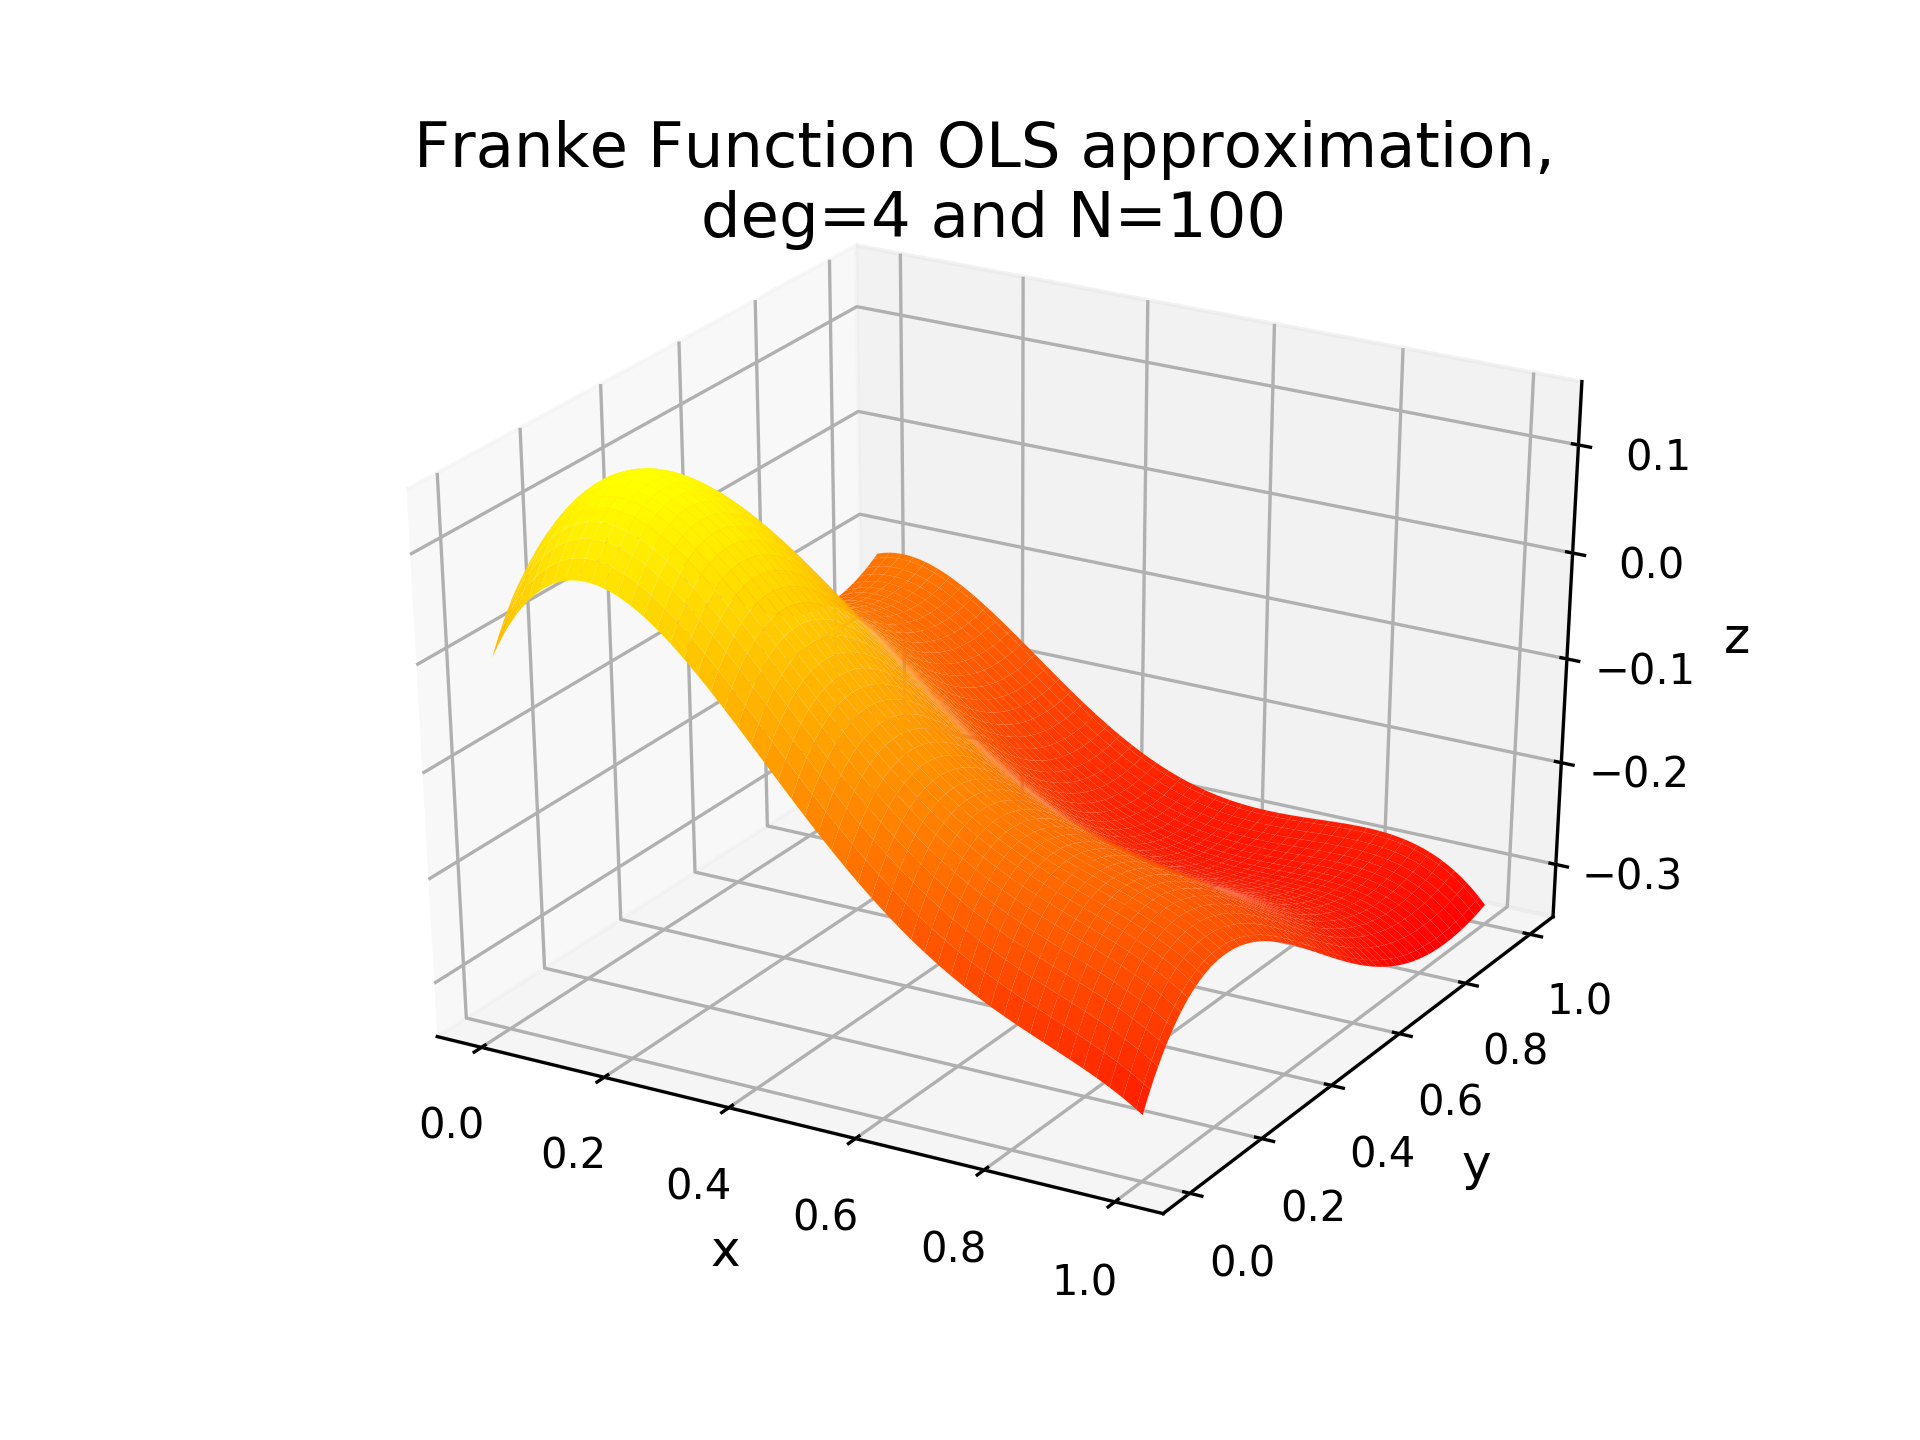
\includegraphics[width=0.45\textwidth]{../Figures/franke_OLS_deg4_N100.png}
  	\caption{OLS approximation of the Franke function by a 5th degree polynomial.}
	\label{fig1}
\end{figure}
\begin{figure}
 	\centering
  	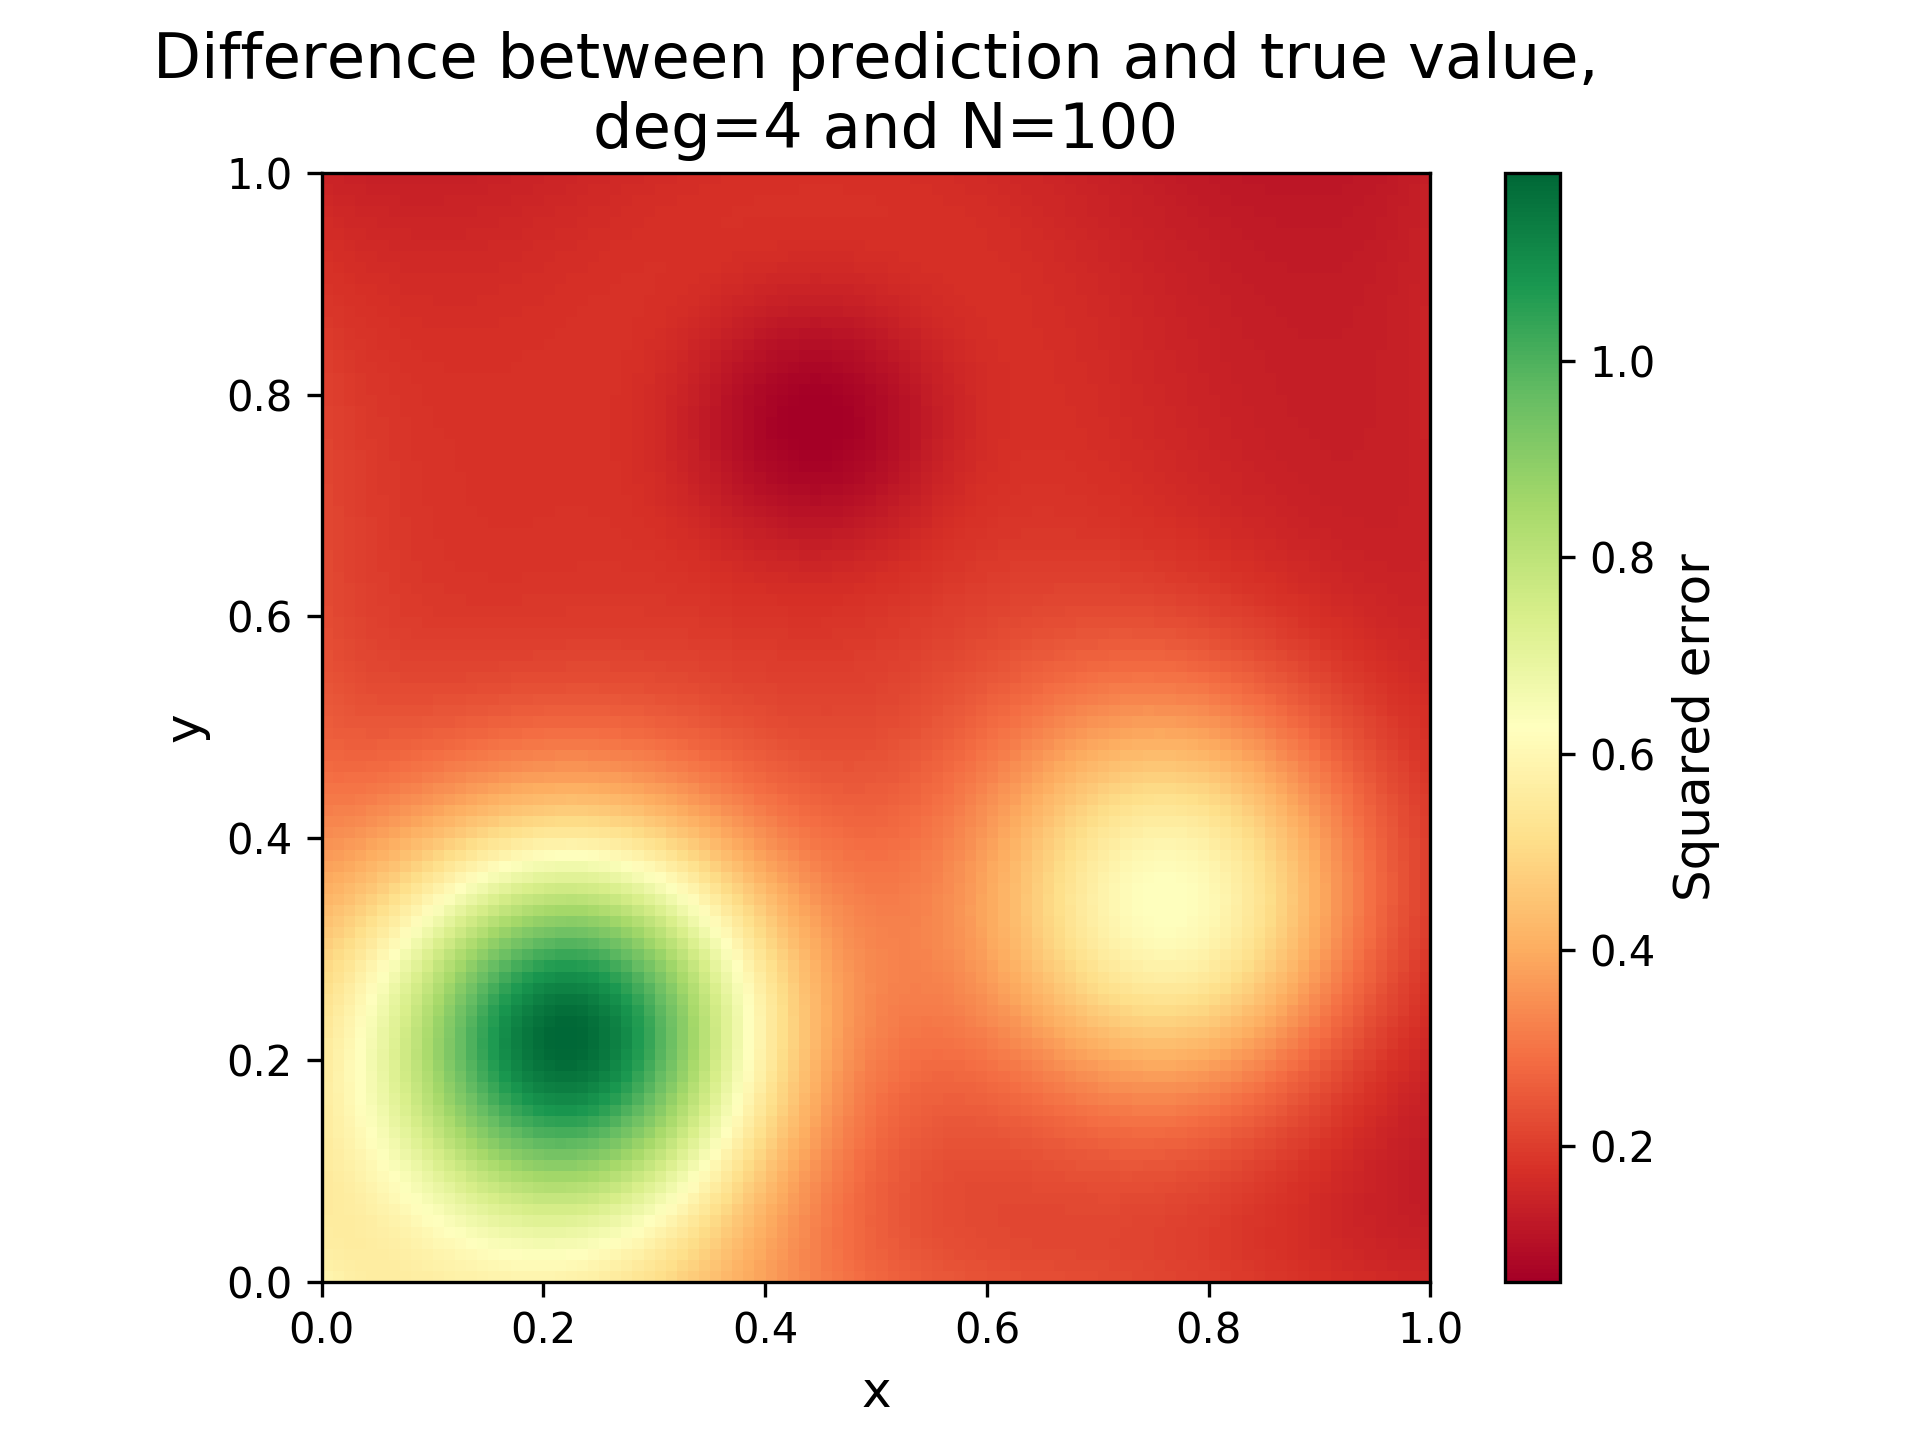
\includegraphics[width=0.45\textwidth]{../Figures/franke_OLS_error_deg4_N100.png}
  	\caption{The errors of the 5th degree OLS approximation of the Franke function.}
	\label{fig2}
\end{figure}

\begin{figure}
	\centering
	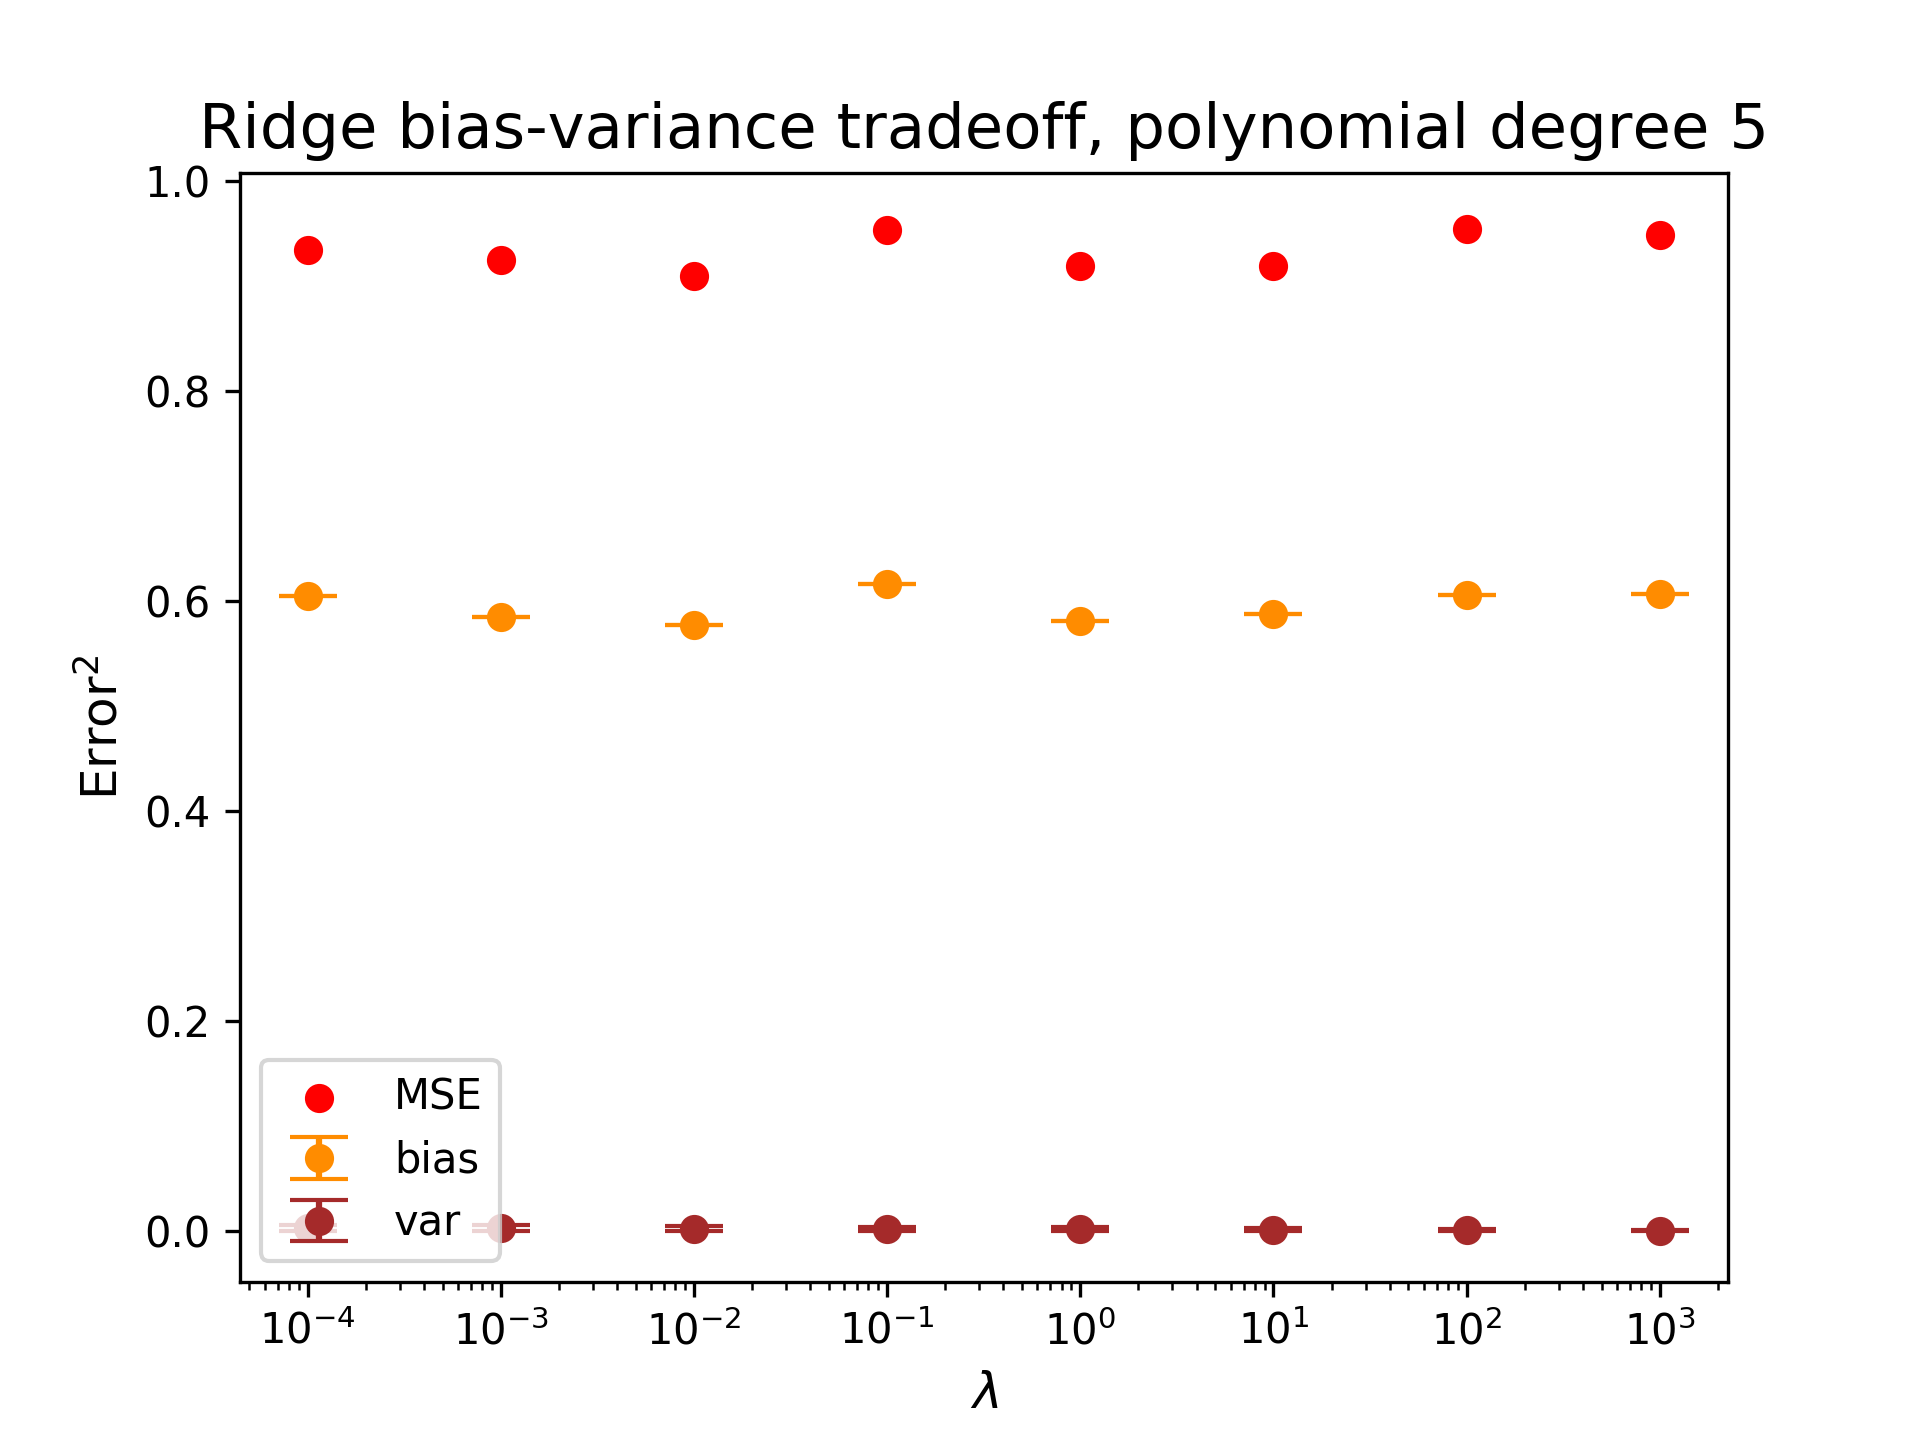
\includegraphics[width=0.45\textwidth]{../Figures/ridge_bias_variance_deg5.png}
	\caption{Bias variance tradeoff of the Franke function ridge approximation.}
	\label{fig6}
\end{figure}

\clearpage

\begin{figure}
	\centering
	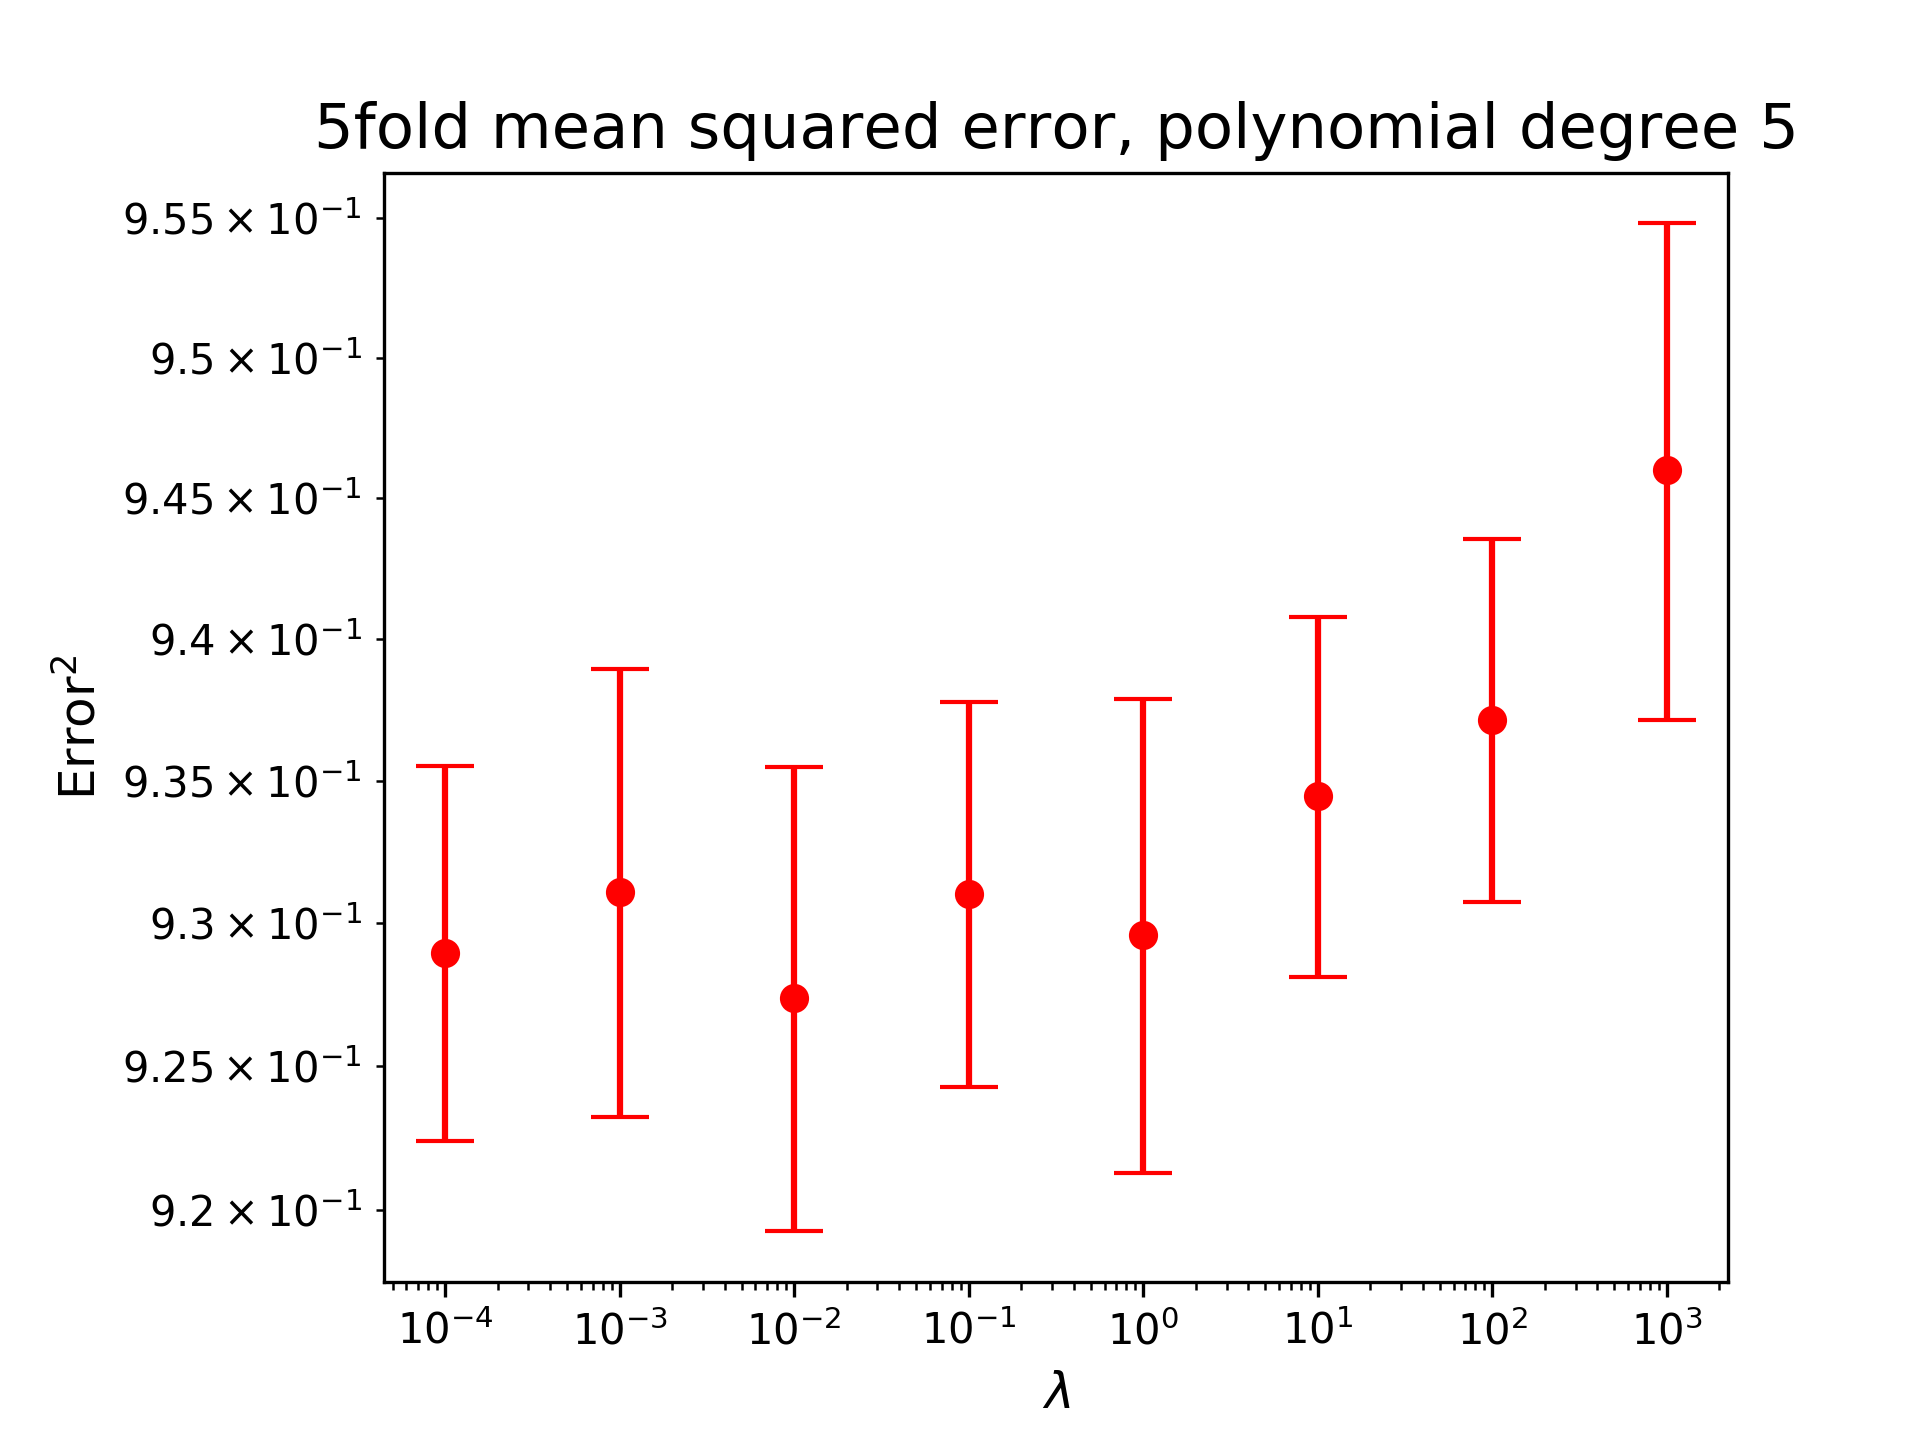
\includegraphics[width=0.45\textwidth]{../Figures/ridge_kfold_deg5.png}
	\caption{Cross validated MSE as a function of penalties $\lambda$ for the Franke function ridge approximation.}
	\label{fig7}
\end{figure}

\begin{figure}
 	\centering
	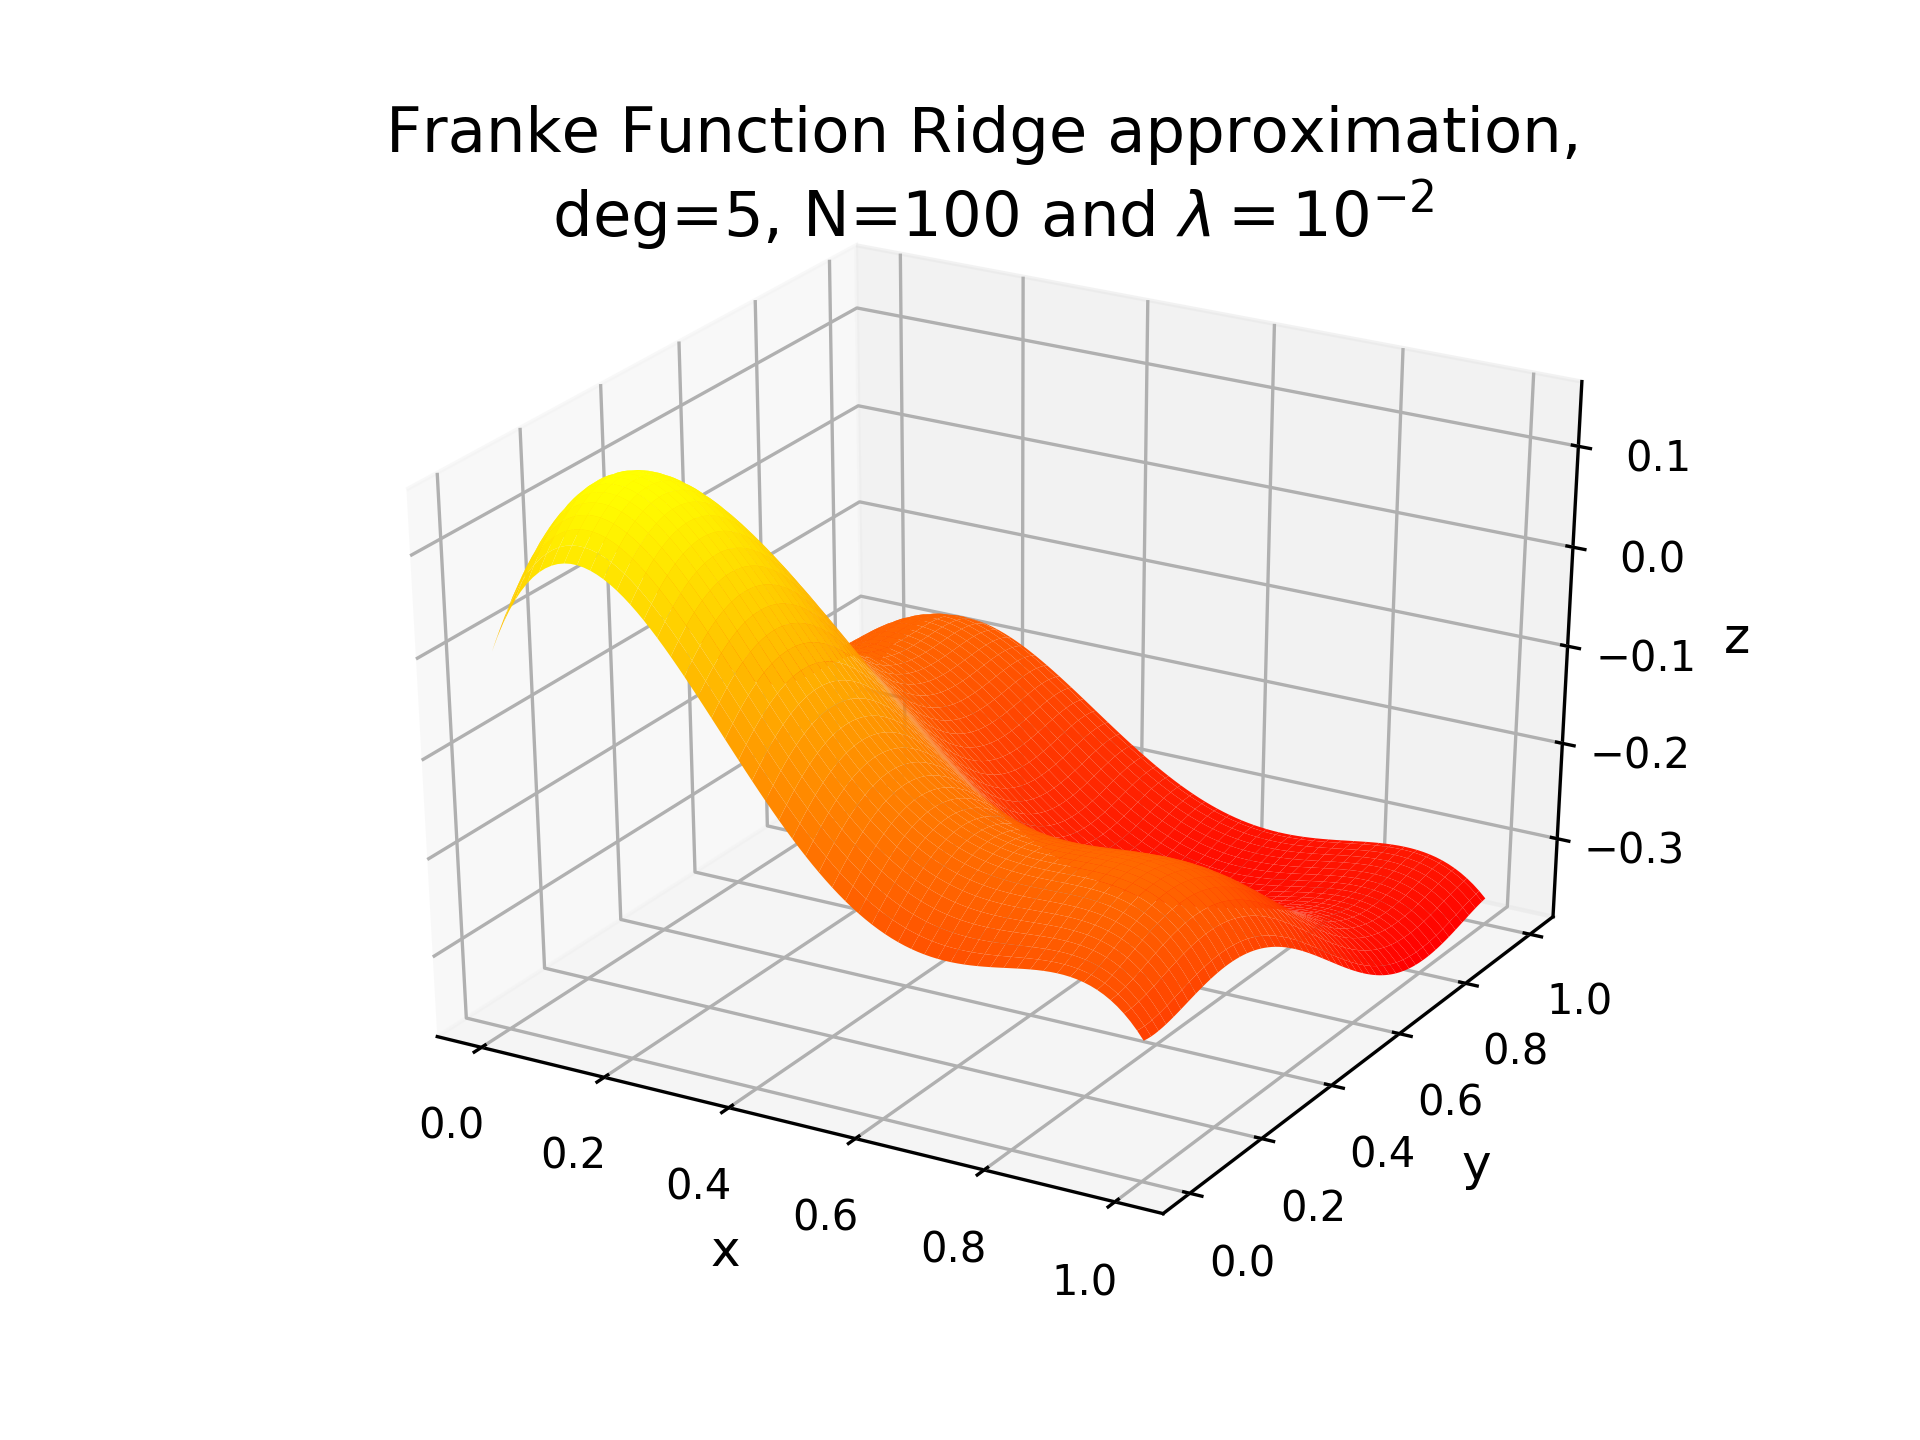
\includegraphics[width=0.45\textwidth]{../Figures/franke_ridge_deg5_N100.png}
  	\caption{Ridge approximation of the Franke function by a 5th degree polynomial using a penalty $\lambda=10^{-2}$.}
	\label{fig8}
\end{figure}

\begin{figure}
 	\centering
  	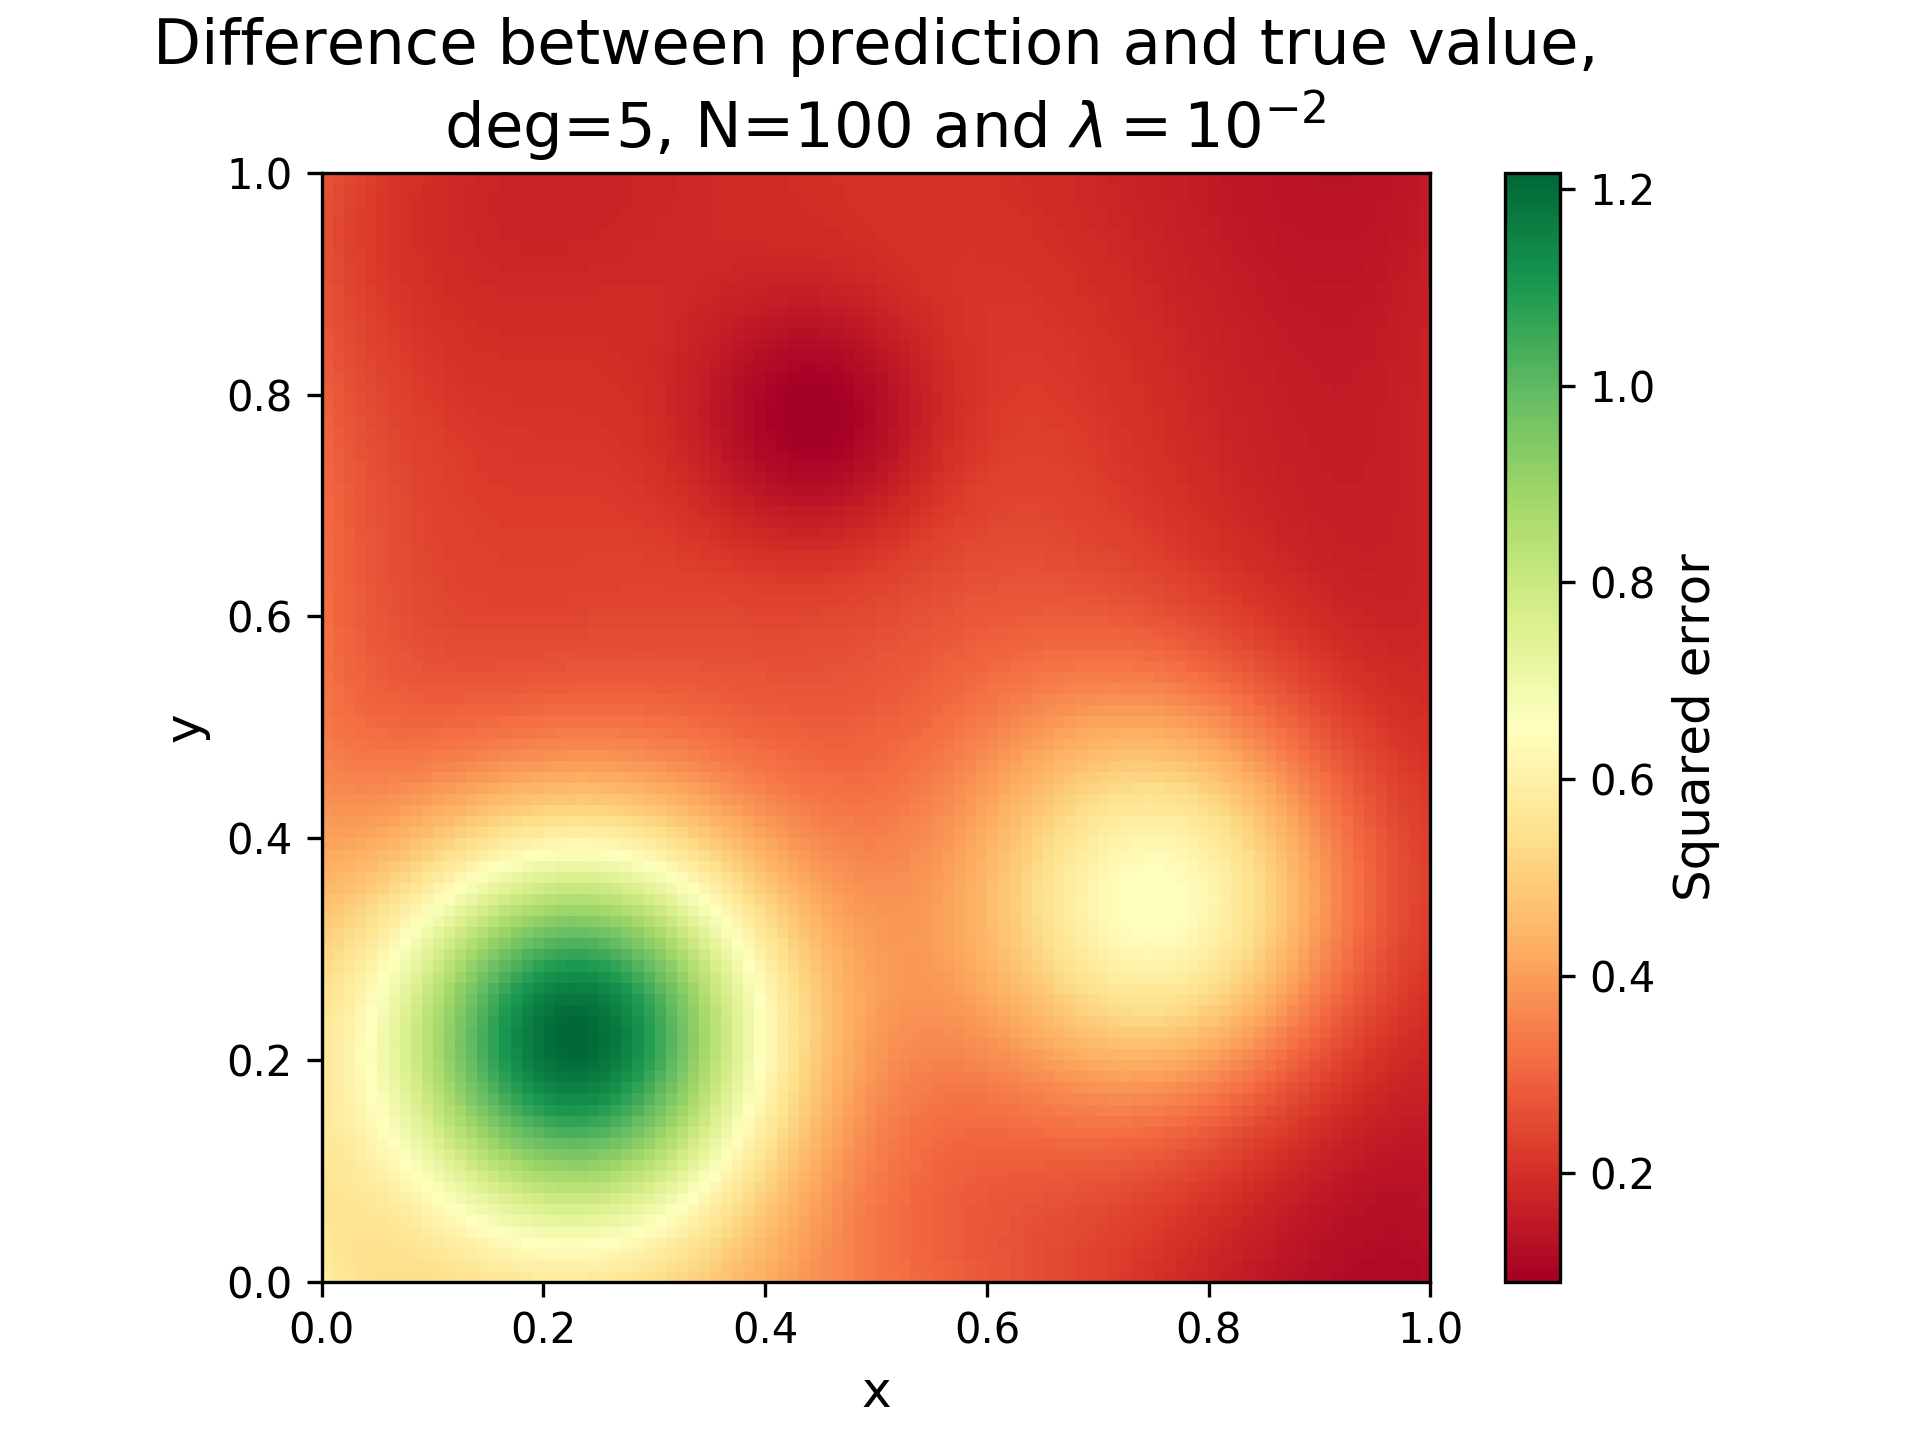
\includegraphics[width=0.45\textwidth]{../Figures/franke_ridge_error_deg5_N100.png}
  	\caption{The errors of the 5th degree ridge approximation of the Franke function with penalty $\lambda=10^{-2}$.}
	\label{fig9}
\end{figure}

\begin{figure}
	\centering
	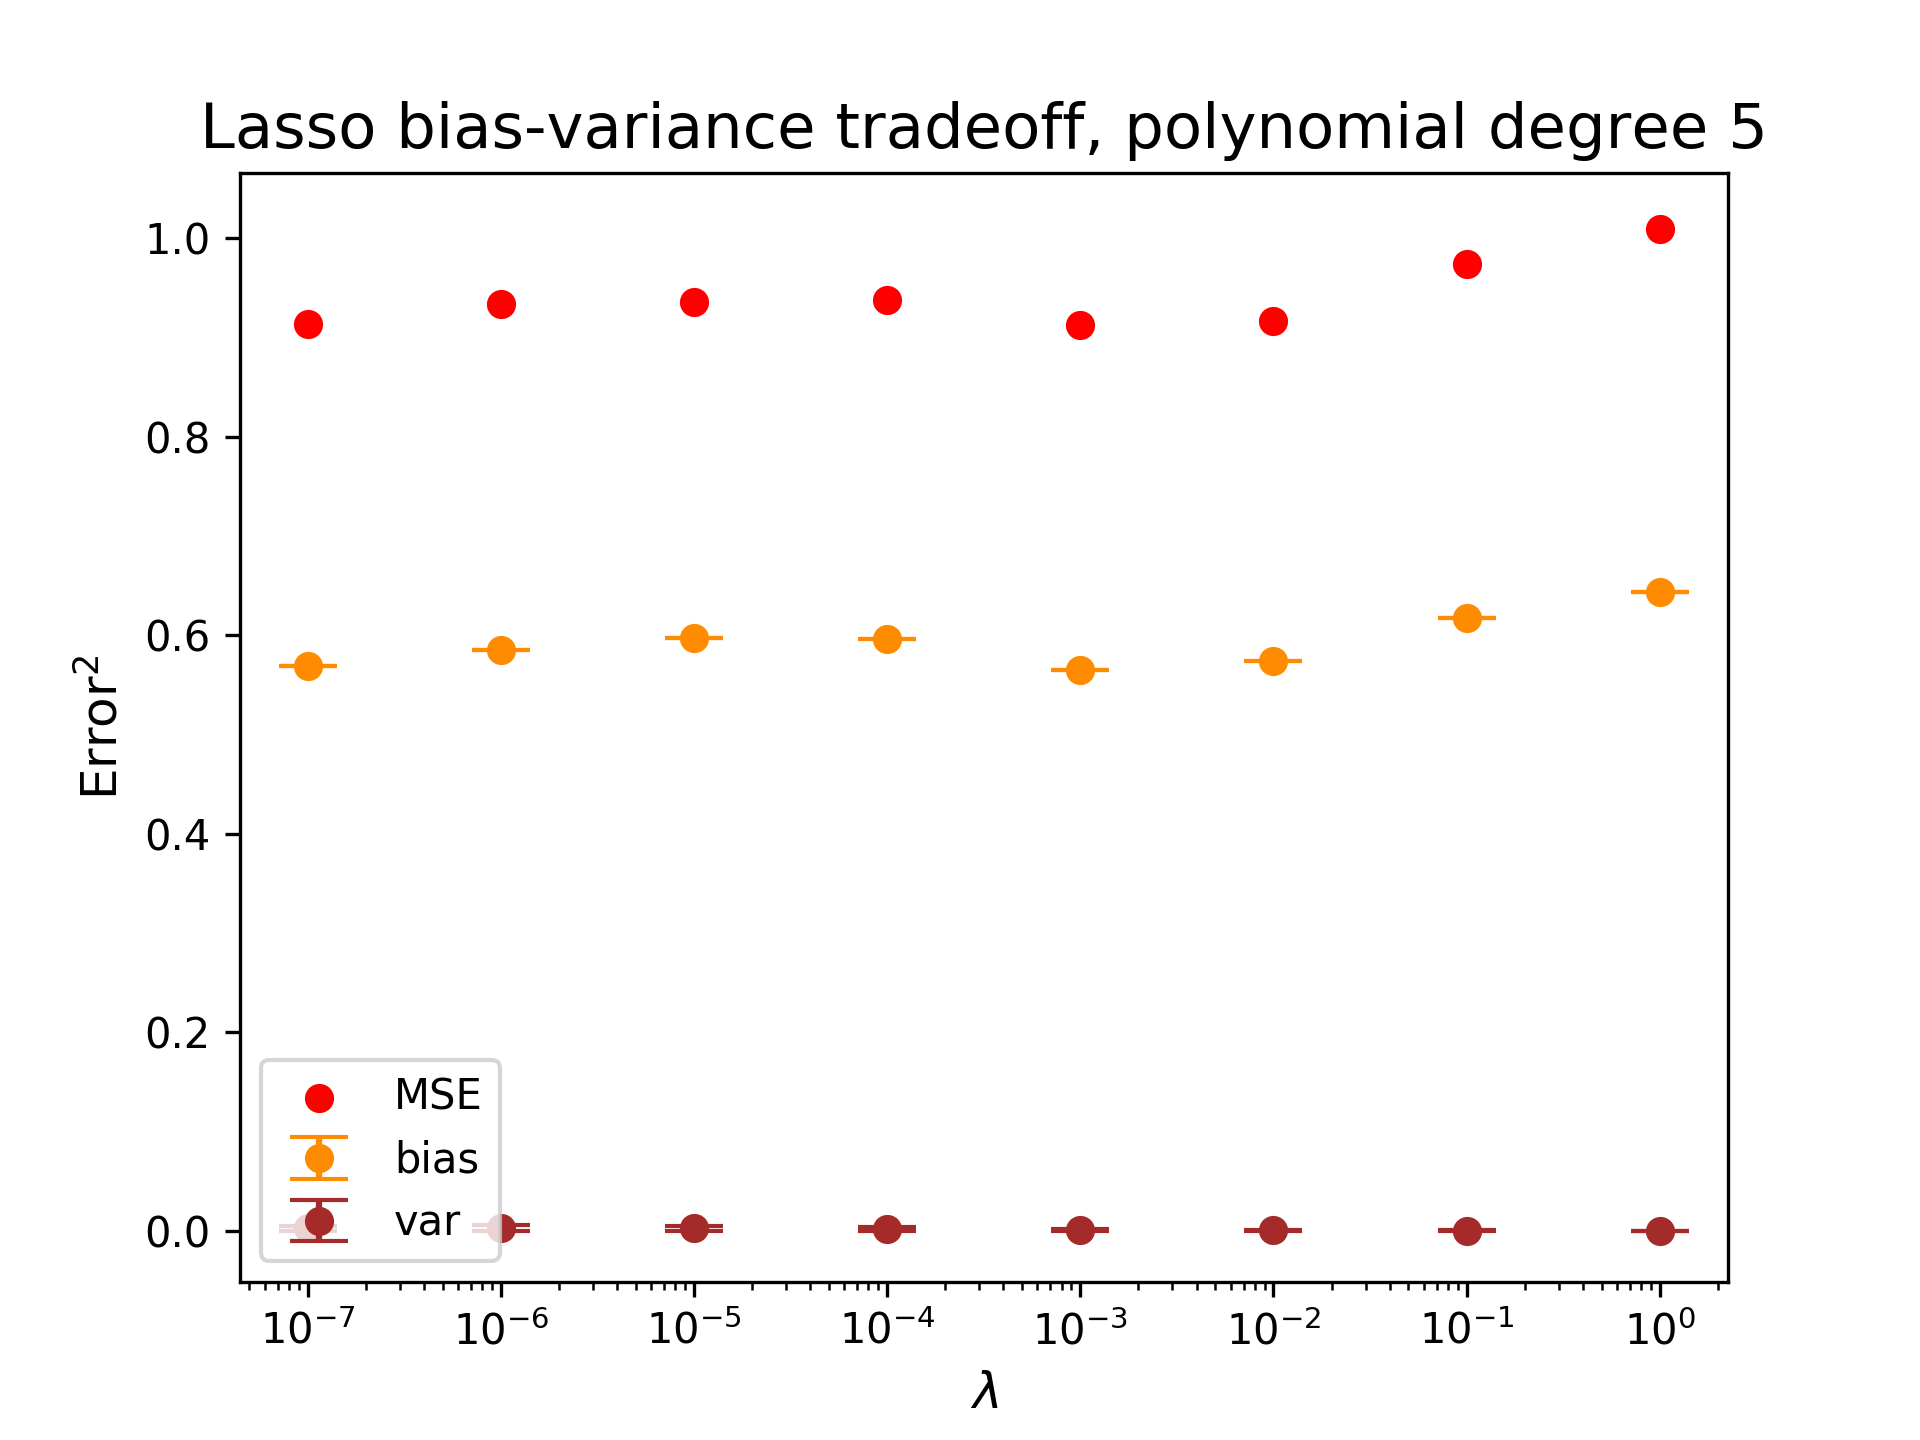
\includegraphics[width=0.45\textwidth]{../Figures/lasso_bias_variance_deg5.png}
	\caption{Bias variance tradeoff of the Franke function lasso approximation.}
	\label{fig10}
\end{figure}

\begin{figure}
	\centering
	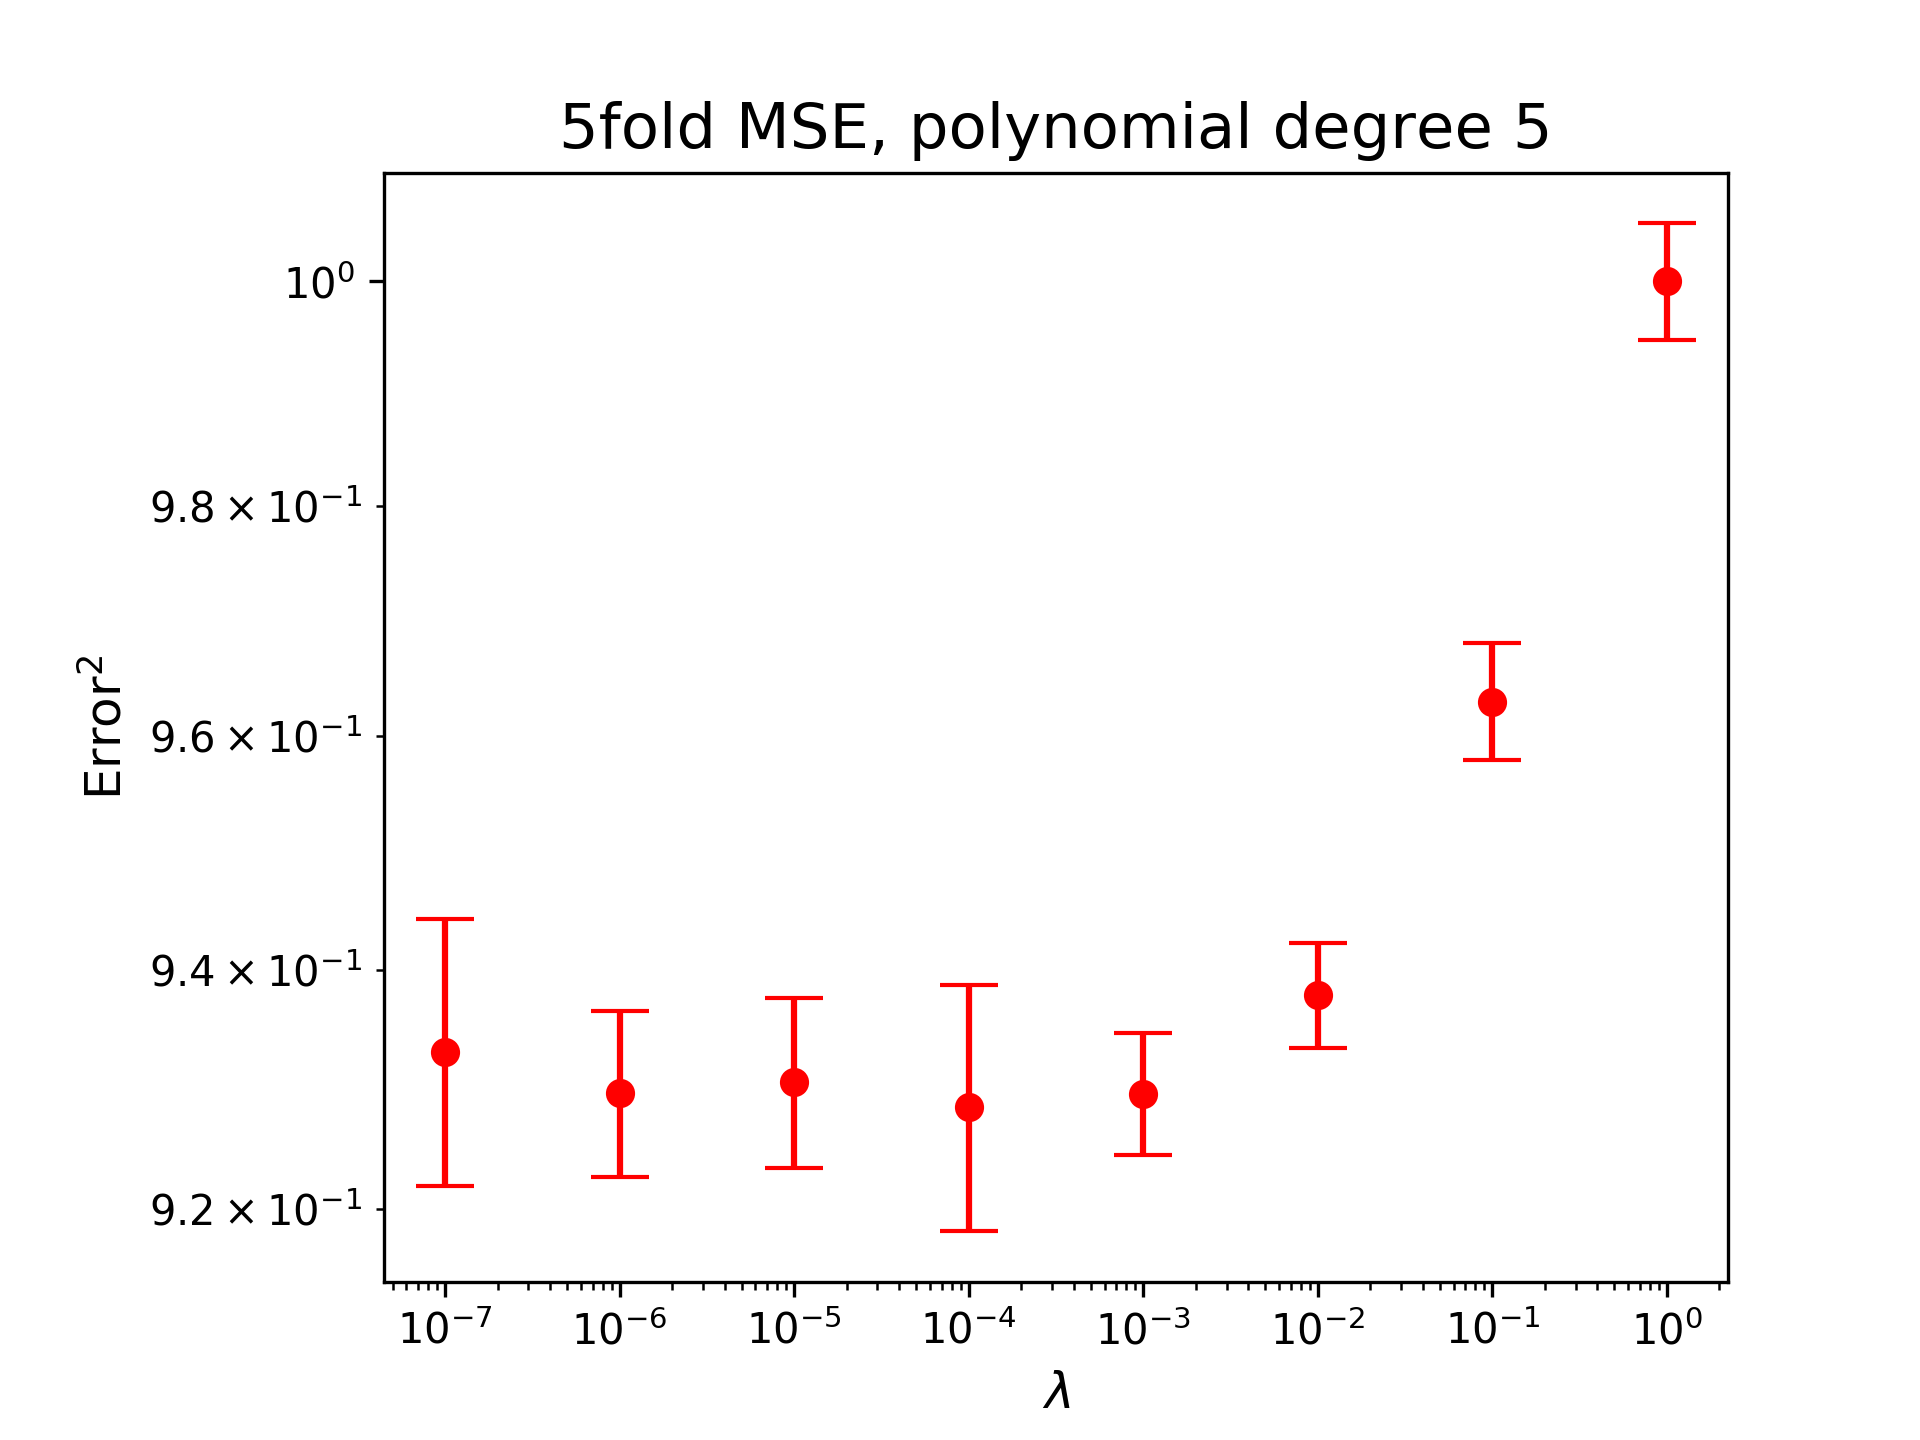
\includegraphics[width=0.45\textwidth]{../Figures/lasso_kfold_deg5.png}
	\caption{Cross validated MSE as a function of penalties $\lambda$ for the Franke function lasso approximation.}
	\label{fig11}
\end{figure}

\begin{figure}
 	\centering
	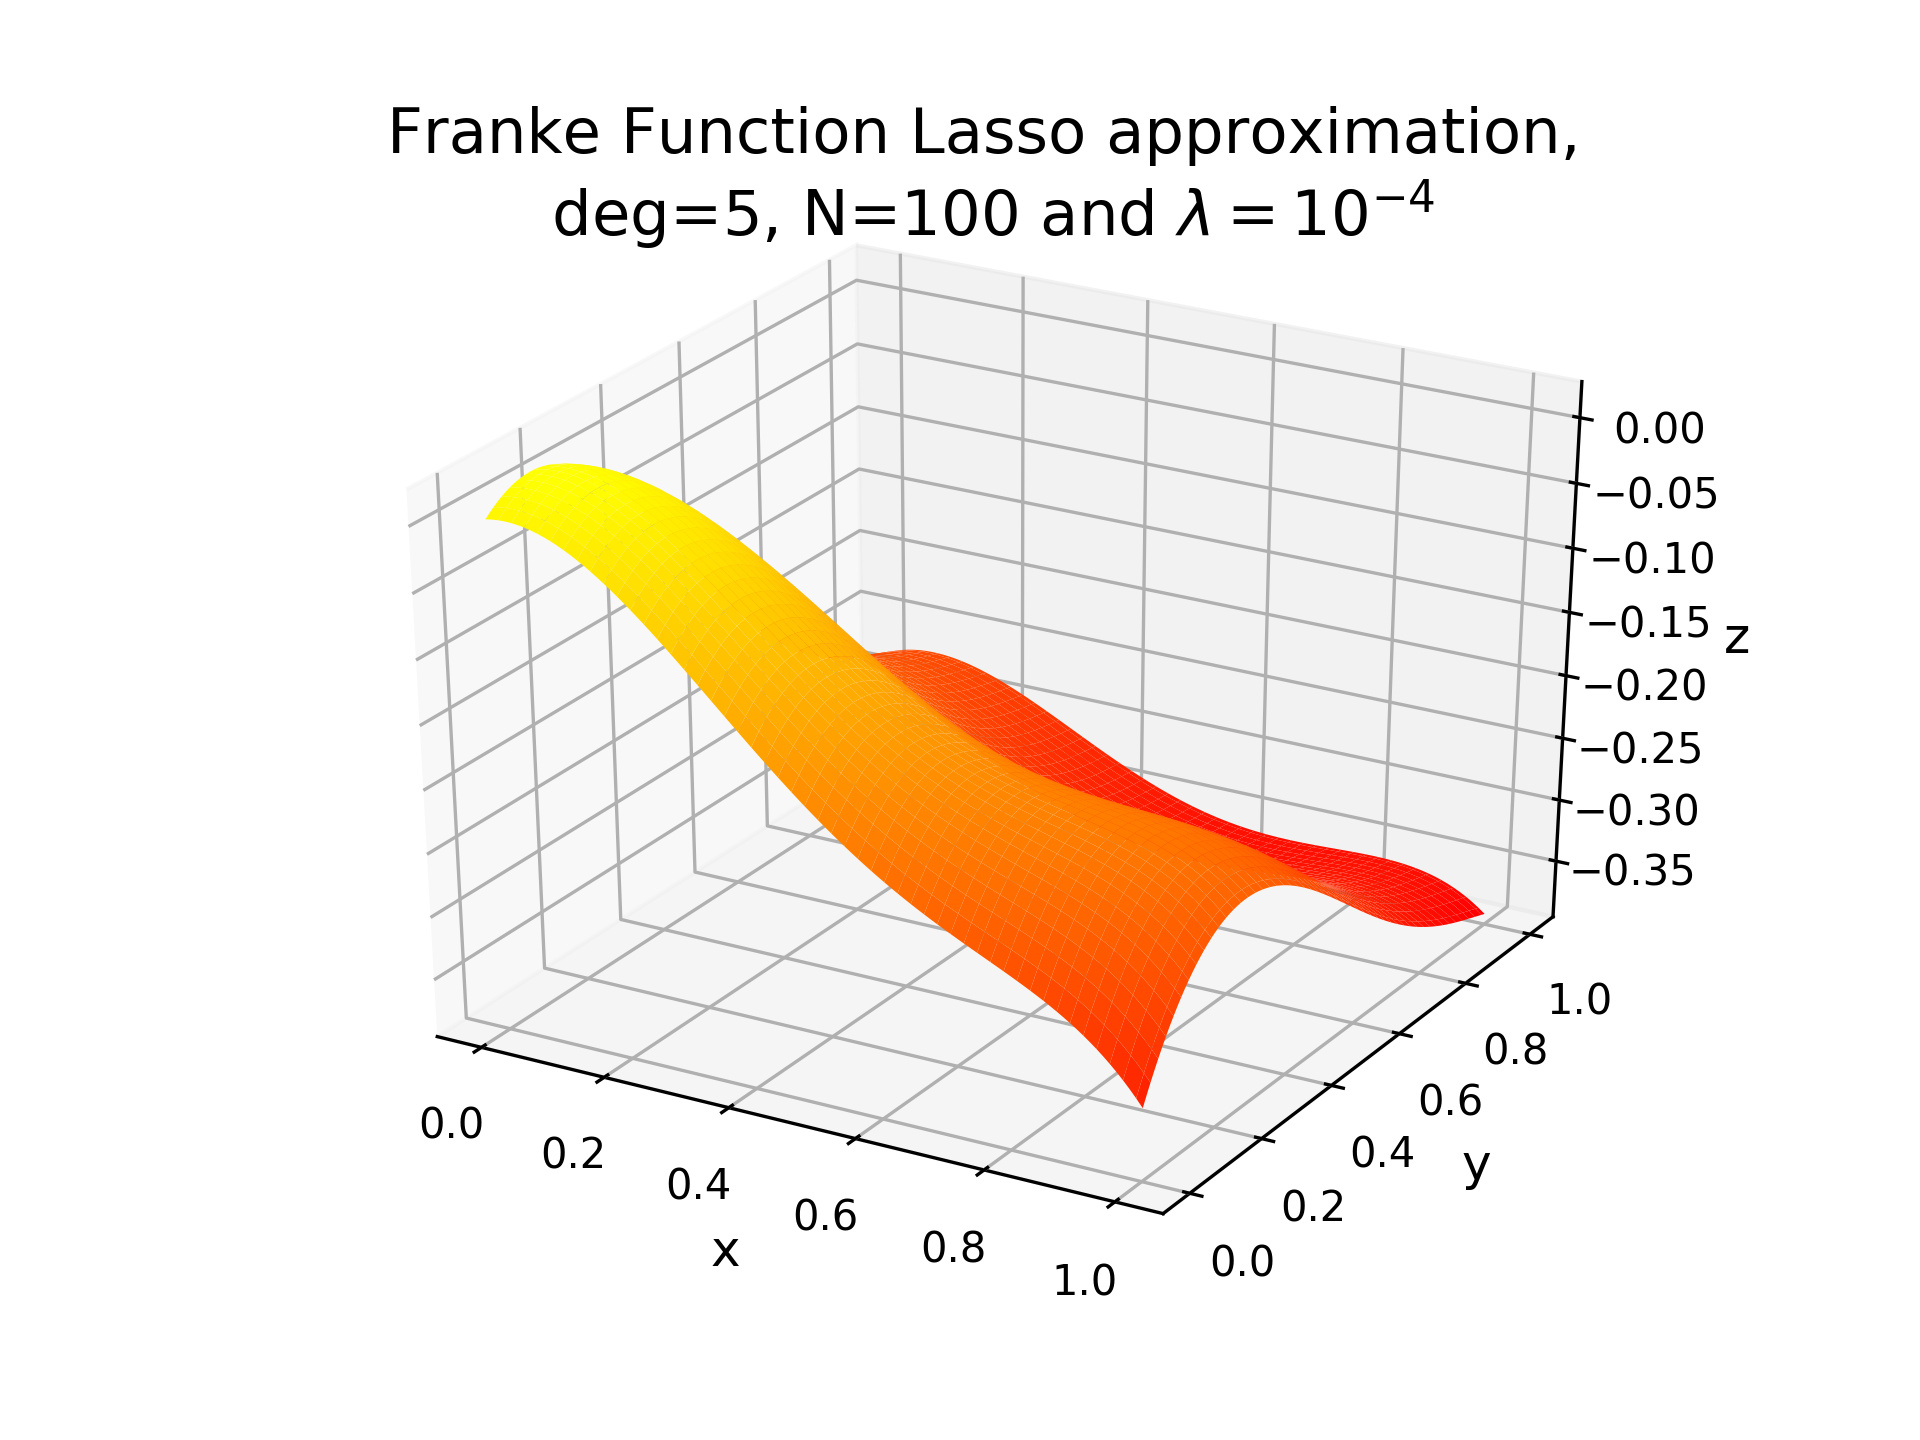
\includegraphics[width=0.45\textwidth]{../Figures/franke_lasso_deg5_N100.png}
  	\caption{Lasso approximation of the Franke function by a 5th degree polynomial using a penalty $\lambda=10^{-4}$.}
	\label{fig12}
\end{figure}

\clearpage

\begin{figure}
 	\centering
  	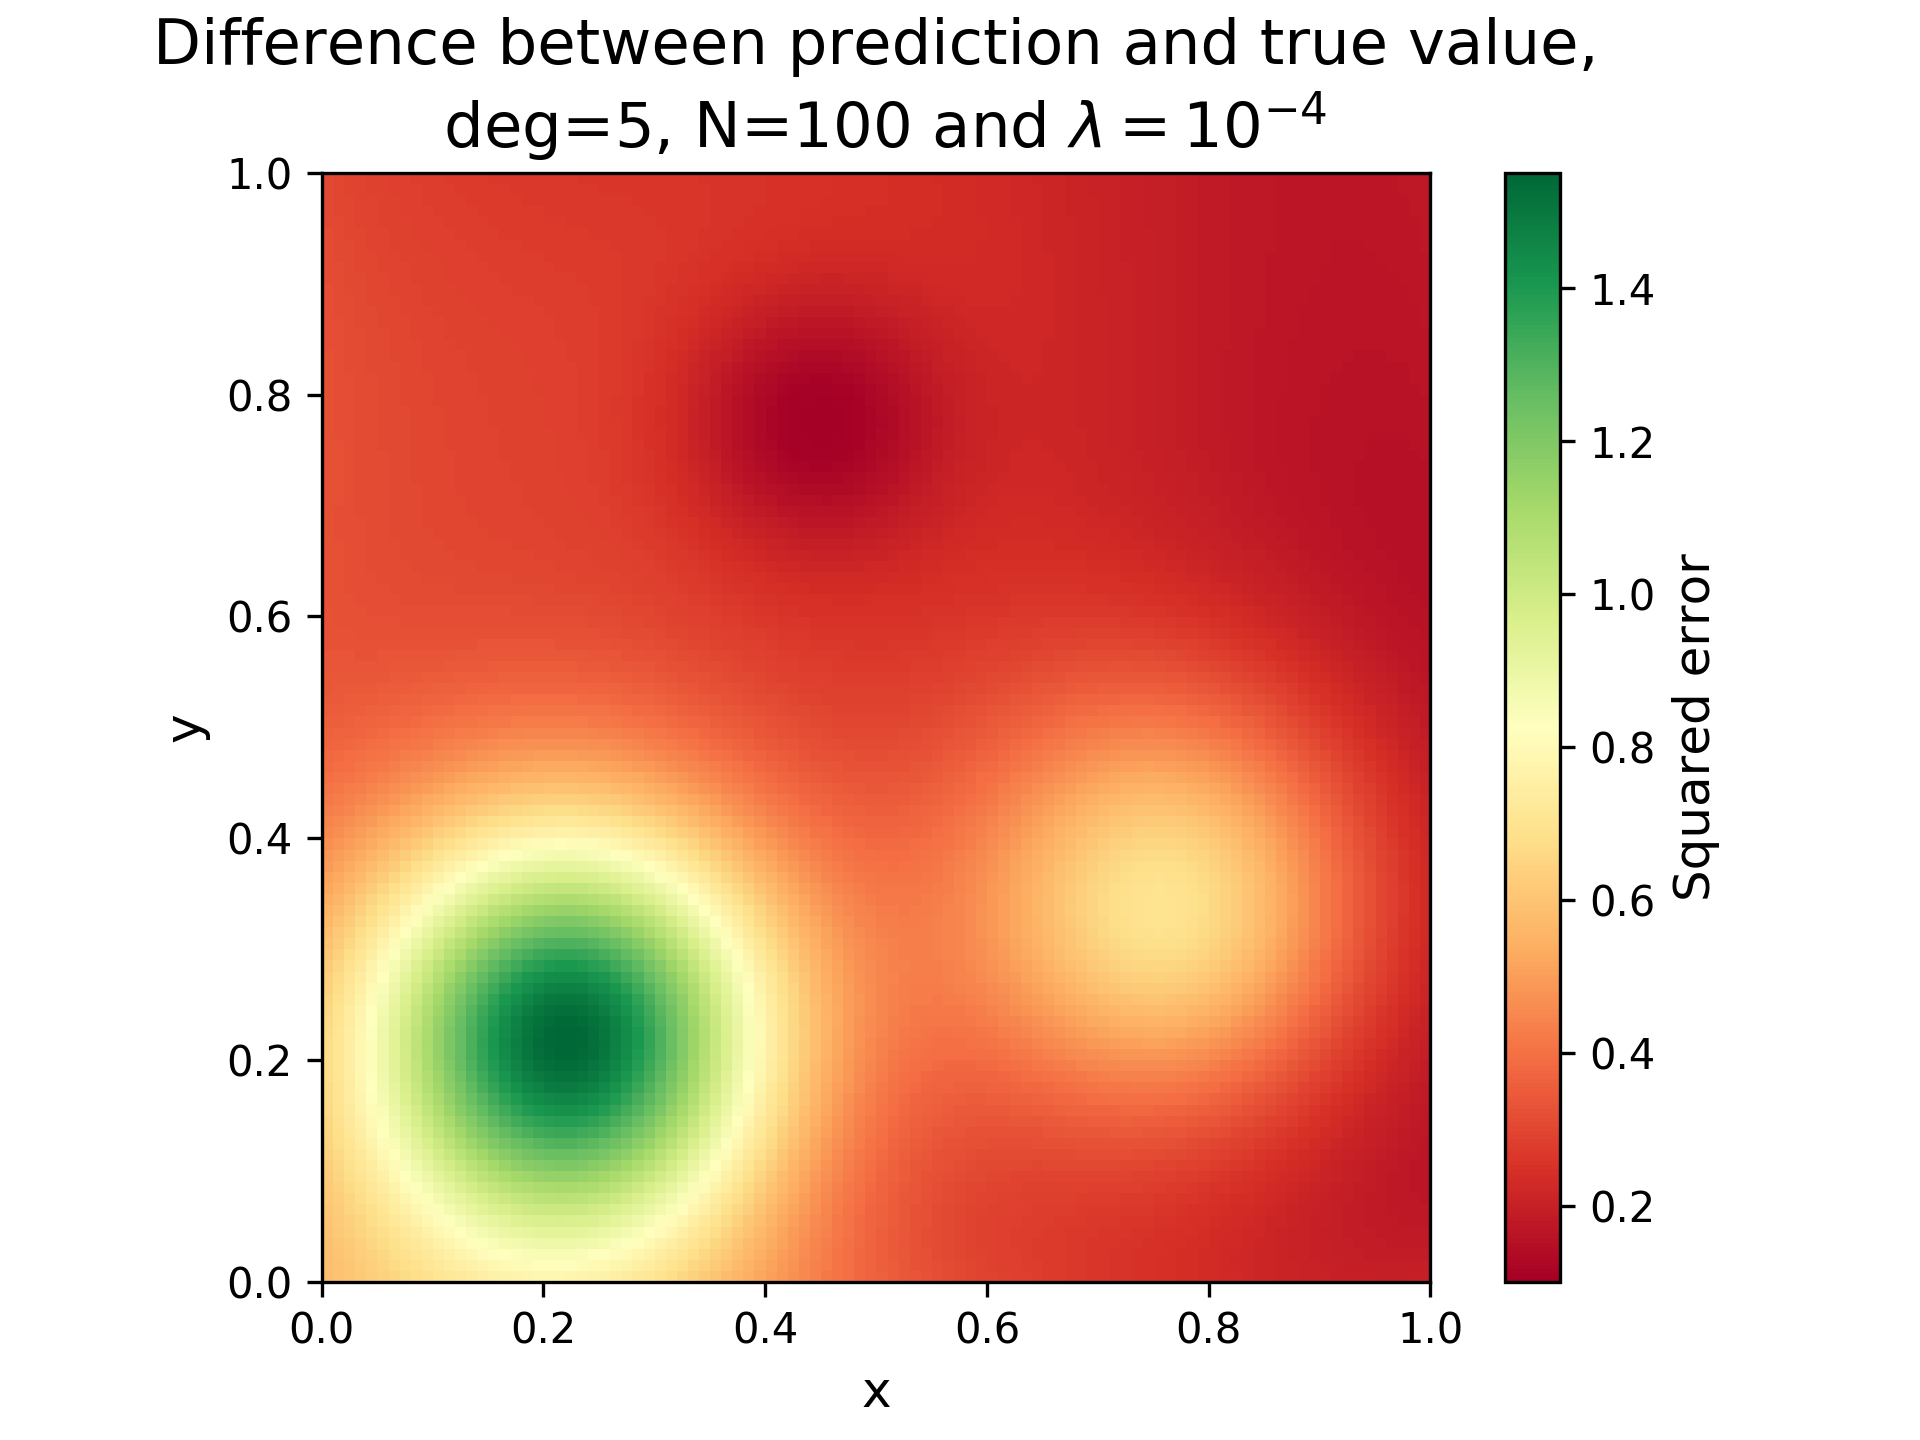
\includegraphics[width=0.45\textwidth]{../Figures/franke_lasso_error_deg5_N100.png}
  	\caption{The errors of the 5th degree lasso approximation of the Franke function with penalty $\lambda=10^{-4}$.}
	\label{fig13}
\end{figure}

% here begins terrain OLS figures

\begin{figure}
	\centering
	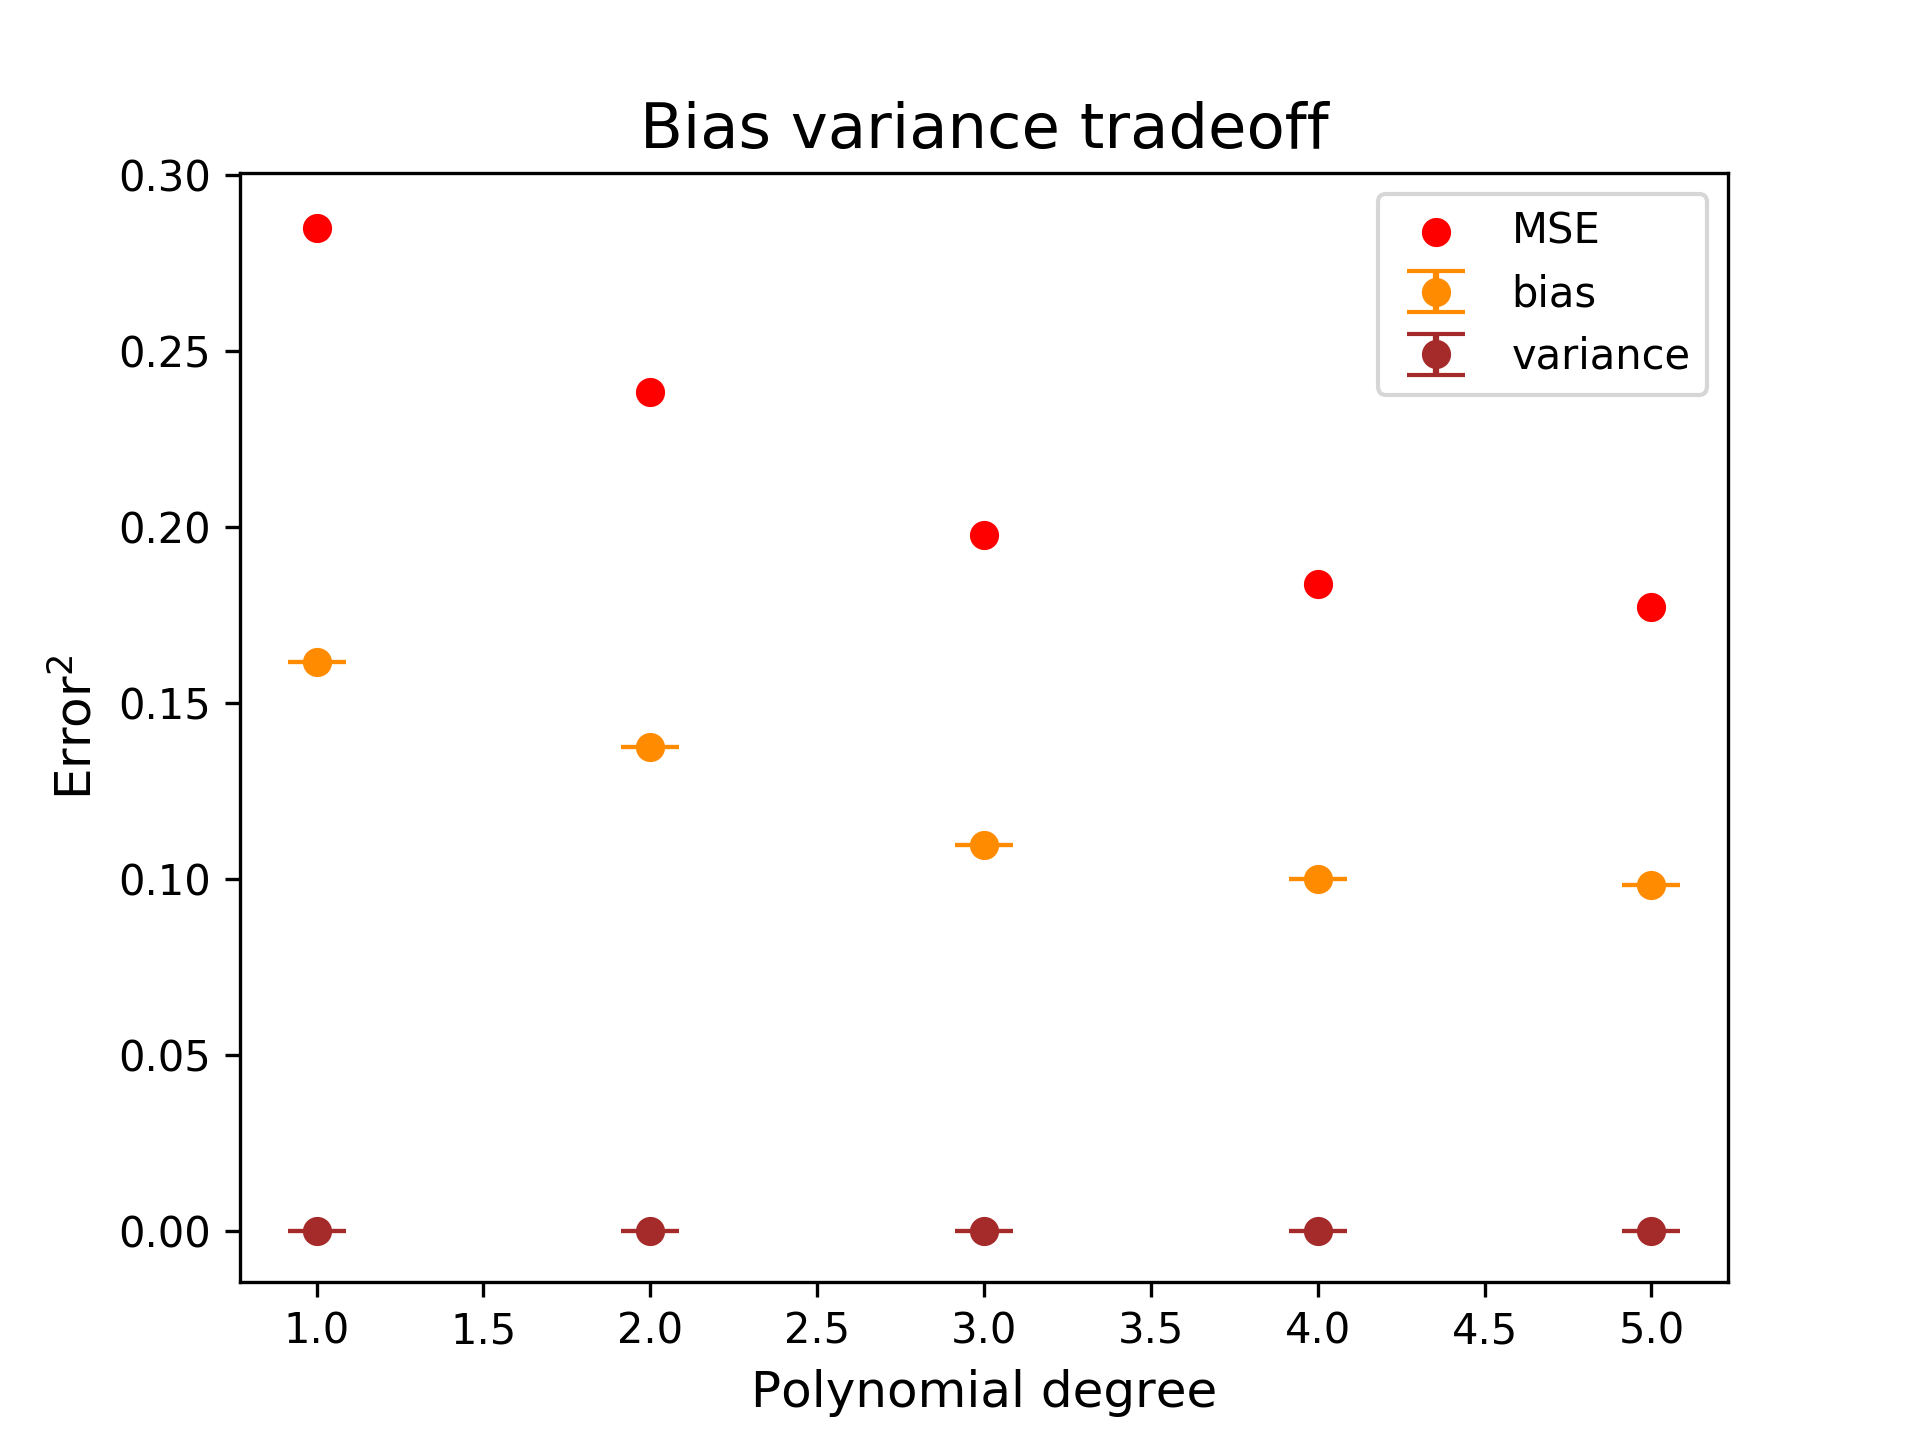
\includegraphics[width=0.45\textwidth]{../Figures/b-v_tradeoff_terrain_OLS.png}
	\caption{Bias variance tradeoff of the terrain data OLS approximation.}
	\label{fig14}
\end{figure}

\begin{figure}
	\centering
	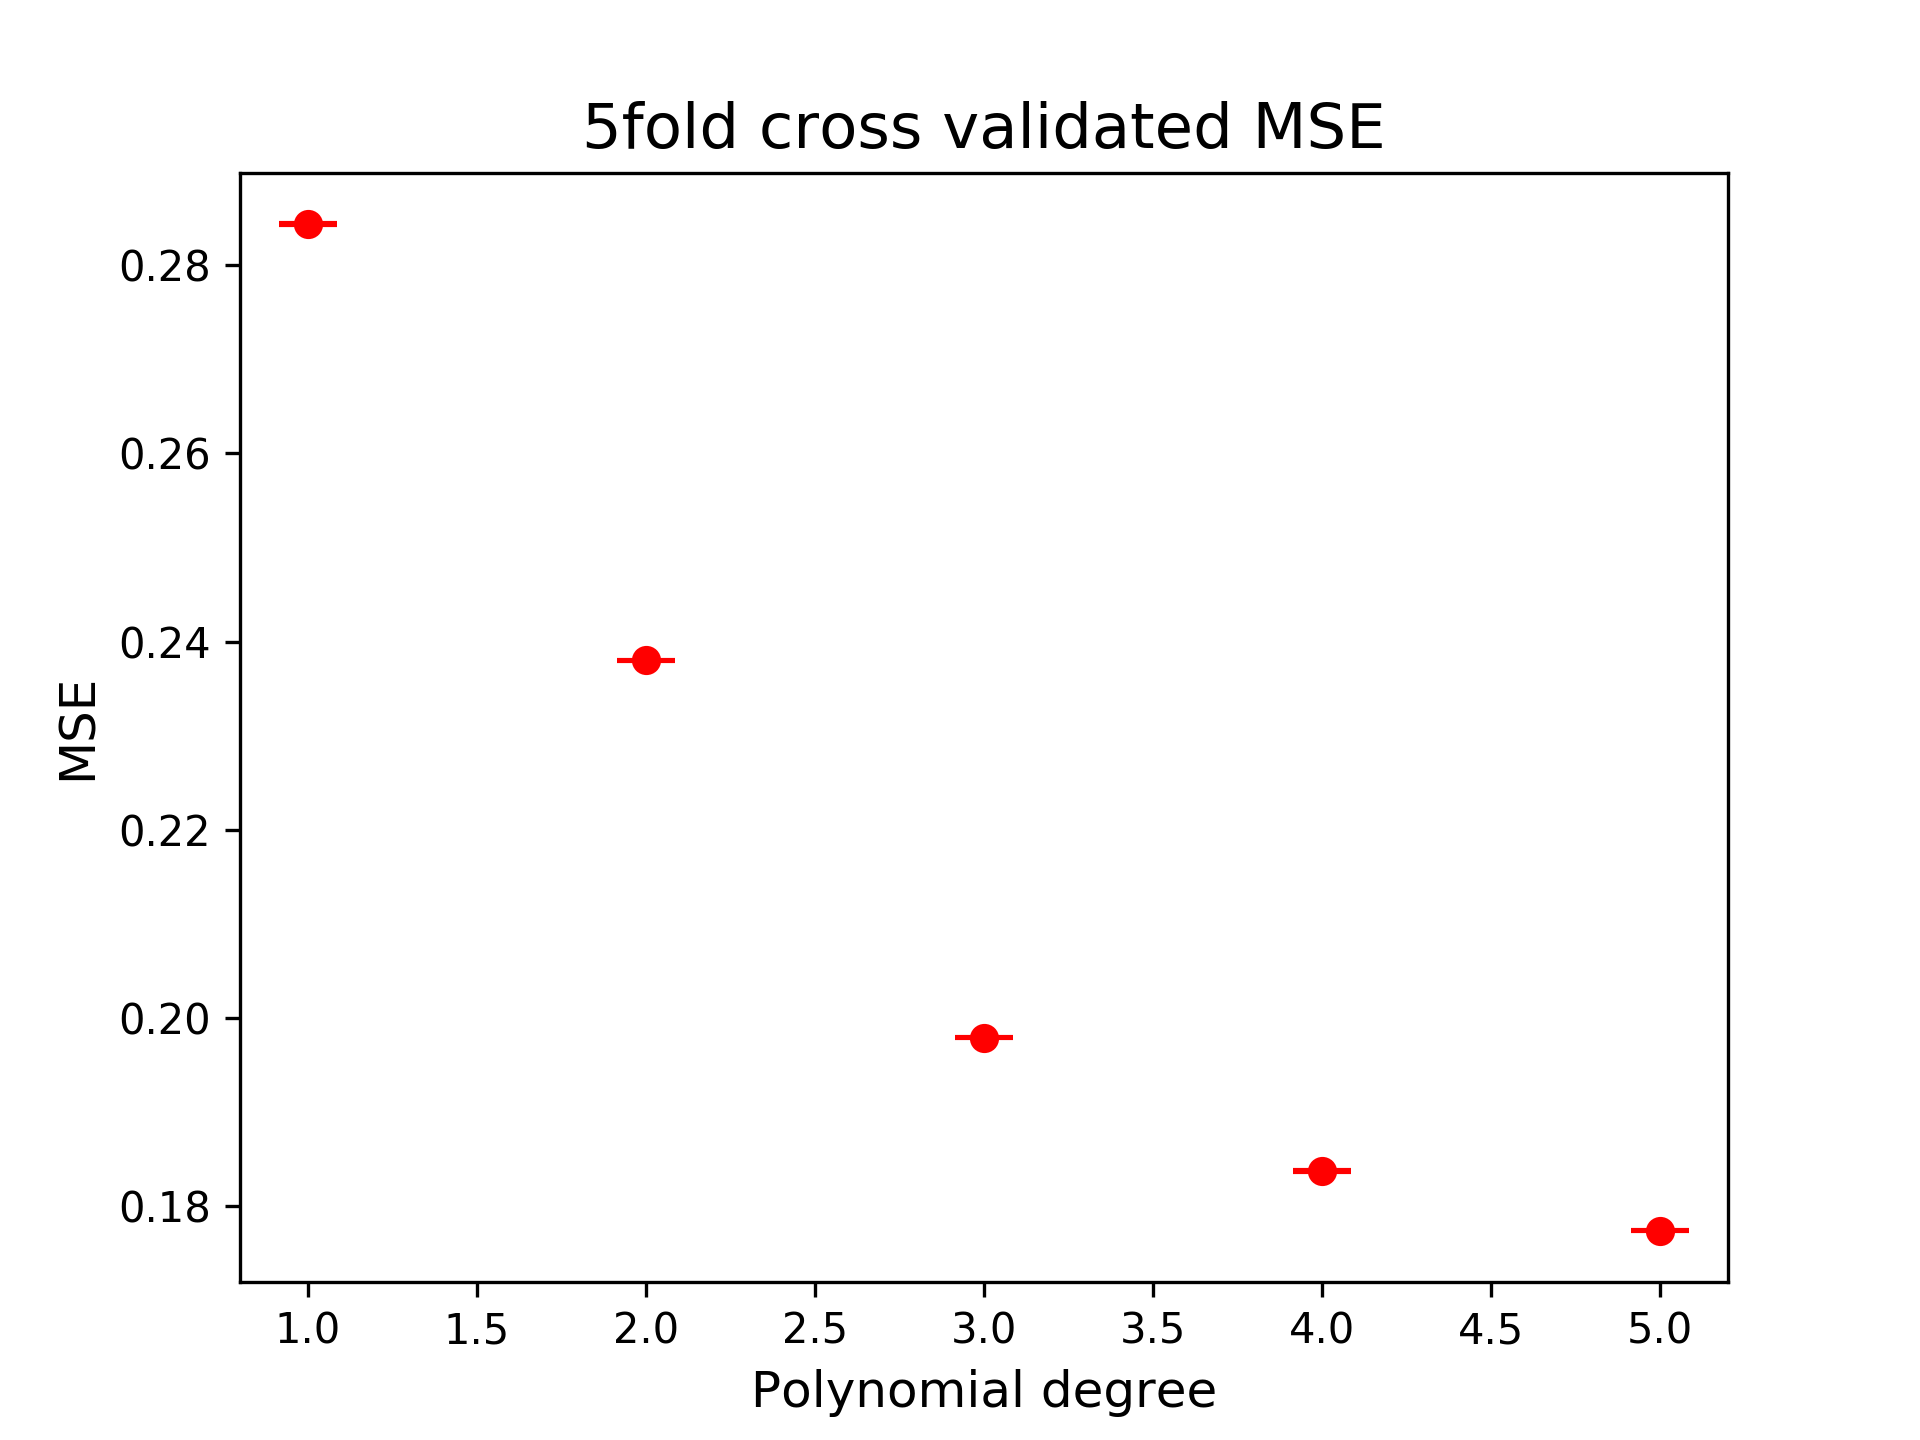
\includegraphics[width=0.45\textwidth]{../Figures/kfold_mse_terrain_OLS.png}
	\caption{Cross validated MSE as a function of model complexity for the terrain data OLS approximation.}
	\label{fig15}
\end{figure}

\begin{figure}
 	\centering
	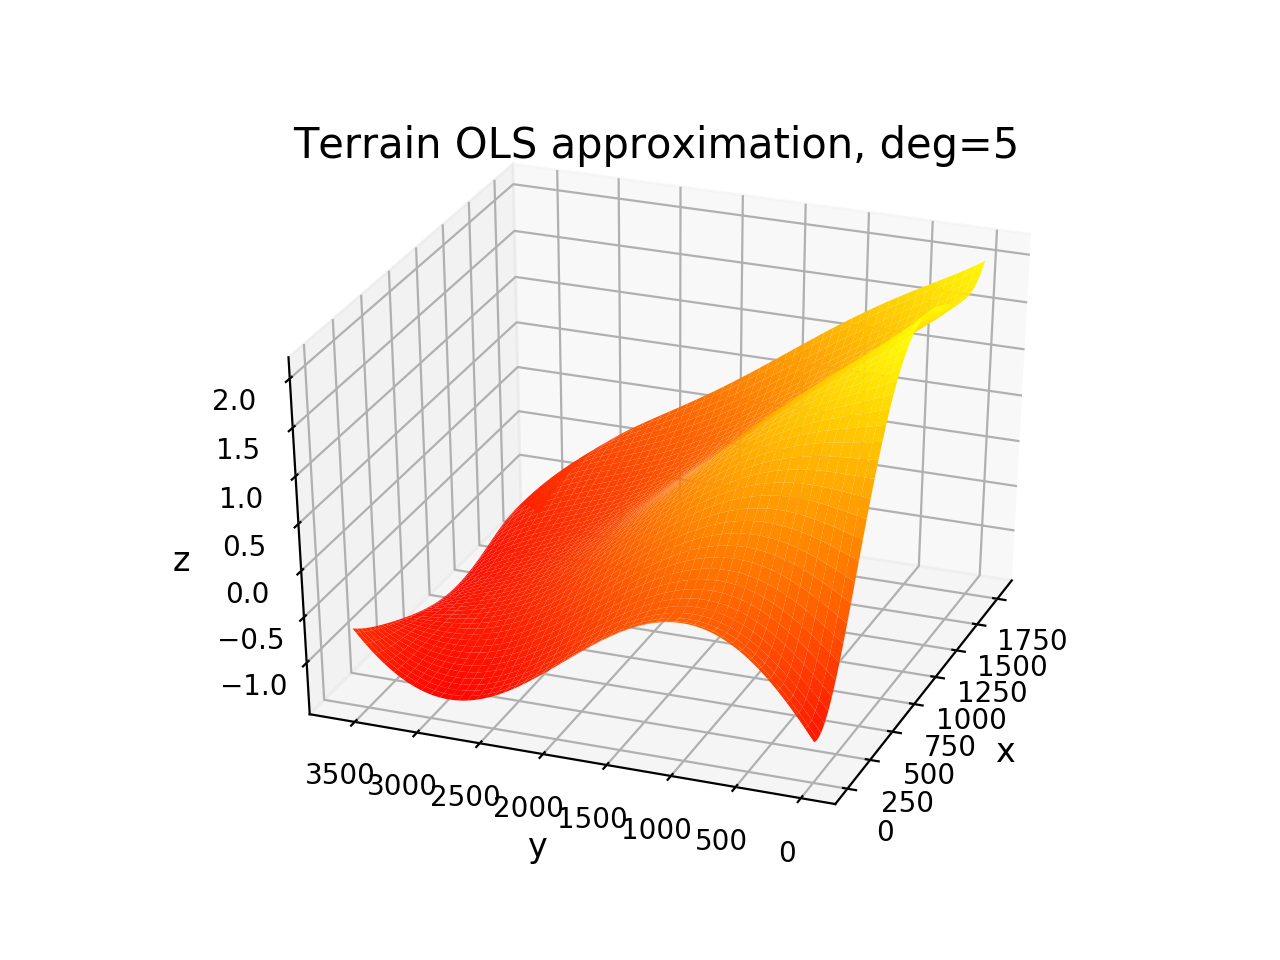
\includegraphics[width=0.45\textwidth]{../Figures/terrain_OLS_deg5_adjusted.png}
  	\caption{OLS approximation of the terrain data by a 5th degree polynomial.}
	\label{fig16}
\end{figure}

\begin{figure}
 	\centering
  	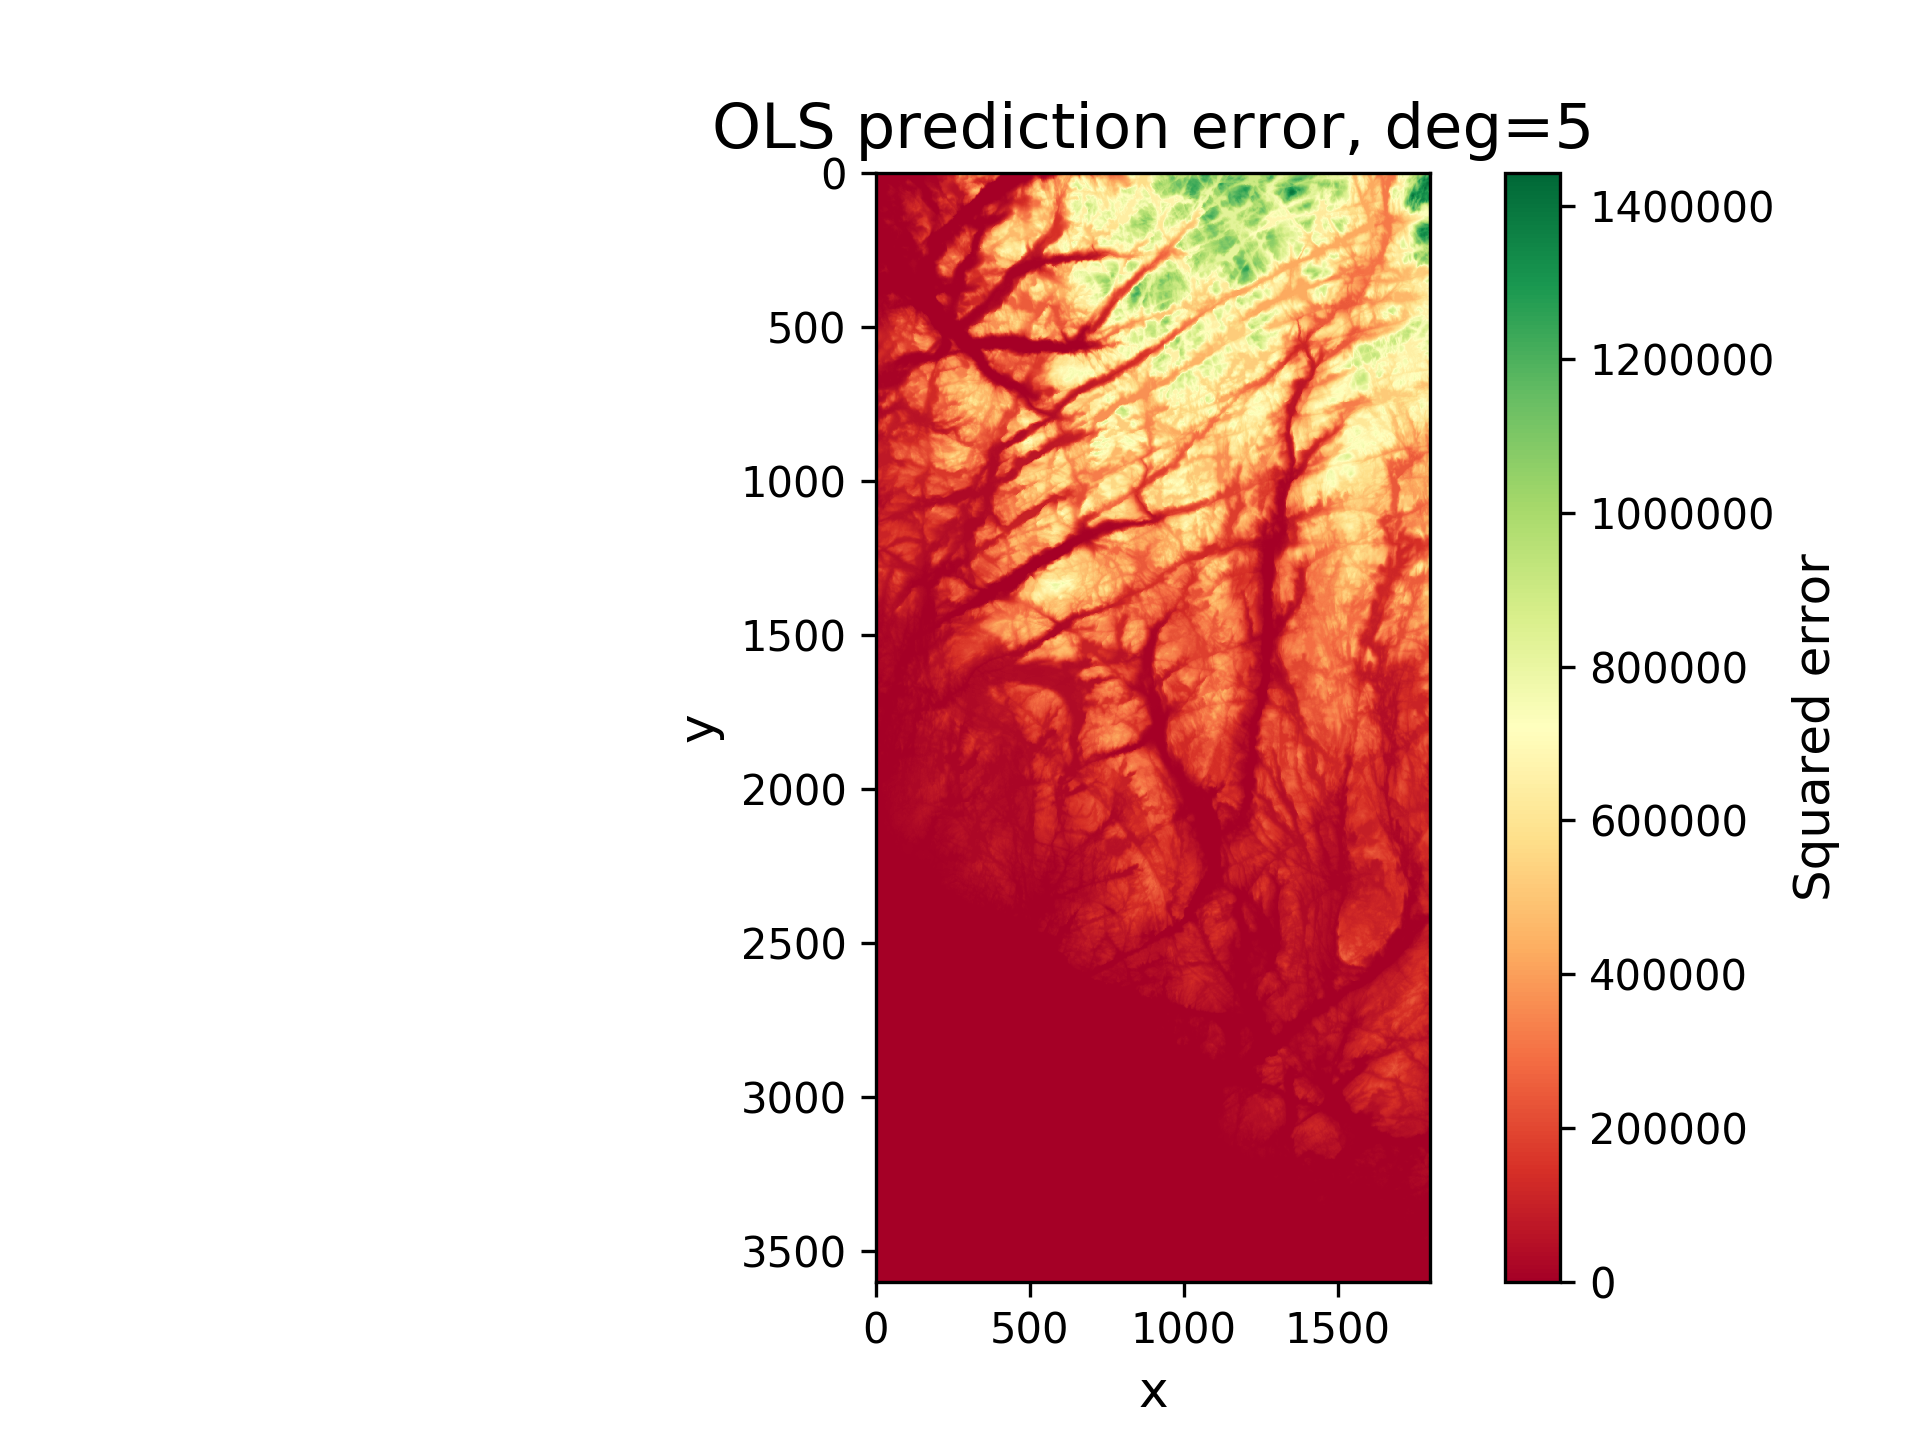
\includegraphics[width=0.45\textwidth]{../Figures/terrain_OLS_error_deg5.png}
  	\caption{The errors of the 5th degree OLS approximation of the terrain data.}
	\label{fig17}
\end{figure}

% here begins terrain ridge figures

\begin{figure}
	\centering
	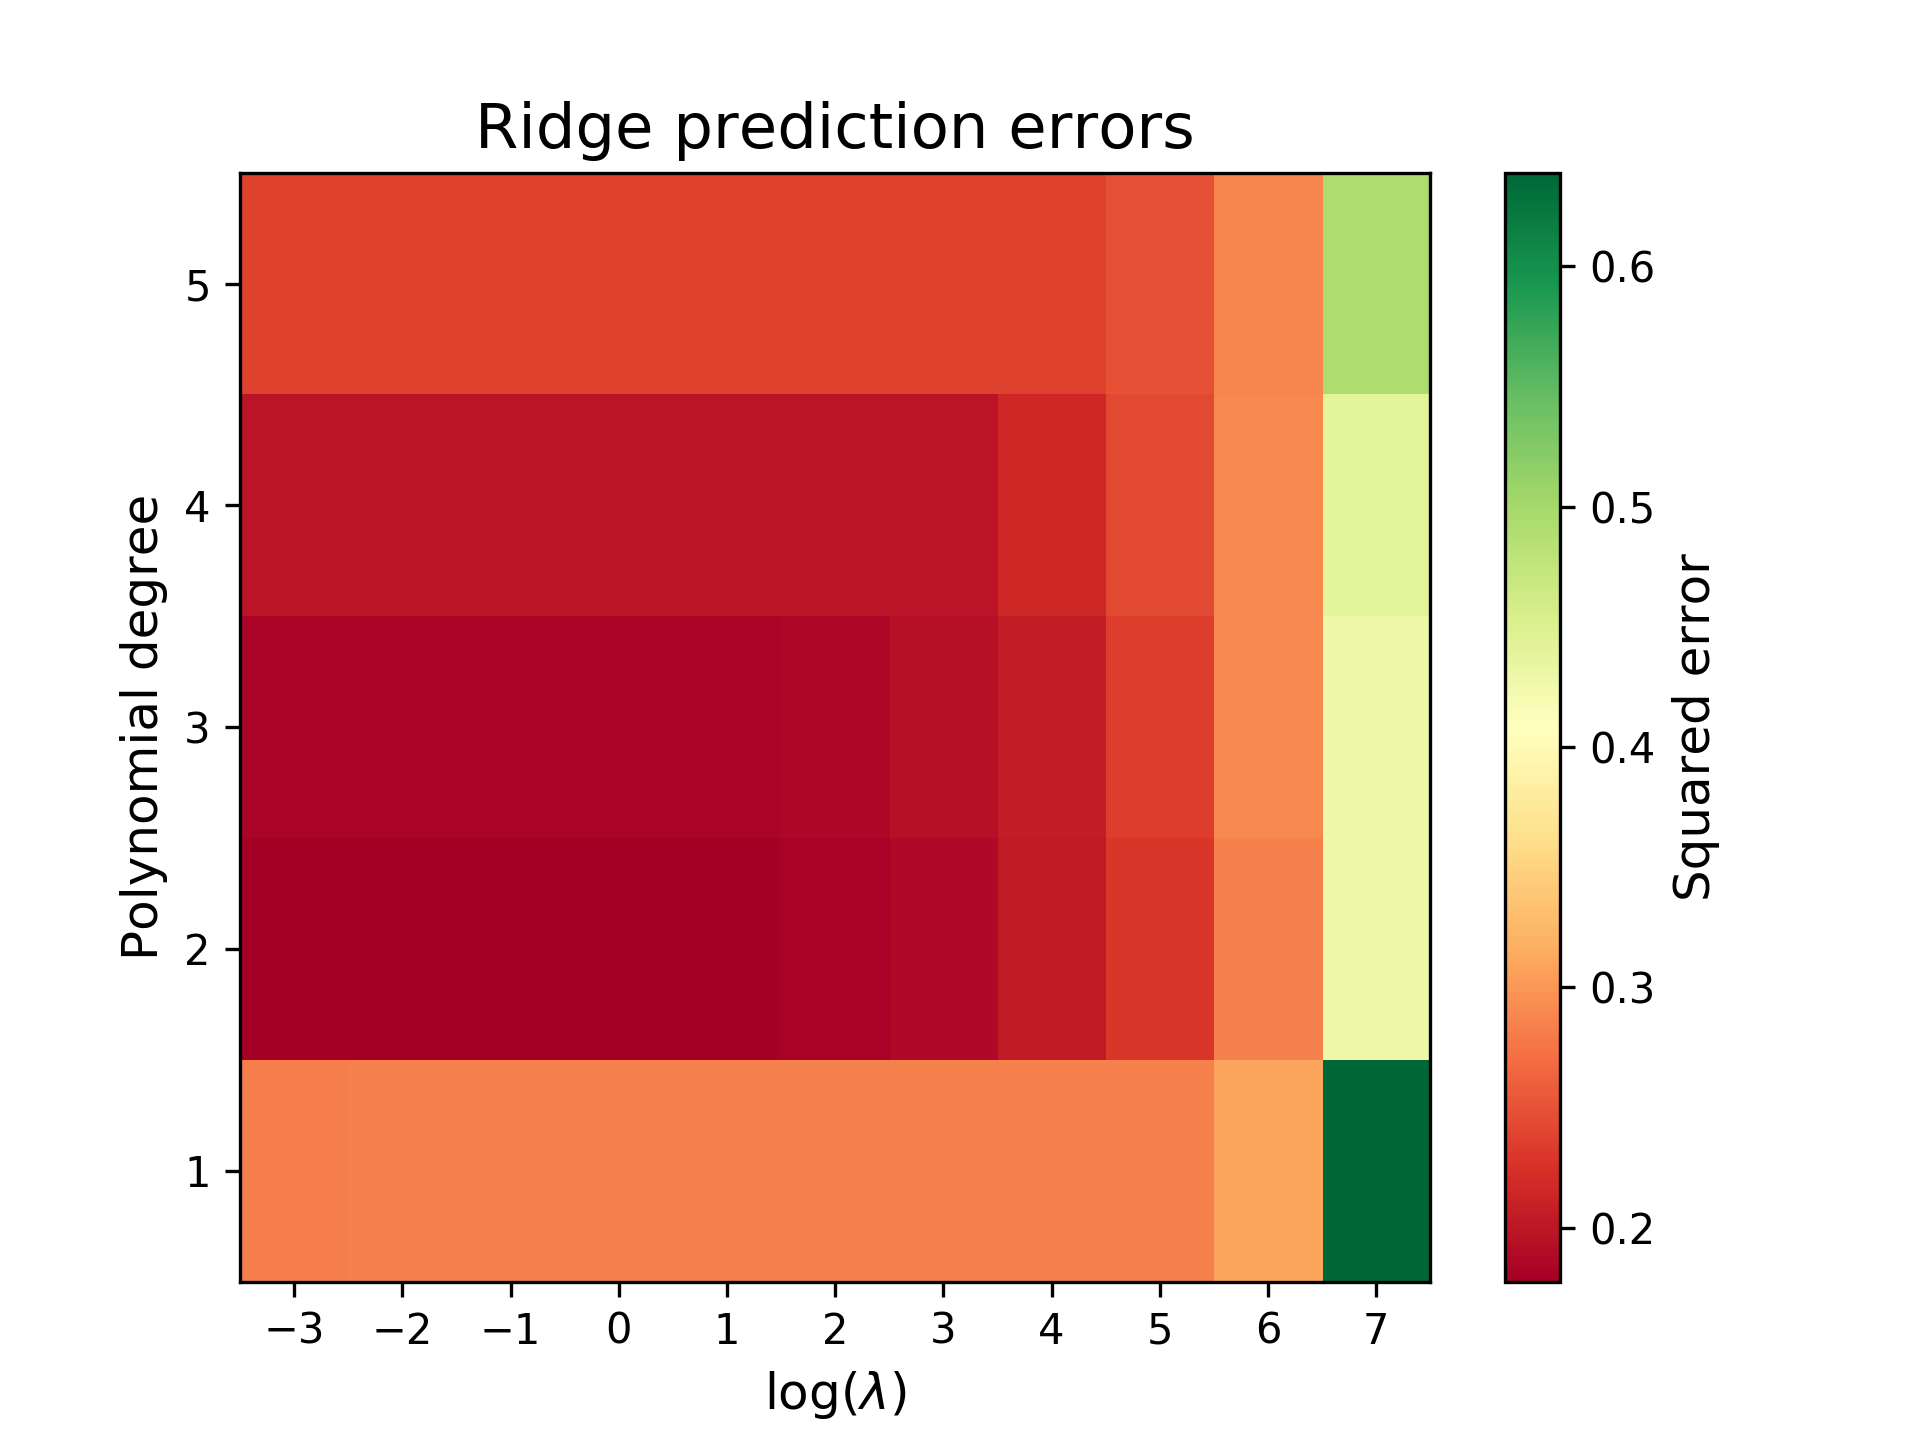
\includegraphics[width=0.45\textwidth]{../Figures/ridge_grid_search.png}
	\caption{The test MSE for each combination of penalties $\lambda$ and polynomial degrees for ridge regression of terrain data.}
	\label{fig18}
\end{figure}

\clearpage

\begin{figure}
	\centering
	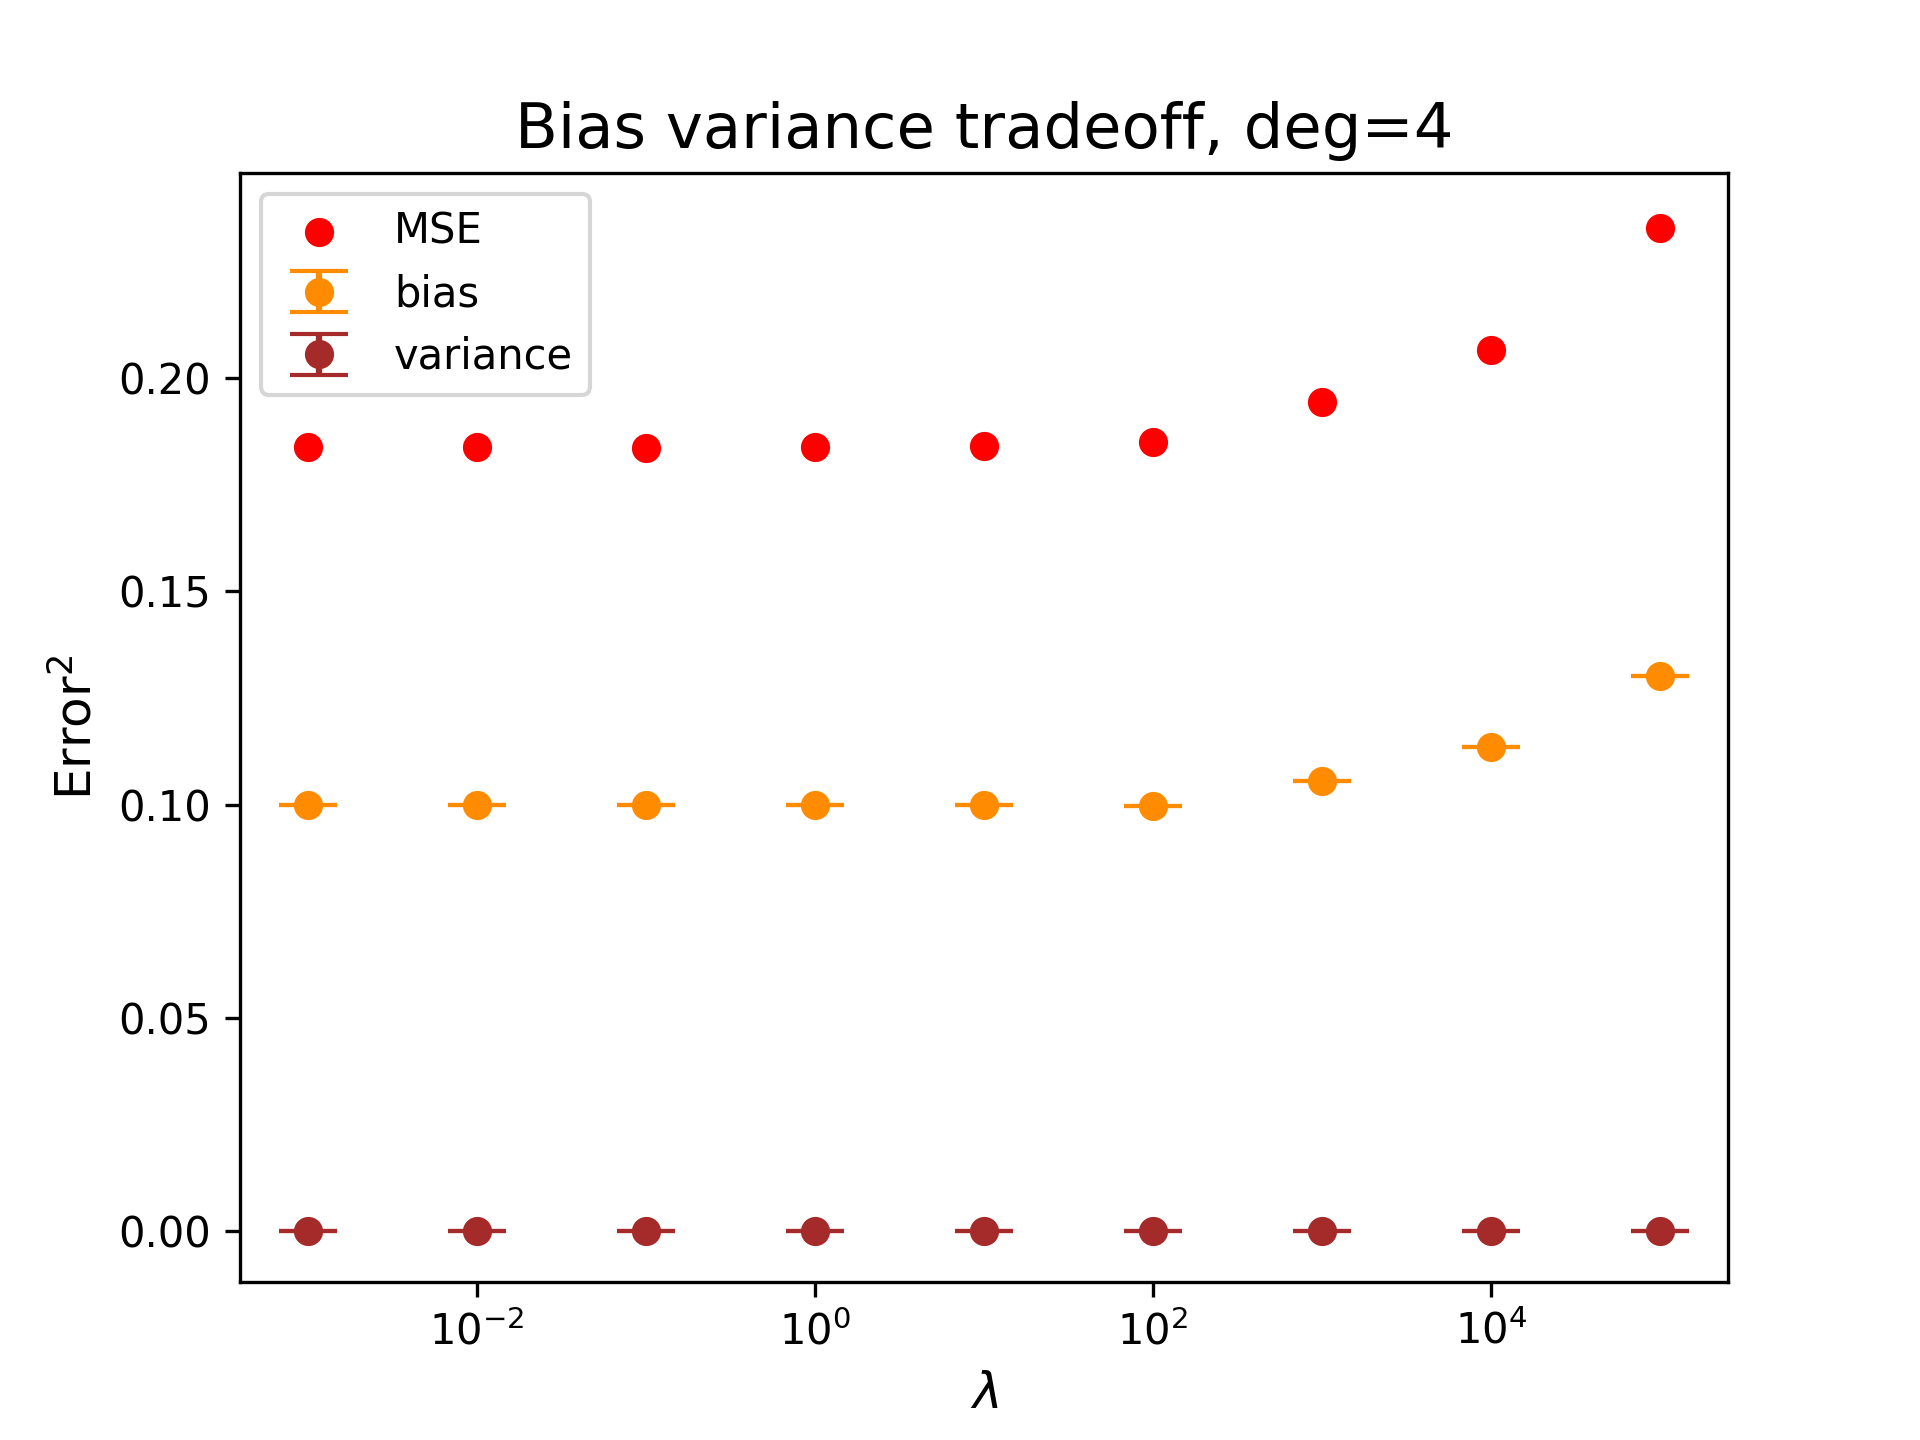
\includegraphics[width=0.45\textwidth]{../Figures/b-v_tradeoff_terrain_ridge_deg4.png}
	\caption{Bias variance tradeoff for a 4th degree ridge approximation on terrain data.}
	\label{fig19}
\end{figure}

\begin{figure}
	\centering
	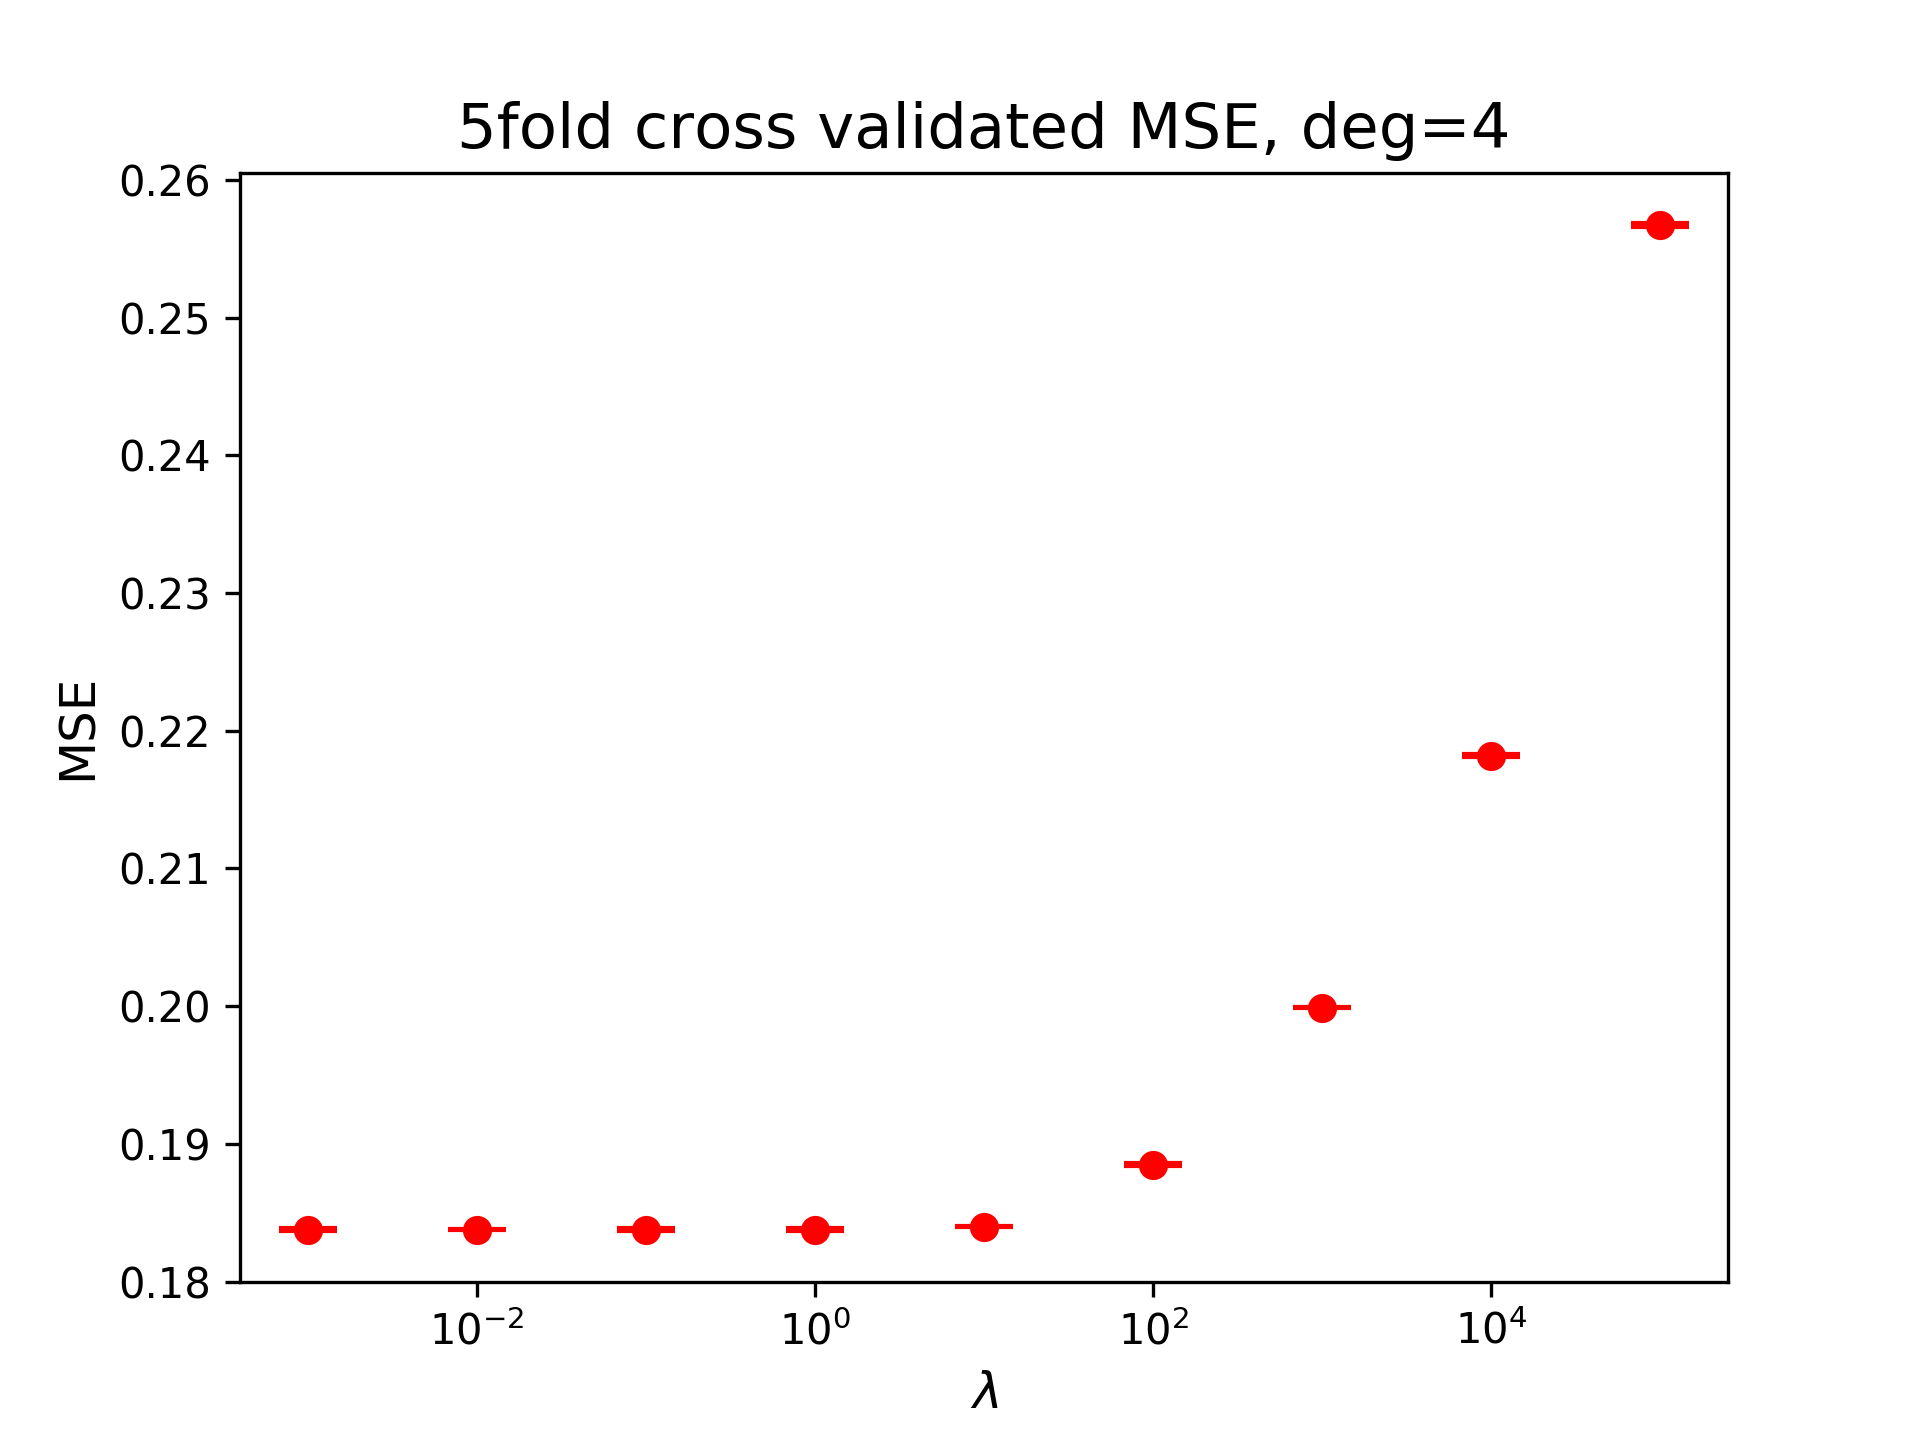
\includegraphics[width=0.45\textwidth]{../Figures/kfold_mse_terrain_ridge_deg4.png}
	\caption{5fold cross validation of penalties $\lambda$ for a 4th degree ridge approximation on terrain data.}
	\label{fig20}
\end{figure}

\begin{figure}
	\centering
	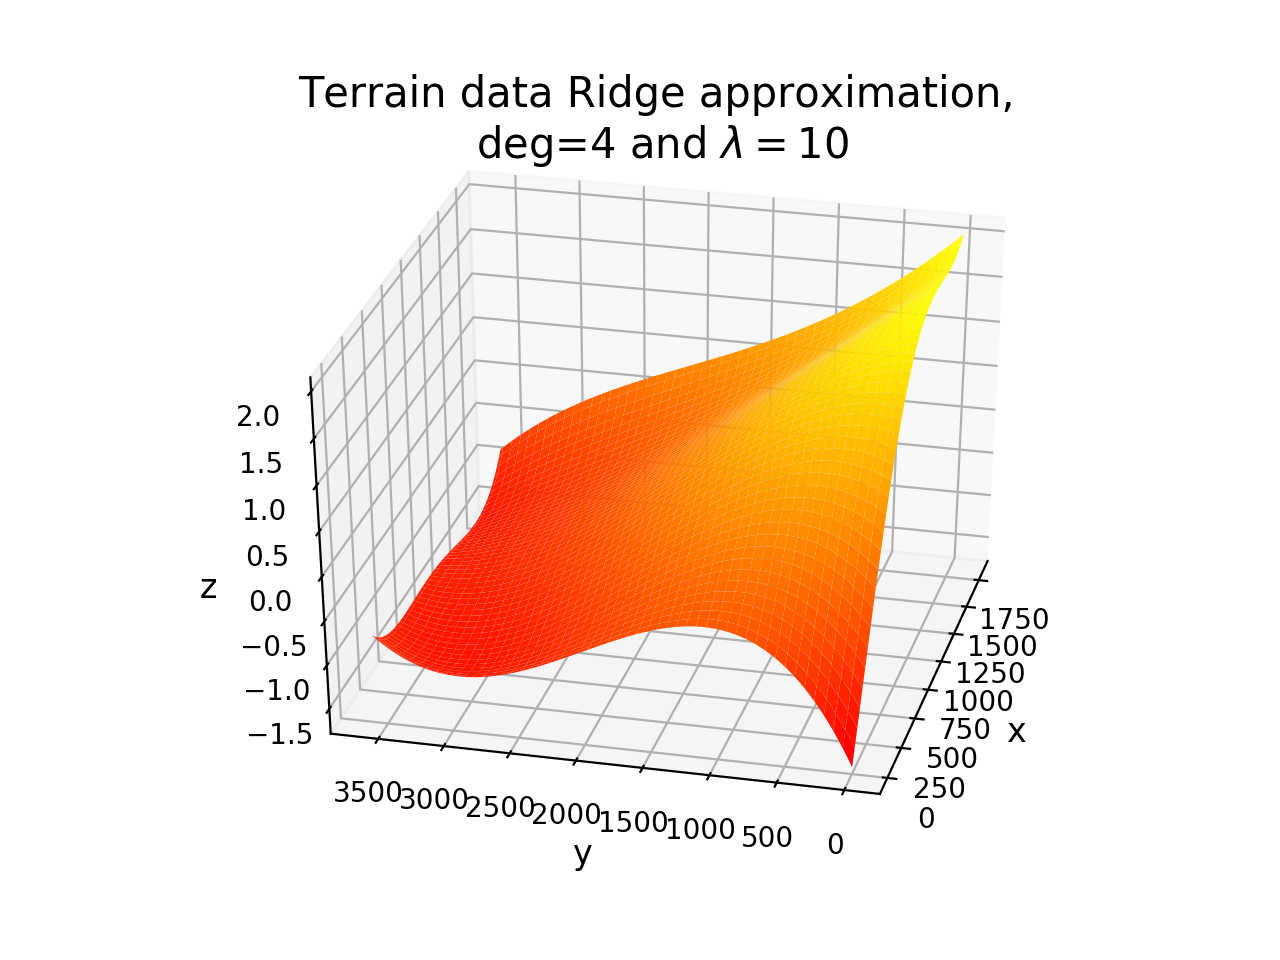
\includegraphics[width=0.45\textwidth]{../Figures/terrain_ridge_deg4_adjusted.png}
	\caption{4th degree ridge approximation of terrain data with penalty $\lambda=10$.}
	\label{fig21}
\end{figure}

\begin{figure}
	\centering
	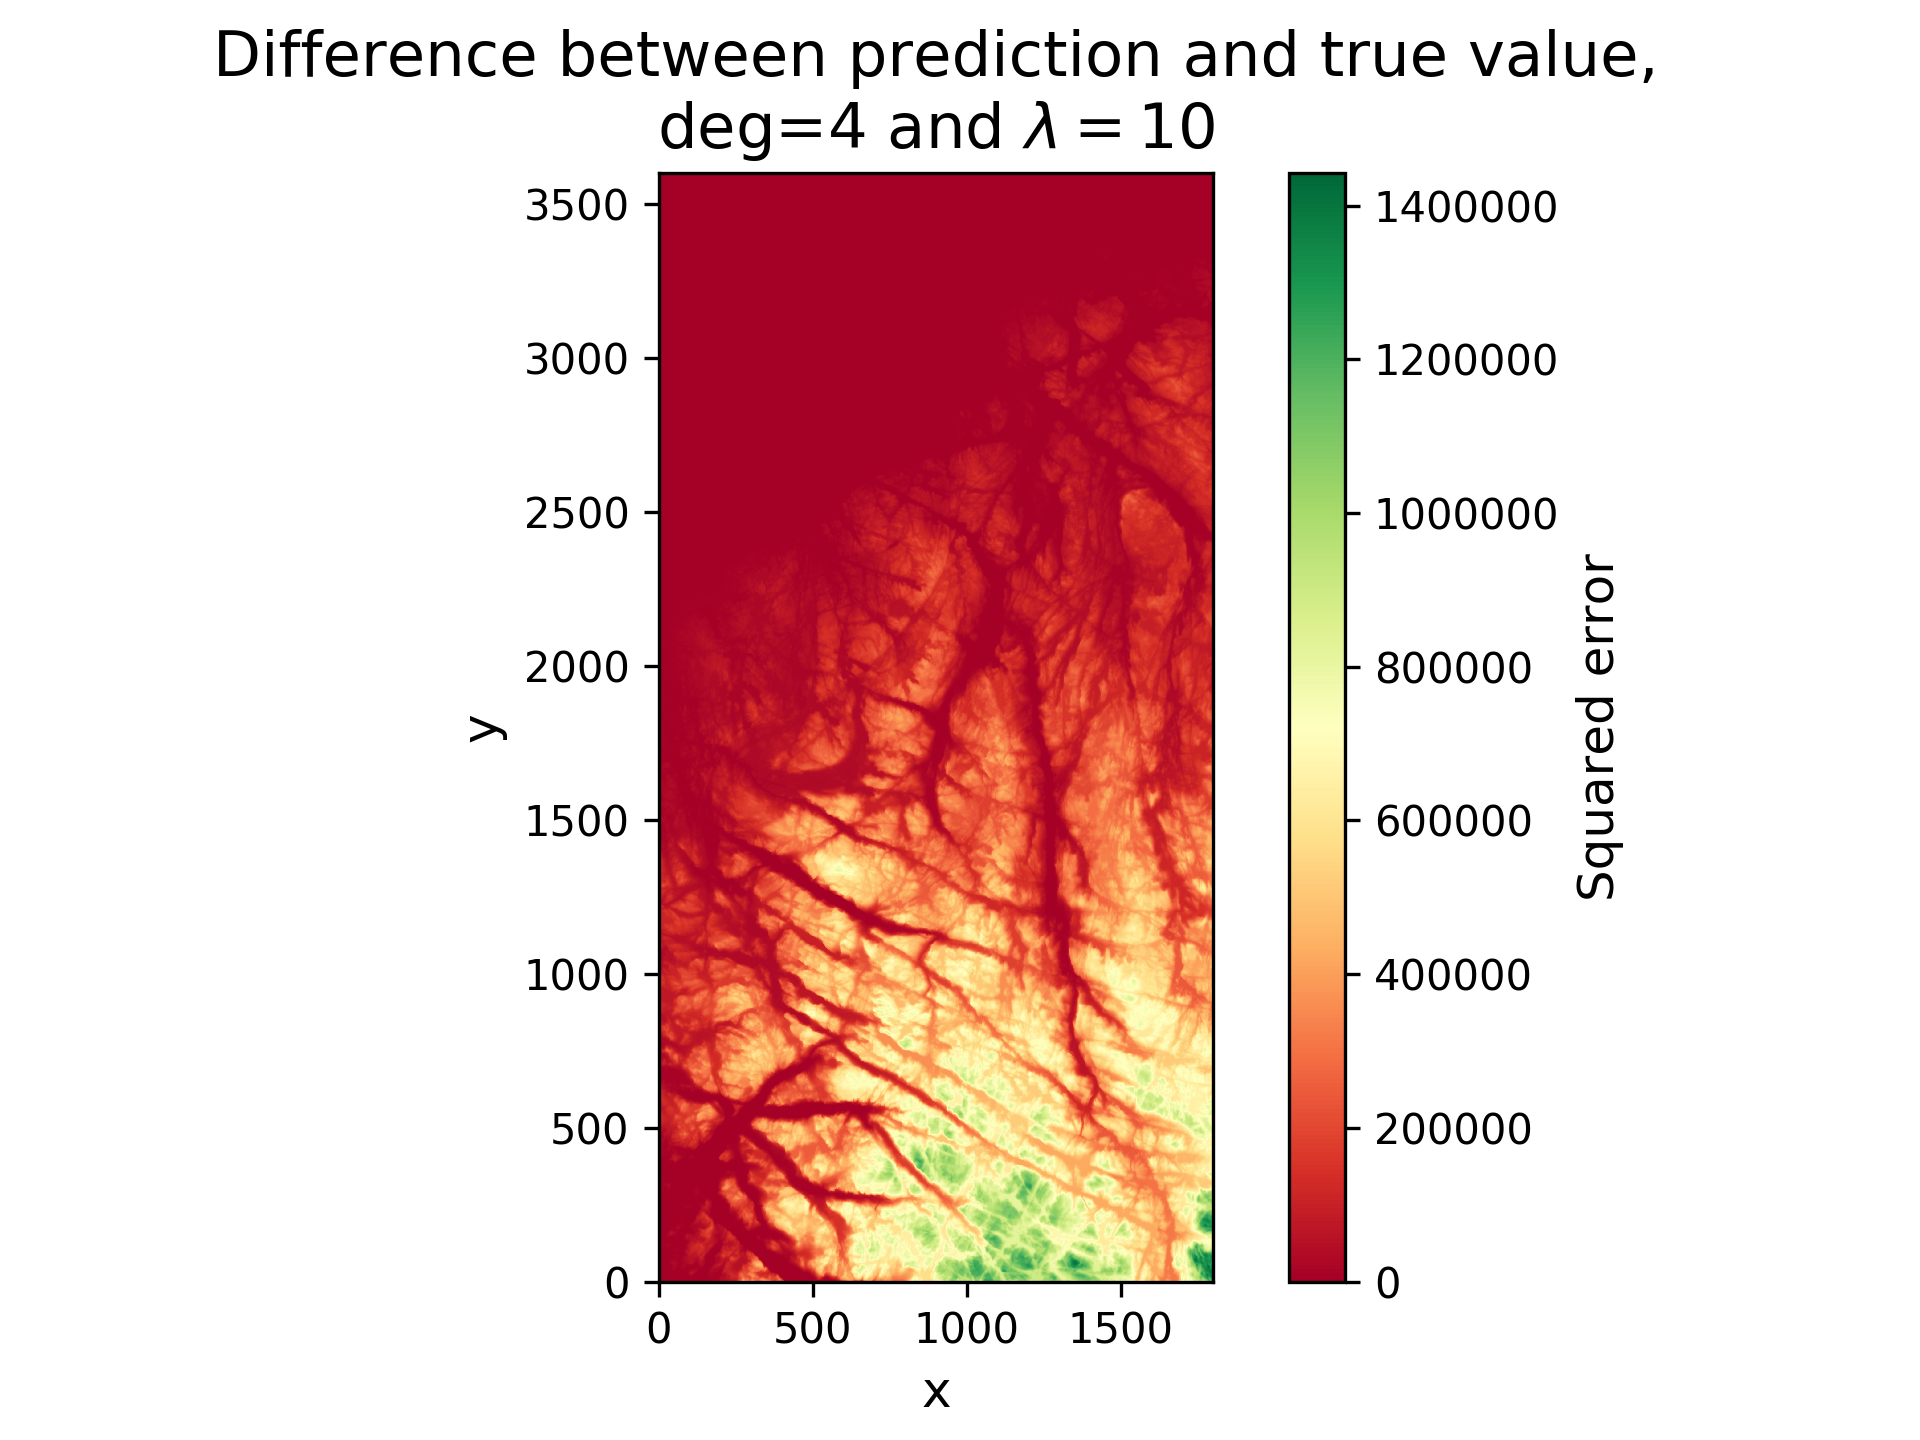
\includegraphics[width=0.45\textwidth]{../Figures/terrain_ridge_error_deg4.png}
	\caption{Errors of the 4th degree ridge approximation of terrain data with penalty $\lambda=10$.}
	\label{fig22}
\end{figure}

% here begins terrain lasso figures 

\begin{figure}
	\centering
	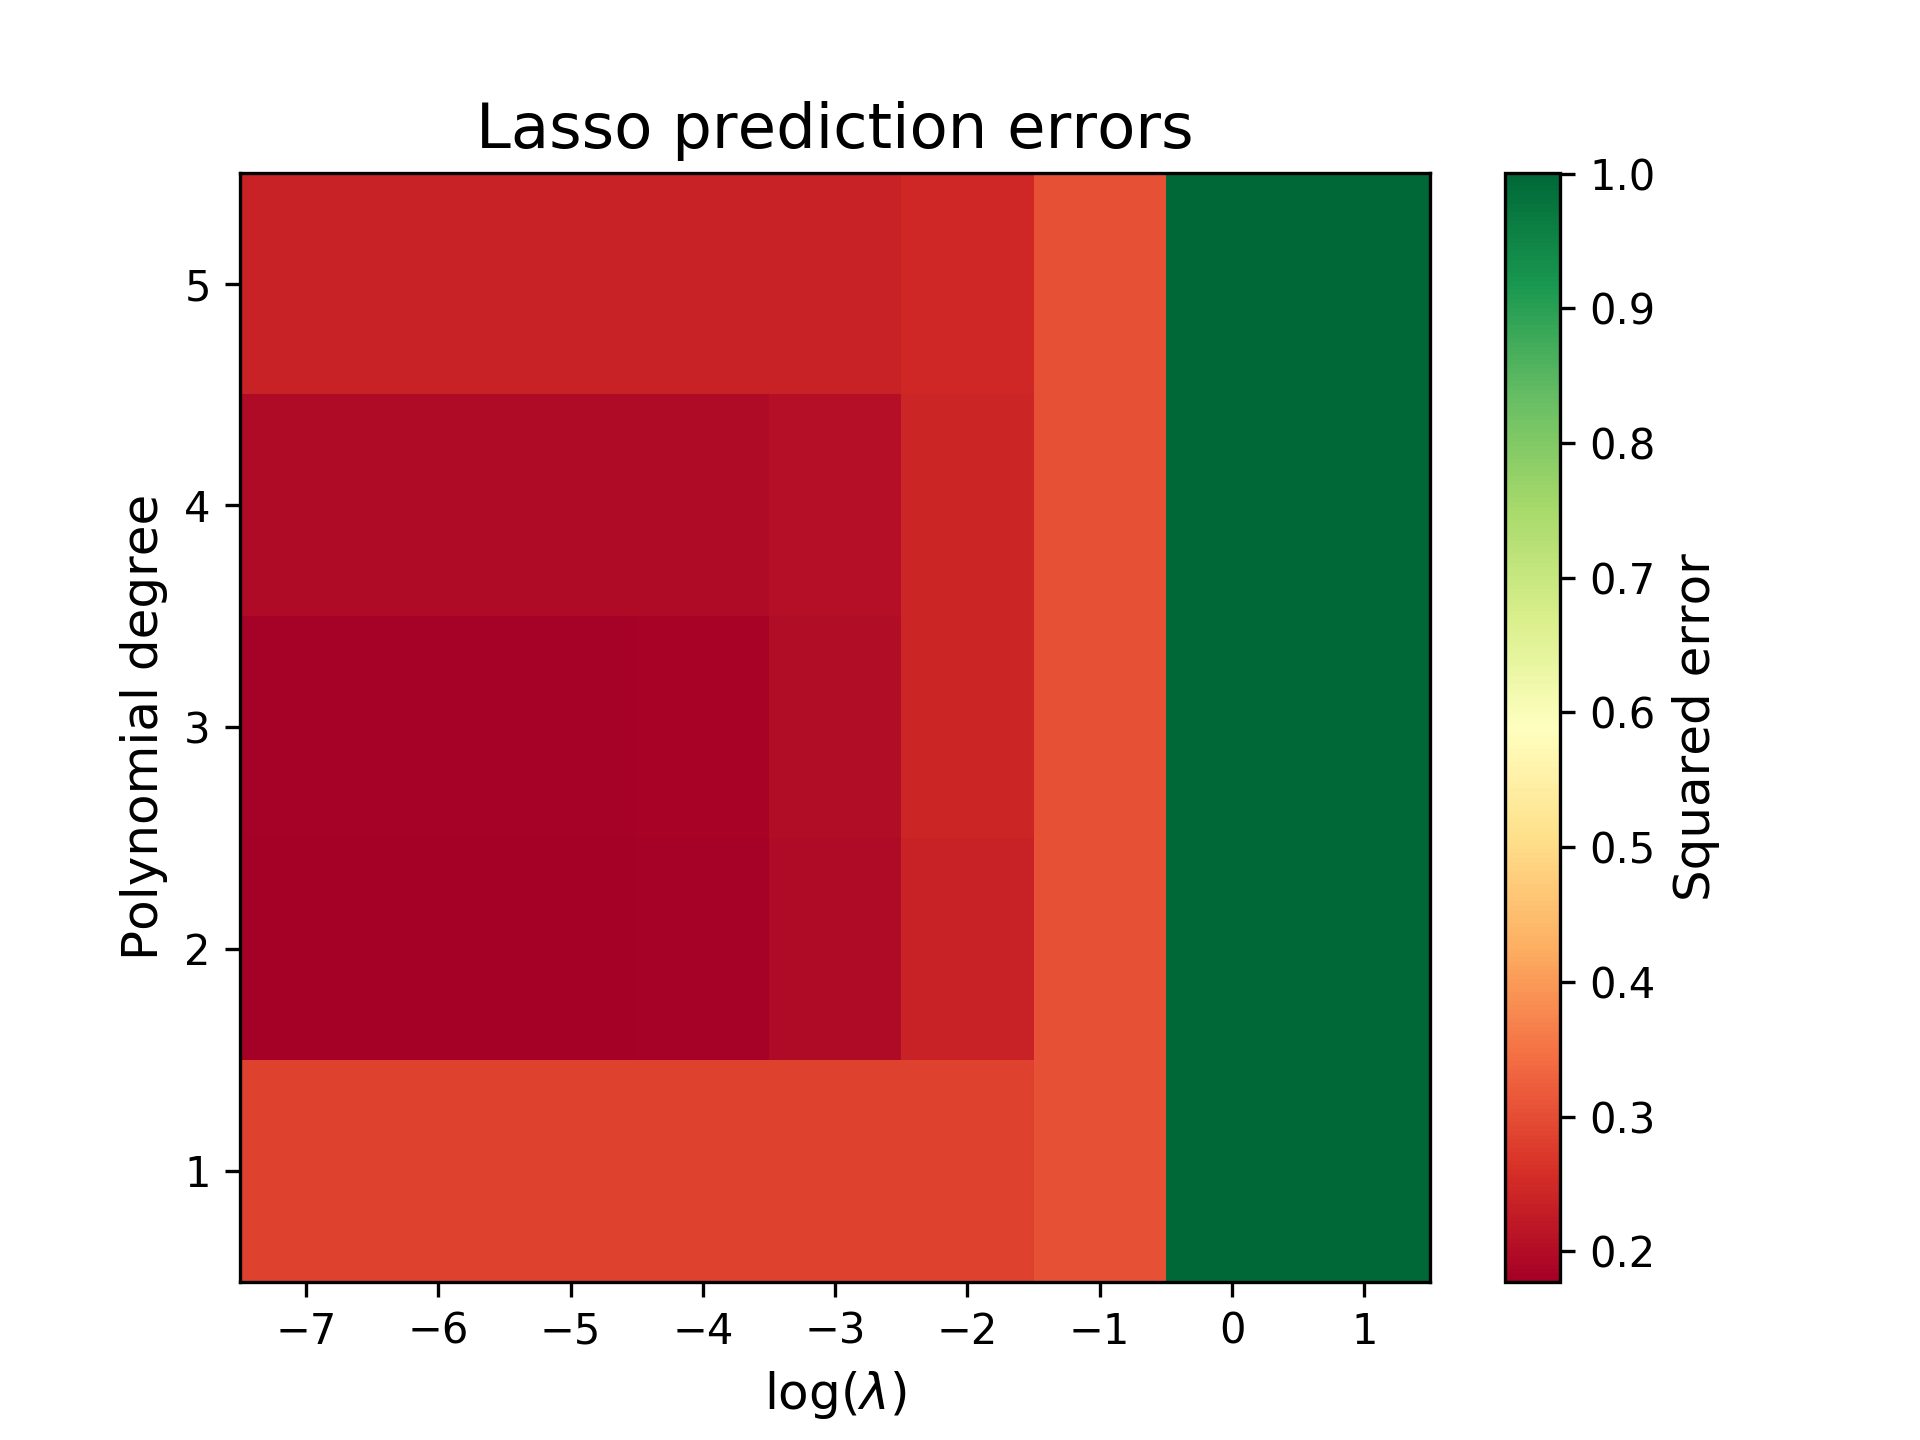
\includegraphics[width=0.45\textwidth]{../Figures/lasso_grid_search.png}
	\caption{The test MSE for each combination of penalties $\lambda$ and polynomial degrees for lasso regression of terrain data.}
	\label{fig23}
\end{figure}

\begin{figure}
	\centering
	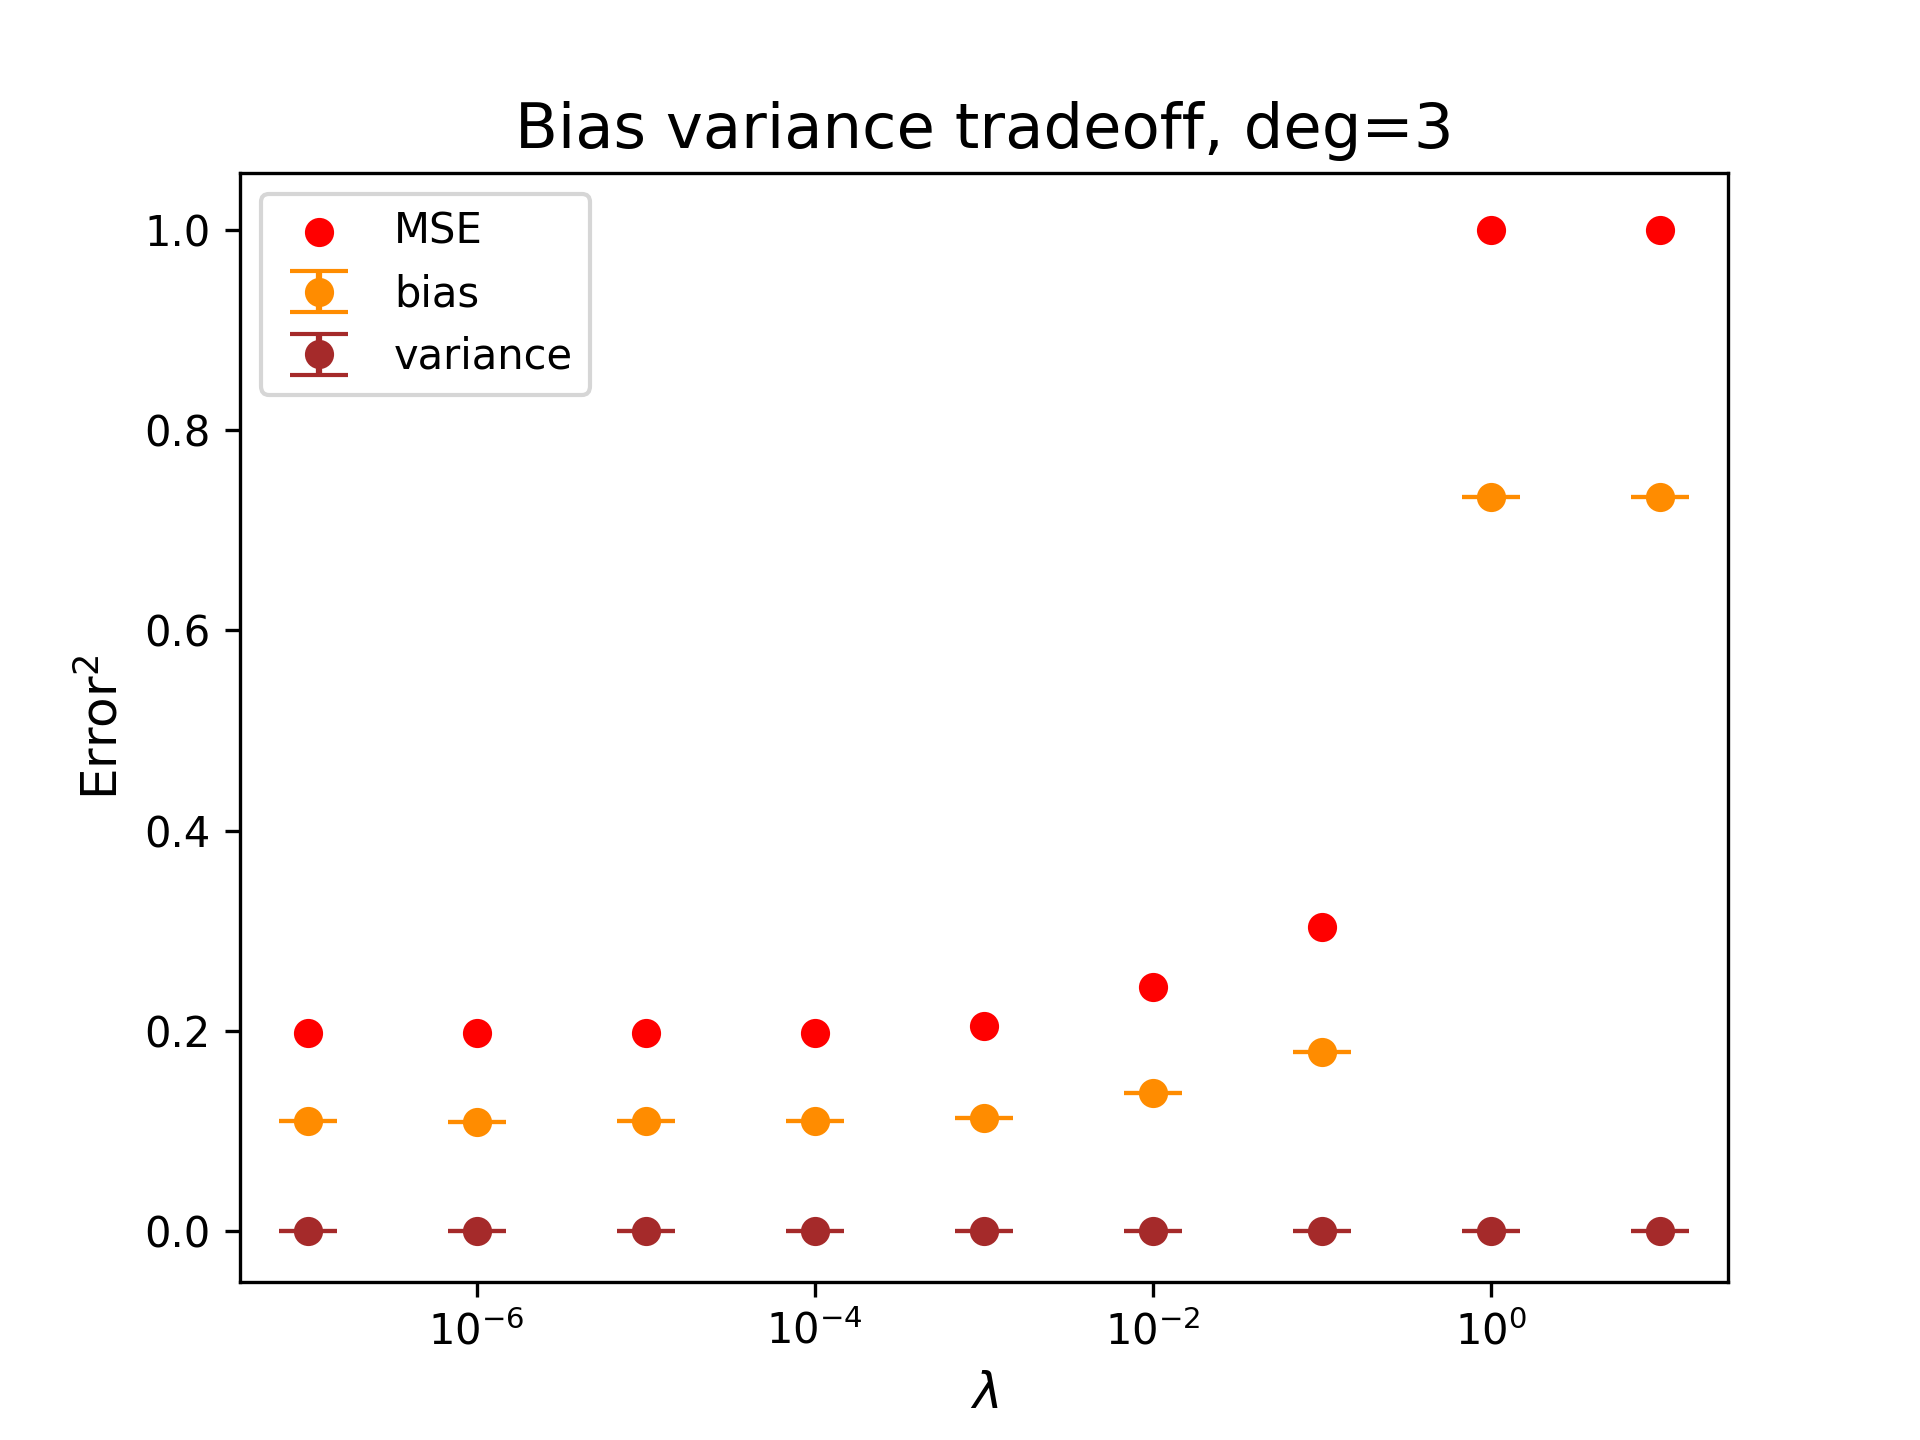
\includegraphics[width=0.45\textwidth]{../Figures/b-v_tradeoff_terrain_lasso_deg3.png}
	\caption{Bias variance tradeoff for a 3rd degree lasso approximation on terrain data.}
	\label{fig24}
\end{figure}

\clearpage

\begin{figure}
	\centering
	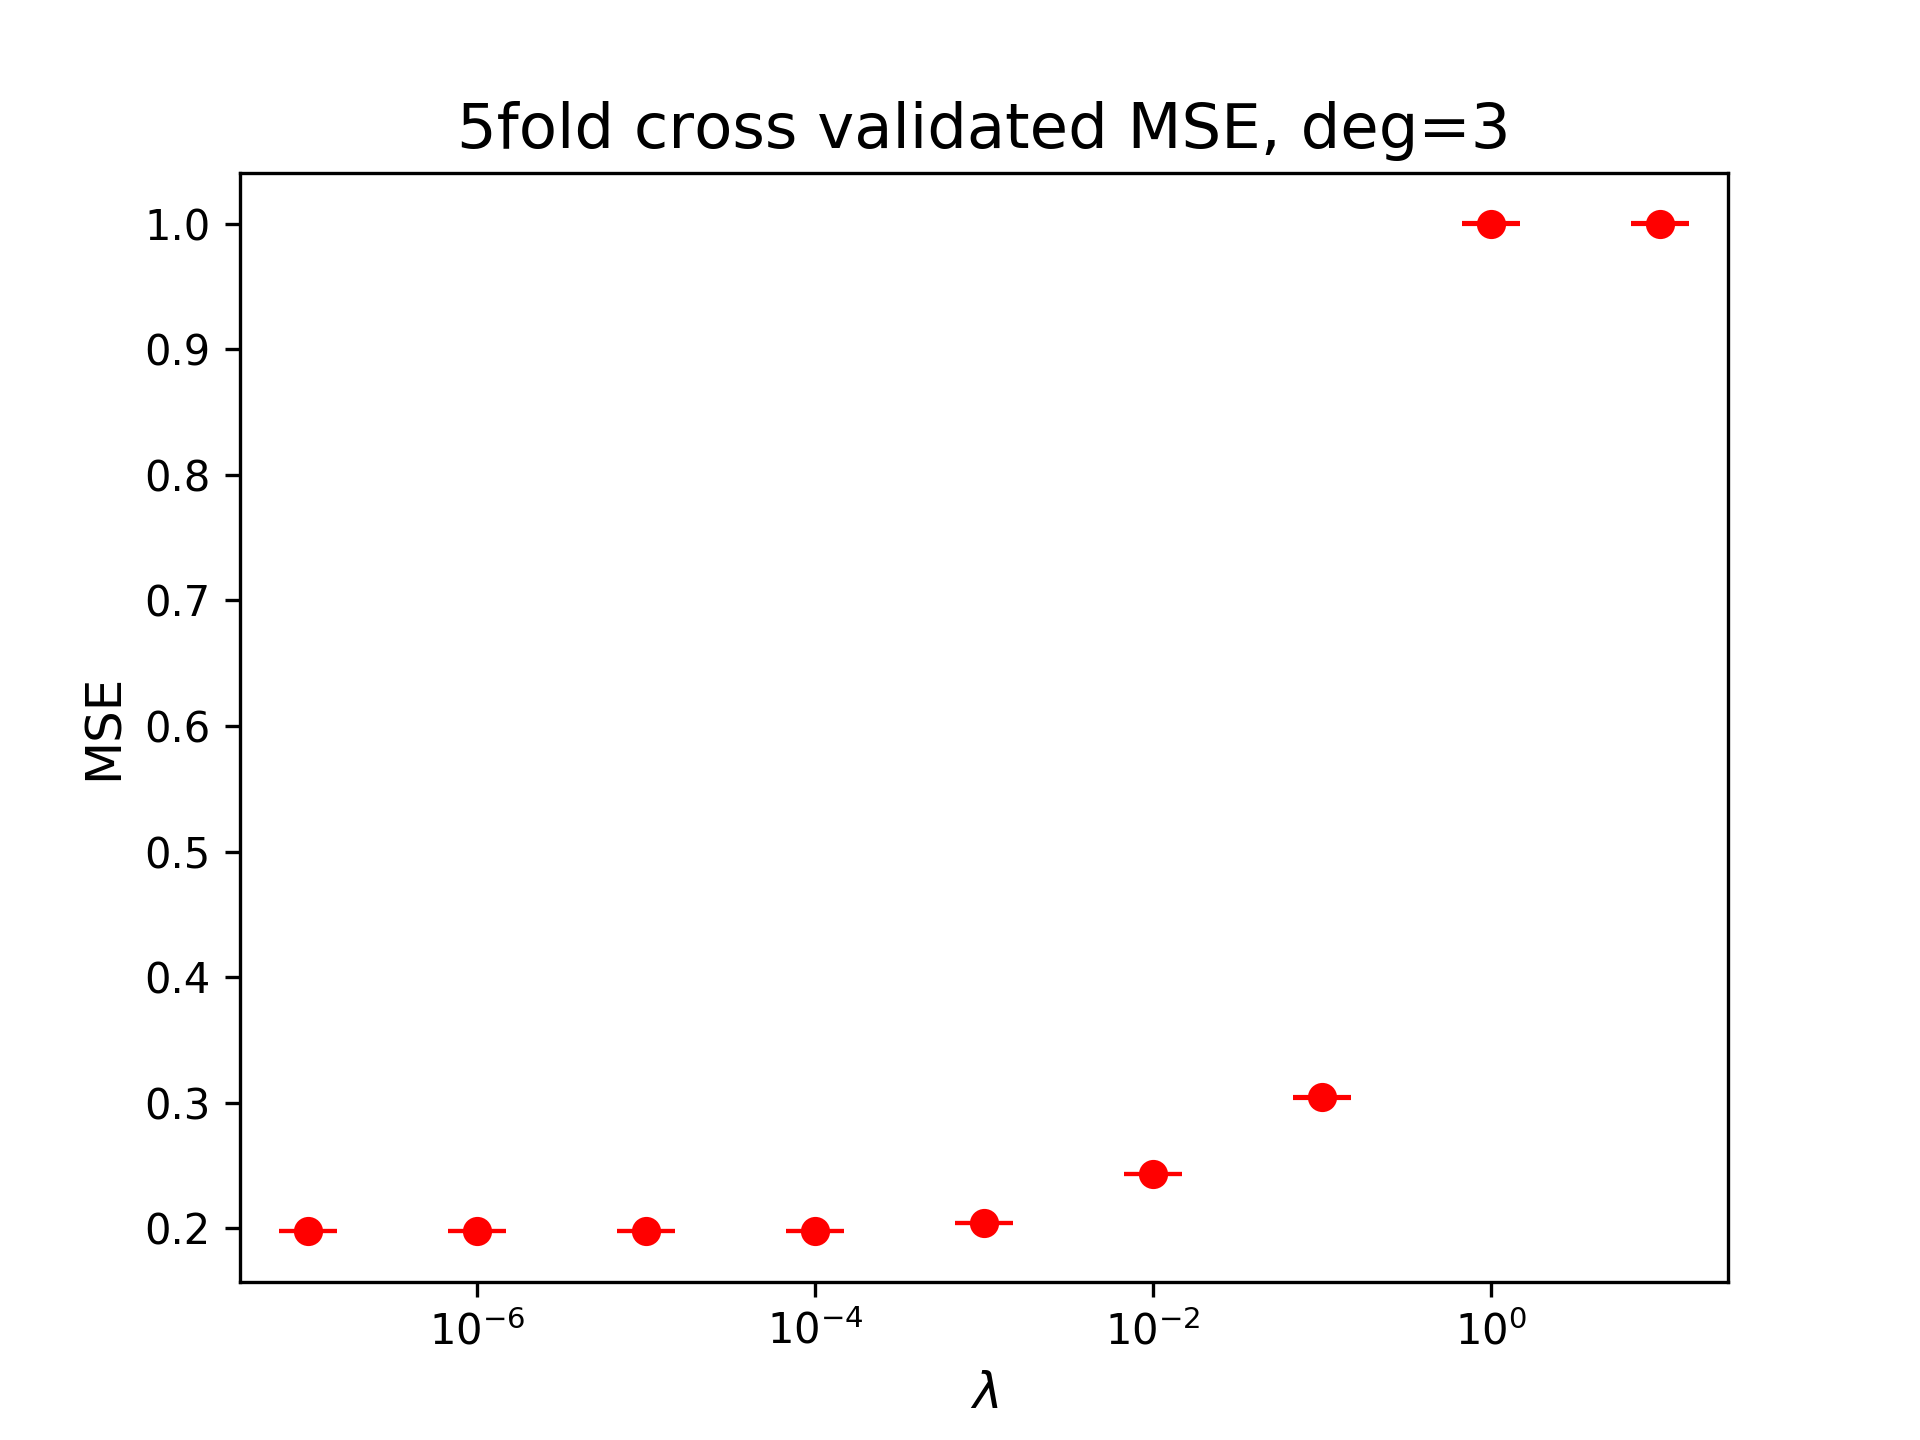
\includegraphics[width=0.45\textwidth]{../Figures/kfold_mse_terrain_lasso_deg3.png}
	\caption{5fold cross validation of penalties $\lambda$ for a 3rd degree lasso approximation on terrain data.}
	\label{fig25}
\end{figure}

\begin{figure}
	\centering
	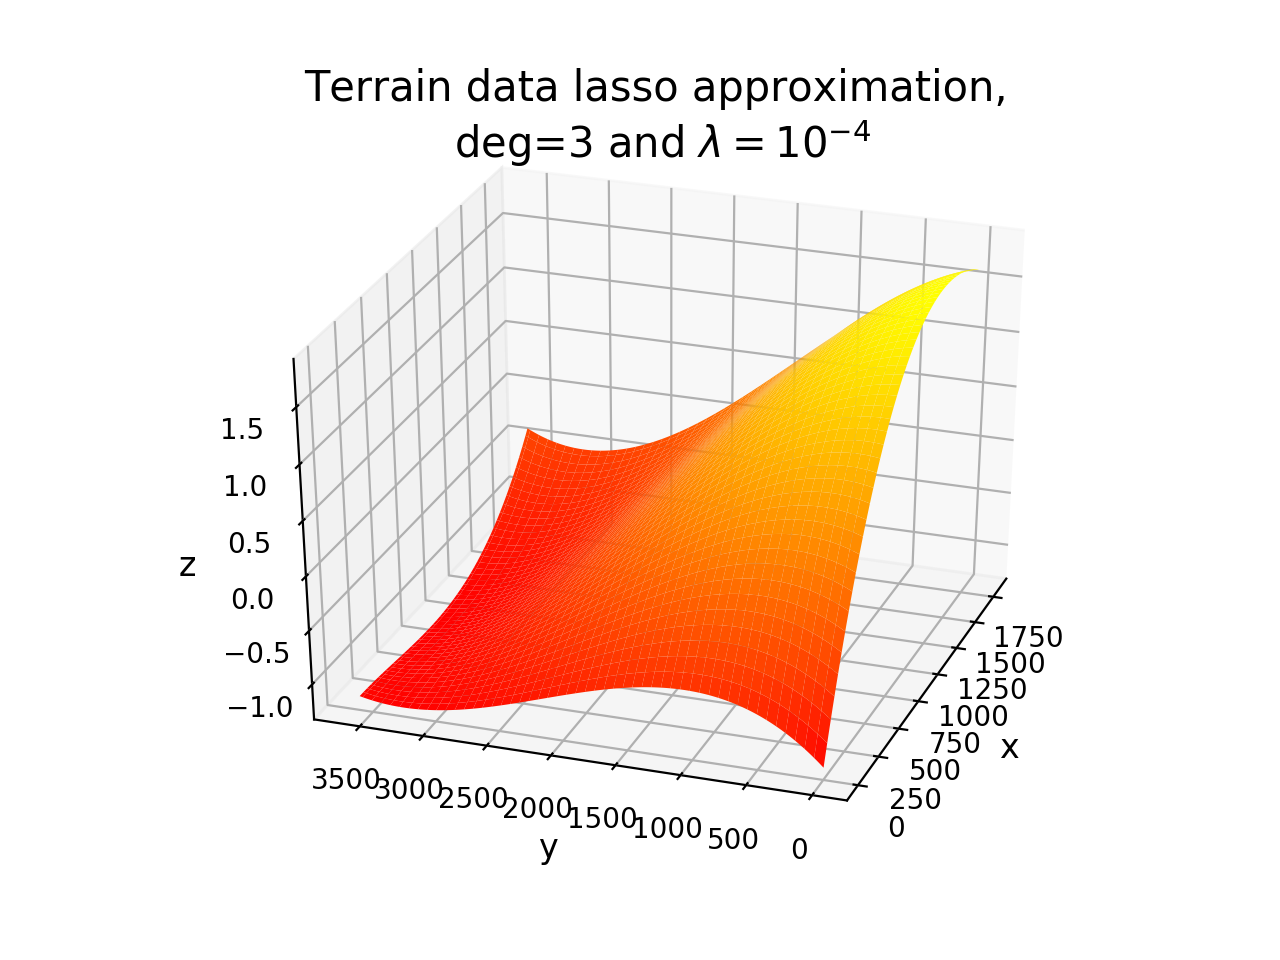
\includegraphics[width=0.45\textwidth]{../Figures/terrain_lasso_deg3_adjusted.png}
	\caption{3rd degree lasso approximation of terrain data with penalty $\lambda=10^{-4}$.}
	\label{fig26}
\end{figure}

\begin{figure}
	\centering
	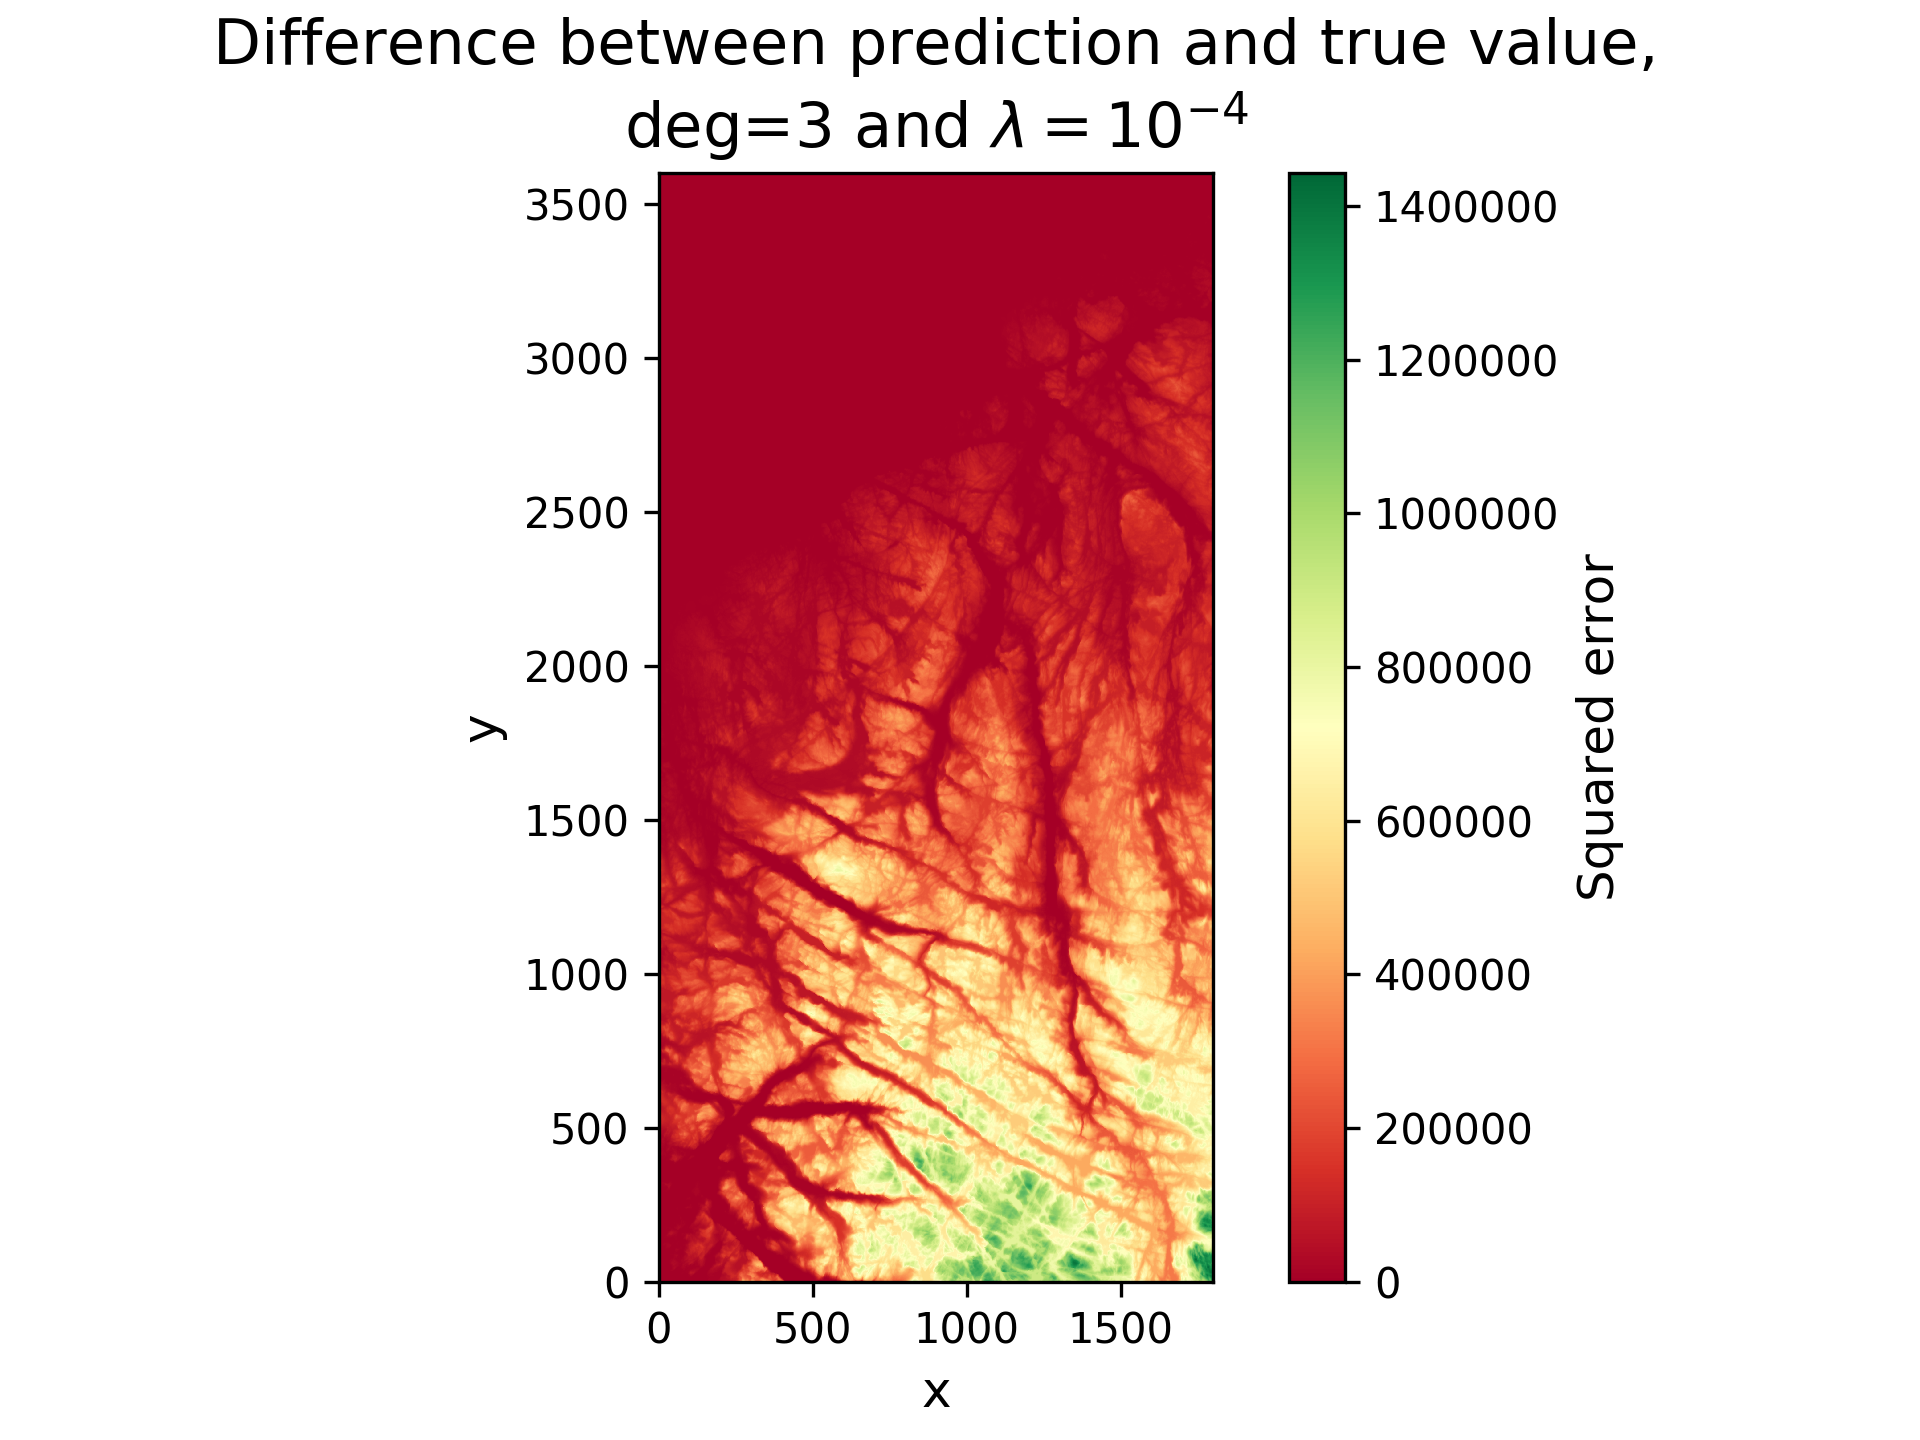
\includegraphics[width=0.45\textwidth]{../Figures/terrain_lasso_error_deg3.png}
	\caption{Errors of the 3rd degree lasso approximation of terrain data with penalty $\lambda=10^{-4}$.}
	\label{fig27}
\end{figure}

\clearpage
\section{Discussion}
For the Franke function, we noticed that a larger generated data set gave a better approximation. This makes sense, since the training set size increases when the total number of points increases. In addition, the higher polynomial degrees require more points for a fit to be possible, due to the high number of coefficients necessary. \\[2mm]
For the Franke function we got a bias variance tradeoff that showed no clear trends. This was the case for all three methods used. We would expect the variance to increase with the increase of polynomial degree (overfitting), but no such trends are visible. In addition, we would expect the bias to increase with the decrease of polynomial degree (underfitting). This trend is also absent. However, the 5fold cross validation gave results which were easy to interpret: a clear minimum error could be found. The optimal values for polynomial degree and penalty were therefore chosen based on the cross validation and not the bias variance plots. \\[2mm]
We found that the ridge and lasso methods were not significantly better than the OLS method for predicting the Franke data. It is possible that a better combination of penalty and polynomial degree could provide a better result. However, we found the computational cost of finding a better $\lambda$ to be very large compared to the observed benefits. A possible solution could be to investigate whether a different family of functions can provide better results than the polynomial family. \\[2mm]
The bias variance tradeoff was easier to interpret for the terrain data. Here we saw a clear variation. The 5fold cross validation results agreed with the bias variance tradeoff results. This is most likely due to the large size of the data set. \\[2mm]
The approximation error plots of the terrain data looked very different from the corresponding Franke plots. The vein-like patterns observed in the terrain error is a result of the highly irregular terrain surface. The Franke function is smooth, so the corresponding Franke error does not display this feature. All in all, the Franke function provided a good substitute for a terrain data set.

\section{Conclusion}
The aim of this project was to study parametrisation of surface data using linear regression methods with two dimensional polynomials. We used ordinary least squares, ridge and lasso regression and investigated polynomial degrees up to maximum 15. We found that while ridge and lasso provide an additional penalty parameter for adjusting the regression coefficients, the additional benefits were too small to make up for the added computational cost. \\[2mm]
Bootstrap was used to estimate the bias variance tradeoff in our models, but these results proved challenging to interpret. 5fold cross validation was used to estimate the true MSE. These results were much more interpretable and provided a clear picture of what parameters gave the best approximation. \\[2mm]
In general, we found that to parametrise surfaces using polynomials provided reasonable results. However, the polynomial approach was not able to capture irregular details typically found in real terrain data. 

\bibliographystyle{unsrtnat}
\bibliography{references.bib}






\end{document}